%%%%%%%%%%%%%%%%%%%%%%%%%%%%%%%%%%%%%%%%%
% University of Amsterdam master thesis title page 
% LaTeX Template
%
% Version 1.2 (14/02/14) (fixed cursive mode under titlepage)
%
% This template was made for the UvA by Ludo Nieuwenhuizen
% 
% 
% Instructions for using this template:
%
% I've done my best to make this template self-explanatory. The only thing (apart from
% finishing your thesis) is that wherever you see the percentage sign after some LaTeX
% commands, you have to insert some text (except for this
% introductory part, of course)l this is also explicitly stated.
%
% This title page can be compiled as is. This is not useful for 
% including it in another document. To do this, you have two options: 
%
% 1) Copy/paste everything between \begin{document} and \end{document} 
% starting at \begin{titlepage} and paste this into another LaTeX file where you 
% want your title page.
% OR
% 2) Remove everything outside the \begin{titlepage} and \end{titlepage} and 
% move this file to the same directory as the LaTeX file you wish to add it to. 
% Then add \input{./titlepage_master_thesis.tex} to your LaTeX file where you want your
% title page.
%
% The layout is quite vulnerable for changes. If you for instance remove the logo at the
% bottom, the last line 'Department Research institute...' will get higher up the page. In this 
% case it is safer to insert a blank image or fix it in a different way.
%
% Any questions can be sent to me (L.G.Nieuwenhuizen@gmail.com)
%%%%%%%%%%%%%%%%%%%%%%%%%%%%%%%%%%%%%%%%%

\documentclass[11pt,twoside,a4paper,fleqn]{report}

\usepackage{graphicx}
\usepackage{graphics}
\usepackage[english]{babel}
\usepackage[hcentering,bindingoffset=8mm]{geometry}
\usepackage[utf8]{inputenc}
% \usepackage[en-US]{datetime2}
\usepackage{amssymb}
\usepackage{amsmath}
\usepackage{natbib}
\usepackage[colorlinks=true, allcolors=blue]{hyperref}
\usepackage{caption}
\usepackage{tocloft}
\usepackage{amsfonts}
\usepackage[section]{placeins}
\usepackage{fancyhdr}
% \usepackage{siunitx}
\usepackage{subcaption}
\usepackage{listings}
\usepackage{acro} 
%\usepackage{abbriv}
\usepackage{longtable}
\usepackage{array}
\usepackage{tablefootnote}
\usepackage{epigraph}
\usepackage{comment}
\usepackage{float}
\usepackage{adjustbox}
\usepackage[capitalise]{cleveref}
\usepackage{titlesec}
\usepackage{multicol}
\usepackage{multirow}

\setcounter{secnumdepth}{4}




\graphicspath{{folder/}{../figures/}}

\pagestyle{fancy}
\fancyhead[RO]{\fancyplain{}{\nouppercase{\leftmark}}}
\renewcommand\sectionmark[1]{\markboth{\MakeUppercase{#1}}{}}
\fancyhead[LO]{}
\fancyhead[LE]{\fancyplain{}{\nouppercase{\leftmark}}}
\renewcommand\sectionmark[1]{\markboth{\MakeUppercase{#1}}{}}
\fancyhead[RE]{}
\lfoot{}
\cfoot{\fancyplain{}{\thepage}}
\rfoot{}

% \sisetup{separate-uncertainty, multi-part-units = brackets}
% \DeclareSIUnit\parsec{pc}
% \DeclareSIUnit\photons{ph}
% \def\kms{km~s$^{-1}$}

\newcolumntype{L}[1]{>{\raggedright\let\newline\\\arraybackslash\hspace{0pt}}m{#1}}

%\setlength{\headheight}{15pt}

%\parskip = \baselineskip

\captionsetup[table]{name=Table,labelfont={sc,footnotesize},textfont=footnotesize,labelsep={1in}}
\captionsetup[figure]{name=Fig.,labelfont={sc,small},textfont=footnotesize,labelsep=endash}
\numberwithin{equation}{chapter}
\numberwithin{figure}{chapter}

\newcommand{\vdag}{(v)^\dagger}
\newcommand\aastex{AAS\TeX}
\newcommand\latex{La\TeX}

\setlength{\parindent}{0 cm}
\pagenumbering{gobble}

\acsetup{list-style=longtable}
\DeclareAcronym{rlof}{
  short = RLOF ,
  long = Roche-lobe overflow
}

\DeclareAcronym{ms}{
  short = MS ,
  long = main-sequence
}

\DeclareAcronym{rgb}{
  short = RGB ,
  long = red giant branch
}

\DeclareAcronym{agb}{
  short = ABG ,
  long = asymptotic giant branch
}

\DeclareAcronym{he}{
  short = HE ,
  long = hydrostatic equilibrium
}

\DeclareAcronym{te}{
  short = TE ,
  long = thermal equilibrium
}

\DeclareAcronym{hrd}{
  short = HRD ,
  long = Hertzsprung-Russel diagram
}

\DeclareAcronym{zams}{
  short = ZAMS ,
  long = zero age main-sequence
}

\DeclareAcronym{tams}{
  short = TAMS ,
  long = terminal age main-sequence
}

\DeclareAcronym{rsg}{
  short = RSG ,
  long = red super-giants
}

\DeclareAcronym{rl}{
  short = R$_L$ ,
  long = Roche lobe radius
}

\DeclareAcronym{sph}{
  short = SPH ,
  long = Smooth Particle Hydrodynamics
}

\DeclareAcronym{eos}{
  short = EOS ,
  long = equation of state
}

\DeclareAcronym{wd}{
  short = WD ,
  long = white dwarf
}


%Roche lobe radius, $R_{L}$
 

\begin{document}
\begin{titlepage}

\newcommand{\HRule}{\rule{\linewidth}{0.8mm}}
\center
 \vspace*{0.5cm}  % Play around with this as you want
% ------
% Heading20
% ------
\raisebox{0.05cm}[0pt][0pt]{
\includegraphics[width=2.0cm]{Thesis/logos/UvA_logo.png}}
\raisebox{0.7cm}[0pt][0pt]{\textsc{\Huge University of Amsterdam}}
\raisebox{-1.85cm}[0pt][0pt]{
\includegraphics[width=7.0cm]{Thesis/logos/VUlogo.png}}\\[2.0 cm]

\Large{\textbf{MSc Physics and Astronomy}}\\% Study discipline
\Large{Track: Astronomy \& Astrophysics}\\[0.7cm] % Master track name
\textsc{\Large \textbf{Master Thesis}}\\[0.2cm]

% -----
% Title
% -----

\HRule \\[0.3cm]

{ \huge \bfseries Mass Transfer in Hierarchical Triple Systems:
}\\[0.8cm] % title of thesis
{\Large \bfseries The Case of Roche-Lobe filling Outer Star} % subtitle of thesis

\HRule \\[0.7cm]
 
% -----
% Details
% -----

{\Large \emph by}\\[0.6cm]
{\Large \bfseries Adam Parkosidis\\ % student name
13950142}\\[0.4cm] %student ID
%\DTMlangsetup{showdayofmonth=false}
{\large  \emph{\today}}\\ % month + year in which the thesis was concluded
%\DTMlangsetup{showdayofmonth=true}
{\large  \emph{60 ECTS}}\\ % 'this many' ects that are rewarded for the thesis
{\large  \emph{01/11/2022 - 30/07/2023}}\\[1.8cm] % period in which the research was carried out

% -----
% Supervisor, etc.
% -----

\begin{minipage}{0.4\textwidth}
\begin{flushleft} \large
{\large \emph{Supervisors:}}\\

\large{Dr Silvia Toonen}\\ % Supervisor's Name
\large{Dr Philipp Moesta}
\end{flushleft}
\end{minipage}
~
\begin{minipage}{0.4\textwidth}
\begin{flushright} \large
\emph{Examiners} \\
\large{Dr. Silvia Toonen} \\
\large{Dr. Oliver Porth} % Examiner's Name
\end{flushright}
\end{minipage}\\


% -----
% Logo and Department
% -----

\raisebox{-138pt}[0pt][0pt]{\includegraphics[width=5.5cm]{Thesis/logos/api_logo.pdf}}\\ % Call your institute logo "institute.jpg", or be creative.

% \raisebox{-138pt}[0pt][0pt]{\large{Anton Pannekoek Institute for Astronomy}} %name of the department or institute or company


% -----
% That was easy, right?
% -----

\vfill 

\end{titlepage}

\newpage
\chapter*{Abstract}

Mass transfer in hierarchical triple systems, and more specifically, \ac{rlof} by the outer star, is expected to be considerably different from mass transfer in an ordinary binary system. The mass cannot be simply accreted by the inner objects, but may instead form a circumbinary disk or be expelled via a slingshot effect due to the inner binary rotation. Stellar evolution, gravitational dynamics, and hydrodynamics all play important roles in the process. In the first part, we create 3D hydrodynamical models of post main-sequence stars based on detailed 1D stellar evolution models. In the second part, we use AMUSE to couple hydrodynamics with high accuracy gravitational integrators and solve these physical processes in a self-consistent  manner. Hence, we simulate the phase of mass transfer in a hierarchical triple system in which the tertiary star will overfill its Roche lobe before any of the inner stars leave the main sequence. We encounter a fairly non-conservative mass transfer, and while we quantify its impact on the inner and outer orbits, predicting the end of the mass transfer phase and the appearance of the resulting system is difficult. However, we provide some preliminary estimations of the system's accretion efficiency and the amount of angular momentum lost. Finally,
we speculate that the formation of a circumbinary disk around the inner binary probably leads to significantly more conservative mass transfer. 





\mbox{}


\newpage
\pagenumbering{roman}
\setcounter{page}{1}
{
  \hypersetup{linkcolor=black}
\tableofcontents

%\begin{comment}
\newpage
\thispagestyle{empty}
\mbox{}
\newpage

\listoffigures

\newpage
\thispagestyle{empty}
\mbox{}
\newpage

\listoftables

\newpage
\thispagestyle{empty}
\mbox{}
\newpage

\mbox{}
\thispagestyle{empty}
\printacronyms[include-classes=abbrev,name=List of Abbreviations]


}






%\DeclareAcronym{he}{
%  short=HE,
%  long=Hydrostatic Equilibrium,
%}

%\end{comment}

\newpage
\thispagestyle{empty}
\mbox{}
\newpage

\pagenumbering{arabic}
\setcounter{page}{1}


\parskip = 2mm

\chapter{Introduction} \label{introduction}

\epigraph{The stars are not lonely, in their shining solitude. They have each other, and they have us.}{Isaac Asimov}


Observations proved that field stars are not always single; many develop in pairs, and many of these binaries are members of triples or higher-order systems. Additionally, the fraction of systems with companions grows with mass (see \cref{fig:stellar_companions}), as a result massive stars are seldomly formed in isolation. In contrast, many intermediate- and high-mass stars are created in binary or higher order multiple systems with $\sim 50\%$ of spectral type B stars be in triples \citep{sana2014southern,moe2017mind}, a percentage which reduces to $\sim 10\%$ for low-mass stars \citep{raghavan2010survey,toonen2014popcorn,moe2017mind}. In these cases, apart from the intrinsic stellar properties, the evolution depends sensitively on the interaction between the system's stellar components. Consequently, triple systems are not as uncommon as we may mistakenly believe, particularly in the concept of intermediate- and high-mass stars.

Although the fundamentals of single and binary evolution have long been acknowledged \citep{postnov2014evolution,toonen2014popcorn}, the long-term evolution of stellar triples remains unknown. In the simple case, stable triple systems, which are hierarchical, namely, consist of an inner and an outer binary orbit, i.e., the tertiary (third object). The secular evolution of such systems is the modification of orbital elements over timescales substantially larger than the system's dynamical timescale. Hence, the presence of the outer star has no influence on the history of the inner binary and the evolution of the inner binary and the tertiary can be discussed independently. In other cases, a third star in orbit around a binary system can drastically influence the system's development
via dynamical interactions, which influence the orbital elements of the inner and outer orbit through changes in energy and angular momentum. Consequently, hierarchical triple star systems can become unstable via triple stellar evolution processes which are unique to systems with multiplicities of higher orders than binaries.
\begin{figure}[H]
    \centering
    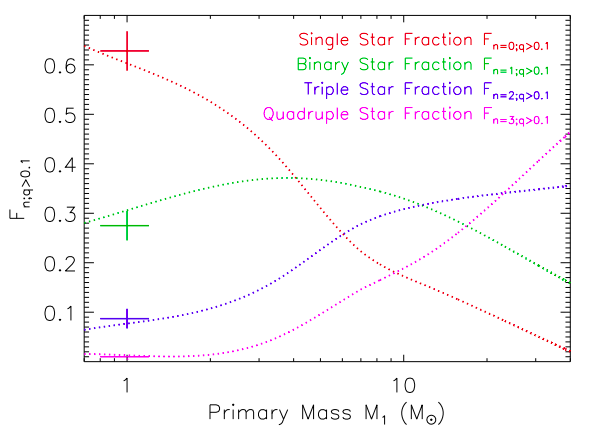
\includegraphics[width=\textwidth]{Thesis/figures/fig_moe_2017.png}
    \caption{Multiplicity fractions as a function of primary mass (dotted lines), including the single-star $F_{n=0;q> 0.1}$ (red), binary-star $F_{n=1;q> 0.1}$  (green), triple-star $F_{n=2;q> 0.1}$  (blue), and quadruple-star fraction $F_{n=3;q> 0.1}$  (magenta). Given a primary mass $M_1$, the model assumes that the multiplicity fractions follow a Poisson distribution across the interval $n = [0, 3]$ in a manner that reproduces the measured multiplicity frequency $F_{mult;q >0.1} = \Sigma_{n=1}^3 \; n F_{n;q> 0.1}$. For solar-type stars, this model matches the measured values (solid) within their uncertainties. Regardless of the uncertainties in the multiplicity fractions, $\leq 10\%$ of O-type stars are single while $\geq 55\%$ are born in triples and/or quadruples. Figure taken by \cite{moe2017mind}.}
    \label{fig:stellar_companions}
\end{figure}
The rich dynamical behavior of three-body systems can produce Lidov-Kozai cycles, in which the eccentricity of the inner orbit and the inclination between the inner and outer orbits vary periodically \citep{michaely2014secular,toonen2016evolution,mangipudi2022extreme}. As a result, tidal effects (tidal friction), gravitational-wave emission, and stellar interactions such as mass transfer, angular momentum exchange and collisions may be enhanced. In this way, evolution in triples can give rise to stellar mergers \citep{antonini2017binary,silsbee2017lidov,vigna2021massive}, namely some of most energetic events in the universe, ranging from gravitational wave sources to electromagnetic transients, e.g. luminous red novae, and also provide promising evolutionary pathways for exotic objects \citep{sana2012binary, toonen2016evolution}, e.g. blue stragglers \citep{winn2009spin}. In the past, most of our efforts in understanding the progenitors of the events were focused on modeling binary evolution disregarding the interaction of the binary with a third star. Therefore, a detailed examination of triple evolution is as necessary as it is challenging because it demands a self consistent treatment of three-body dynamics and stellar evolution.

\section{Goal \& Scientific Questions}

In this thesis, I investigate a hierarchical triple system in which the tertiary star will eventually overflow its Roche lobe before any of the inner stars leave the main sequence. The goal is to thoroughly examine the mass transfer phase by creating detailed hydrodynamical simulations, evaluate the significance of various parameters in the process, and speculate on the resulting evolution.

There are two main scientific questions that I try to tackle:

\begin{itemize}
    \item How does mass transfer affect the evolution of the inner and outer orbital parameters?
    \item How does the binary's accretion affect the evolution of the inner and outer orbital parameters?
\end{itemize}




\section{Target system: $\xi$ Tau}

$\xi$ Tau is a hierarchical triple system with orbital parameters that are relatively well constrained. The evolution of the system was initially examined by \cite{de2014evolution}, where they  concluded that it is likely to develop \ac{rlof} near the end of the first \ac{agb}, roughly halfway to type B mass transfer \citep{kippenhahn1967entwicklung}.

To further restrict the system's orbital characteristics, \cite{nemravova2016xitauri} combined a large series of spectroscopic photometric (including space-borne) observations with long-baseline optical and infrared spectro-interferometric observations. They show, using perturbation theory, that prominent secular and periodic dynamical effects may be explained by a quadrupole interaction. Despite this, the orbital parameters of the third orbit remain unclear due to the low relative brightness of the most distant star.

I use the orbital parameters given in \cite{2010yCat..73890925T} in my study. The rationale for this is so that I can compare my results to \cite{de2014evolution}. The orbital parameters of $\xi$ Tau are given in \cref{tab:system_orbit_param}.
\begin{table}[H]
    \centering
    \begin{tabular}{|c c c c c c c c|}
       Name & M$_1$ (M$_{\odot}$) & M$_2$ (M$_{\odot}$) &
       M$_3$ (M$_{\odot}$) & $P_{in}$ (day) &
       $P_{out}$ (day) & $\epsilon_{in}$ &
       $\epsilon_{out}$ \\
       \hline
       HD 21364 & 3.2 & 3.1 & 5.5 & 7.15 & 145.5 & 0.0 & 0.15
    \end{tabular}
    \caption{Orbital parameters of $\xi$ Tau system. Masses $M_1$ and $M_2$ correspond to the inner binary components, while $M_3$ is the mass of the tertiary. The orbital period and eccentricity of the inner and outer orbit are given with the subscripts $in$ and $out$, respectively.}
    \label{tab:system_orbit_param}
\end{table}
In their analysis, \cite{nemravova2016xitauri} constrain  the mutual inclination between the two orbits, i.e. the inclination of the outer orbit relative to the inner orbit, concluding that they are nearly coplanar. Mutual inclination, $i_{mut}$, is expected to have the strongest effects on the mass transfer, thus it is a free parameter to be explored.


\section{Thesis outline}

The remainder of this thesis is organized into four chapters. Each chapter starts with a short introduction, while the chapters are structured as follows: 

In the second chapter, I present an overview of single star evolution with a focus on intermediate-mass stars, because this is the mass regime of interest for my target system. I also constrain myself in evolution aspects that are relevant for my hydrodynamical models. Furthermore, I discuss concepts of binary evolution and I argue how to extend these to the triple evolution case. In the remainder of the second chapter, I provide information about the scientific codes, utilized in my simulations. In chapter three, I display the methods used to build my hydrodynamical models, their underlying assumptions and their physical justification. Furthermore, I present the initial setup of my simulations. In chapter four, I demonstrate my results, while a detailed discussion follows in chapter five.








\chapter{Background}\label{background}

\epigraph{The stars are not distant objects to be admired from afar. They are our partners in exploration and discovery, and we must learn to live and work with them if we are to achieve our goals.}{Arthur C. Clarke}

The evolution of a star in isolation, namely single star evolution, is predominantly determined by the stellar mass. Stars with $M \leq 2$ M$_{\odot}$, $2 < M \leq 8$ M$_{\odot}$ and $M > 8$ M$_{\odot}$ are classified as low-, intermediate-, and high-mass, respectively. In their attempt to achieve hydrostatic and thermal equilibrium, stars generate temperatures and pressures that allow for nuclear burning. The cycles of nuclear burning and fuel exhaustion regulate the evolution of a star and set the various phases during the stellar lifetime. These burning cycles can be viewed as long-lived, but transient disruptions to a star's (or at least its core's) inexorable shrinkage under the effect of gravity. The virial theorem dictates, that this contraction is caused by the fact that stars are hot and lose energy through radiation. 







\begin{comment}
 Despite the inherent rarity predicted by the initial mass function (IMF, see e.g. \cite{chabrier2005initial, dib2018emergence}), massive stars play a key role in the evolution of the Universe. They are the main source of UV radiation and heavy elements. They serve as a significant source of mixing and turbulence in the interstellar medium (ISM) of galaxies through a combination of winds, outflows, expanding HII regions, and supernova explosions. Galactic dynamos are powered by turbulence in conjunction with differential rotation. Cosmic rays are accelerated by the interaction of galactic magnetic fields and supernova shock fronts. The ISM is primarily heated by cosmic rays, UV radiation, and the dissipation of turbulence, whereas it is finally cooled by heavy metals present in dust, molecules, and in atomic/ionic form. Therefore, massive stars have a significant impact on galaxies' physical, chemical, and morphological structure \citep{kennicutt2005role}. However, the physical mechanisms behind the birth, development, and demise of massive stars remain elusive in comparison with low-mass stars \citep{zinnecker2007toward}. 
\end{comment}

\section{Timescales of stellar evolution}\label{sec:timescales}

The fundamental timescales of stellar evolution are the dynamical, thermal and nuclear timescales. The dynamical timescale is the characteristic time required for a star to collapse under its own gravitational force in the absence of internal pressure:
\begin{equation}\label{eq:dynamical_timsecale}
    t_{dyn} = \sqrt{\frac{R^3}{GM}} \sim 0.02 \left( \frac{R}{R_{\odot}} \right)^{3/2} \left( \frac{M}{M_{\odot}}\right)^{1/2} \; \text{days},
\end{equation}
where $R$ and $M$ are the star's radius and mass. It is a period on which a star might expand or contract if its hydrostatic equilibrium were disrupted, e.g. in case of sudden mass-loss.

Thermal (or Kelvin-Helmholtz) timescale indicates how quickly changes in a star's thermal structure may occur. It is therefore also the period on which a star responds when its thermal equilibrium is disturbed:
\begin{equation}\label{eq:thermal_timsecale}
    t_{th} = \frac{G M^2}{2RL} \sim 1.5 \times 10^7 \left( \frac{M}{M_{\odot}} \right)^{2} \frac{R_{\odot}}{R} \frac{L_{\odot}}{L} \; \text{yr},
\end{equation}
where L is the star's luminosity.

Finally, the nuclear timescale corresponds to the time required for the star to exhaust its nuclear fuel supply at its current luminosity: 
\begin{equation}\label{eq:nuclear_timsecale}
    t_{nuc} = \frac{\phi M_{nucl} c^2}{L} \sim 10^{10} \frac{M}{M_{\odot}} \frac{L_{\odot}}{L} \; \text{yr},
\end{equation}
where $\phi$ is the efficiency of nuclear energy production, $M_{nuc}$ is the amount of mass available as fuel, and $c$ is the light speed. For core hydrogen burning, $\phi = 0.007$ and $M_{nucl} \sim 0.1 M$ \citep{pols2011stellar}.

Typically $t_{nuc} >> t_{th} >> t_{dyn}$, while assuming a mass-luminosity relation of $L \propto M^{\alpha}$, with empirically $\alpha \sim 3-4$ \citep{eker2015main}, it follows that intermediate- and high-mass stars live shorter and evolve faster than low-mass stars.

%\subsection{Hertzsprung-Russell Diagram}\label{sub:HR_diagram}

\section{Evolution of intermediate-mass stars in isolation}\label{sec:single_star_evolution}

\begin{comment}

The late stages of their evolution, namely the Asymptotic Giant Branch (AGB) phase, is characterized by rich nucleosynthesis and strong mass loss, that eventually removes their envelopes, leaving behind a degenerate C-O core as the central star of a planetary nebula\citep{pols2011stellar}. Additionally, the lost mass provides material for future generations of stars, 
\end{comment}


The \ac{hrd} diagram is a useful tool for studying stellar evolution. It is a logarithmic representation of the surface luminosity (or absolute magnitude) of a star as a function of its effective temperature (or spectral type). Furthermore, it is divided into five different regions, namely the \ac{ms}, the \ac{rgb}, the horizontal-giant branch, the \ac{agb} and the region of degenerate stars. A star, depending on its mass, will pass through some of these regions during its lifetime as a result of the interplay between nuclear reactions and gravitational contraction. 

\begin{figure}[H]
    \centering
    \includegraphics[width=0.9\textwidth]{Thesis/graphs/HR_inter_stars.pdf}
    \caption{Hertzsprung-Russell diagram. Evolutionary tracks for three stars with masses 3, 5.5 and 8 M$_{\odot}$ at solar metallicity until the end of Helium burning. Specific moments in the evolution of the stars are noted by black circles and squares as explained in the text. I calculate the tracks using MESA \citep{paxton2010modules,paxton2013modules,paxton2015modules,paxton2019modules}. The dashed lines show lines of constant radii by means of the Stefan–Boltzmann law.}
    \label{fig:HR_inter_stars}
\end{figure}
Intermediate-mass stars have a complex evolutionary path that includes multiple phases of fusion and contraction. The \ac{hrd} diagram in \cref{fig:HR_inter_stars} shows three evolutionary tracks for intermediate-mass stars. From left to right, the black circles correspond to the \ac{zams} and \ac{tams}. At \ac{zams}, the star having started the hydrogen burning in its core, achieves \ac{te}, $L_{nuc}/L =1$, while \ac{tams} is defined as the core hydrogen exhaustion point. Additionally, the black squares represent the start and end of helium burning in the core, respectively.
\ac{tams} and the end of helium burning in the core are both defined as the point at which the hydrogen and helium core mass fractions are $< 0.01$, respectively. The change in the star's physical radius occurs on different timescales depending on the physical mechanism buried beneath these processes. On nuclear timescale, see \cref{eq:nuclear_timsecale}), stars evolve throughout the \ac{ms} and the helium-burning phase, while on thermal timescale (see  \cref{eq:thermal_timsecale}), stars expand during the H-shell burning phase.
\begin{figure}[H]
    \centering
    \includegraphics[width=0.9\textwidth]{Thesis/graphs/HR_evolution.pdf}
    \caption{Evolution of 5.5 M$_{\odot}$ at solar metallicity until a the end of the early \ac{agb} phase. The evolutionary phases are categorized in different colors as explained in the text. I calculate the tracks using MESA \citep{paxton2010modules,paxton2013modules,paxton2015modules,paxton2019modules}. The dashed lines show lines of constant radii by means of the Stefan–Boltzmann law.}
    \label{fig:HR_evolution}
\end{figure}
\cref{fig:HR_evolution} illustrates the evolution of a 5.5 M$_{\odot}$ star in isolation from the beginning of the \ac{ms} until the end of the early \ac{agb} phase. The evolutionary track is further categorized into sections and subsections: 
\begin{enumerate}
    \item Main-Sequence (green)
    \item Giant branch: 
        \subitem Hertzsprung gap or subgiant branch (yellow) 
        \subitem Red giant branch (red)
    \item Blue loop (blue)
    \item Asymptotic giant branch (black)
\end{enumerate}
During \ac{ms}, hydrogen is fused into $^4$He. Independent of the ongoing reaction channel (pp or CNO), the luminosity of the star increases during this phase, (L$\,\propto\,\mu^{4}\,M^3$), due to the change in the core's composition ($\mu$ increases). Nevertheless, the way in which a star evolves through the \ac{ms}-phase depends on its mass. Intermediate-mass stars have masses M\,$\geq$\,1.3\,M$_\odot$ and are driven by the CNO-cycle ($\epsilon_{CNO}\,\propto\,\rho_{c}T^{18}_{c}$). The thermostatic action of the CNO-cycle causes the envelope to expand and, as a result, a decrease in effective temperature. In general, stars driven by the CNO-cycle evolve through larger radii and lower T$_{eff}$ than stars driven by the pp-cycle (low-mass stars). Additionally, intermediate-mass stars have convective cores, since the energy produced is too large to be transported by radiation ($\nabla_{rad} > \nabla_{ad}$). One effect of the convection on the evolution is that the \ac{ms}-lifetime is extended (more detailed discussion in \cref{sec:convection}). Another effect is that as the core approaches the end of H-burning, the reactions suddenly cease in the whole core, threatening the thermal equilibrium of the star. In response the temperature of the core needs to increase in order to keep the same energy generation rate leading to the contraction of the star. This is evident in the second part of the \ac{ms} (see \cref{fig:HR_evolution}), where we observe the ``hook'' feature. 

At \ac{tams}, when the hydrogen in the core has been depleted, hydrogen burning occurs in a shell around it, while the central temperature is insufficient to initiate He-burning. From that point on, the evolution is driven by the mirror principle and stars evolve towards red giants \citep{pols2011stellar}. The core contracts on $t_{th}$ in an attempt to reach \ac{te}, while the envelope expands. The aforementioned behavior is evident in \cref{fig:HR_inter_stars} and \cref{fig:HR_evolution}, as stars move towards bigger radii and lower effective temperatures. Intermediate-mass stars reach effective temperatures as low as 5000K ($\sim 10^{3.7}$K) before helium ignition. At this moment, they begin to ascend the \ac{rgb}, which is accompanied by a significant rise in luminosity and radius. Due to the low effective temperature the opacity of the envelope rises and the latter becomes gradually convective ($\nabla_{rad} \propto \frac{\kappa}{T^4}$, more detailed discussion in \cref{sec:convection}). The prohibited zone of the HR-diagram is located to the right of the \ac{rgb}, where hydrostatic equilibrium cannot be established. Any star in this zone will travel quickly towards the \ac{rgb}. The red giant star has a compact core and an extensive envelope that extends hundreds of solar radii. 

When the temperature in the core exceeds $T_c \sim 10^8 K$, helium core burning begins. $^4$He fuses into a mixture of $^{12}$C and $^{16
}$O via the $triple- \alpha$ and $C+\alpha$ reactions, respectively \citep{pols2011stellar}. Helium ignition is thermally stable for intermediate-mass stars. The contraction of the core seizes, the envelope starts to shrink and the stellar radius decreases on $t_{nuc}$. As the star begins to descend the \ac{rgb}, the temperature in the envelope gradually rises. As a result, the envelope progressively shifts from convective to radiative. From the transition point on, the star enters the blue loop with a helium burning core, a hydrogen burning shell, a radiative envelope, and a gradually increasing effective temperature, see \cref{fig:HR_evolution}.  Hence, the luminosity starts to rise, because it has a stronger dependence on the effective temperature than on the radius ($L \propto R^2 T_{eff}^4$). After the point where star reaches local maximum temperature, see \cref{fig:HR_evolution}, the evolution is similar with the second part of the \ac{ms} (``hook'' feature). Due to the convective core, the He-burning reactions suddenly cease in the whole core and not gradually. The temperature of the core ($T_c$) needs to increase in order to keep the same energy generation rate thus the pressure exerted on the core by the layers between the hydrogen burning shell and the core must also increase. This result to the decrease of the pressure that is exerted by these layers towards the hydrogen burning shell. Due to the thermostatic behavior of the CNO-cycle the pressure by the envelope towards the hydrogen burning shell must also decrease. This leads to the envelope's expansion and the reduction of the effective temperature until the end of He-burning, see Fig. \ref{fig:HR_evolution}.

The end of He-burning marks the beginning of the \ac{agb} phase (black part of the track in Fig. \ref{fig:HR_evolution}). This is a brief yet very important evolutionary phase of intermediate-mass stars. It is characterized by rich nucleosynthesis and the enrichment of the outer layers with heavy elements. More specifically, for stars with $M \geq 4M_{\odot}$, the convective envelope can penetrate down into the helium rich layers, dredging up He- and N-rich material. The late \ac{agb} phase is characterized by strong mass loss, that eventually removes the stellar envelopes, leaving behind a degenerate C-O core as the central star of a planetary nebula\citep{pols2011stellar}. Hence understanding the nature and history of intermediate-mass stars is critical for investigating chemical enrichment and energy generation in galaxies, as well as forecasting the fate of stars like our Sun. For a more in depth description of the \ac{ms} and post-\ac{ms} evolution, I direct the reader to \cite{pols2011stellar}.

\subsection{Stellar winds}\label{sub:winds}

Stellar winds play an important role in stellar evolution because they cause mass and angular momentum loss from stars. Even though they are fundamental in understanding the formation and evolution of stars, the stellar wind mechanisms involved are not well understood in many cases. Hence, $\dot{M}$ is frequently quite uncertain introducing significant complexities in the evolution of stars. Driven by observations and theoretical models, stellar winds are usually categorized in hot and cold winds, because they are generated by different mechanisms. Numerous mass-loss rate prescriptions have been proposed, with $\dot{M}$ varying in different parts of the HR diagram.

Hot, luminous stars (mostly OB-type \ac{ms} stars and blue supergiants) experience a stellar wind driven by radiation. Radiation pressure causes an outward acceleration at frequencies corresponding to absorption lines in the spectrum, where the interaction between photons and matter is strong. Because it is primarily the lines of the heavier elements that contribute to line driving, radiation-driven mass-loss is dependent also on metallicity \citep{vink2001mass}. Mass loss due to hot winds is relatively unimportant for intermediate-mass stars.

Cool, luminous \ac{rsg} produce a stellar wind, which is likely caused by a combination of stellar pulsations and radiation pressure on dust particles that accumulate in the cool outer atmosphere. Because there are no theoretical predictions, empirical formulas that fit the average observed mass-loss rates of stars of roughly solar metallicity are used in theoretical studies. For example, Reimers' mass-loss empirical formula \citep{reimers1975circumstellar} is commonly used to model the mass-loss on the \ac{rgb}:
\begin{equation}\label{eq:reimer}
    \dot{M}_{R} = -4 \times 10^{-13} \eta 
    \frac{L}{L_{\odot}}  \frac{R}{R_{\odot}} \frac{M_{\odot}}{M},
    \text{ M${\odot} \; yr^{-1}$},
\end{equation}
where $\eta$ is parameter of the order of unity.

During the final stages of evolution on the \ac{agb}, low- and intermediate-mass stars' outer atmospheres are cool enough that dust formation becomes significant enough to dominate the opacity. Such stars experience significant mass-loss, which removes the remaining envelope, leaving only a C-O \ac{wd} as their final remnant \citep{marigo2007evolution, pols2011stellar}. Blocker's mass-loss empirical formula \citep{bloecker1995stellarI,bloecker1995stellarII} is commonly used to model the mass-loss on the \ac{agb}:
\begin{equation}\label{eq:blocker}
    \dot{M}_{Bl} = -4.83 \times 10^{-9} M^{-2.1} L^{2.7} \dot{M}_{R},
    \text{ M${\odot} \; yr^{-1}$}.
\end{equation}

Other mass-loss prescriptions that are common in theoretical studies are given by \cite{de1988mass,nieuwenhuijzen1990parametrization}. The high mass-loss rate during the \ac{agb} phase defines both the maximum luminosity that a low- or intermediate-mass star may achieve on the \ac{agb}, and its ultimate mass, i.e. the mass of the \ac{wd} remnant.

\begin{comment}

On the other hand, for masses greater than 15 M$_{\odot}$, mass-loss by stellar winds becomes important during all evolution phases, including the main sequence. Observations in the ultraviolet and infrared spectrum show that these luminous massive stars experience rapid mass outflows (stellar winds) that can gradually erode their outer layers. For masses greater than 30 M$_{\odot}$, the mass-loss rates, $\dot{M}$, are so great that the mass-loss timescale, $t_{ml} = M / \dot{M}$, becomes shorter than the nuclear timescale, $t_{nuc}$.
\end{comment}

\subsection{Convection}\label{sec:convection}

A variety of internal mixing process can impact the life cycle of stars. Apart from convection, convective overshooting, semi-convection, and rotationally induced mixing are the most important internal mixing process \citep{schootemeijer2019constraining} and are still poorly understood. In this work, semi-convection and rotationally induced mixing are not taken into account as these are expected to be more important for massive stars ($M>8$ M$_{\odot}$) \citep{langer2012presupernova}. However, convection and convective overshooting are being explored.

\begin{comment}
    
I investigate the role of convective overshooting, which proved to be mostly important for the inner high-density regions of the star. Convection, on the other hand, proved to play an important role in the construction of the hydrodynamical models (see \cref{sec:1D_to_3D}).
\end{comment}

Nuclear reactions at a star's core generate energy,
which is transported to the stellar surface, on roughly thermal timescale, see \cref{eq:thermal_timsecale}, preserving the \ac{te} of the star. As a result, an energy density gradient exists, resulting in a net energy flux towards the stellar surface. Since an energy density gradient is associated with a temperature gradient, the more the luminosity to be transported, the greater the temperature gradient required. However, there is an upper limit to the temperature gradient inside a star; This limit is called adiabatic temperature gradient,
\begin{equation}\label{eq:ad_tempe_grad}
    \nabla_{ad} = \left ( \frac{d logT}{d logP} \right)_{ad},
\end{equation}
and describes the logarithmic variation of temperature under adiabatic compression or expansion. An adiabatic process occurs on such a short (dynamical) timescale that there is no heat exchange with the environment.

In the case that the temperature gradient limit is surpassed, gas instability, called convection, occurs \citep{pols2011stellar}. Convection refers to the collective (bulk) cyclic movements of gas particles. This is a key activity in stellar interiors because it not only effectively transports energy, but also results in fast mixing. Another important aspect of convection is that the energy transportation and mixing occur on local dynamical timescale $t_{conv}$, where $t_{conv} << t_{th}$. This means that, while convection can efficiently transfer a large amount of energy, it does so at a nearly constant temperature $T$, indicating that the process is nearly adiabatic. Unfortunately though, it remains one of the least known aspects of stellar physics.

For such an adiabatic process the equation of state can be approximated by a polytropic relation
\begin{equation}\label{eq:adiabatic_eos}
    P \propto \rho^{\gamma_{ad}}.
\end{equation}
\cref{eq:adiabatic_eos} is of great importance. The absence of $T$ implies that the mechanical structure of convective stars or convective stellar envelopes is independent of the stellar temperature, (see \ac{rgb} in \cref{fig:HR_evolution}). For an ideal gas, ${\gamma_{ad}} = 5/3$ and/or $\nabla_{ad} = 0.4$ \citep{pols2011stellar}.

\begin{comment}
Another important consequence of \cref{eq:adiabatic_eos} is
\begin{equation}\label{}
    R \propto M^{-1/3}
\end{equation}
which derives by combining \cref{eq:adiabatic_eos} with the equations of 

It corresponds to a polytrope of $n = \frac{3}{2}$, where $\gamma_{ad} = 1+ \frac{1}{n}$ and 

From \cref{eq:ad_tempe_grad} one can see that the temperature stratification of a convective star can be described by a power law $T \propto P^{\nabla_{ad}}$.  Additionally, for an ideal gas, $P \propto \rho T$ and by combining the above one can easily see that

where $\gamma_{ad} = \frac{1}{1-\nabla_{ad}}$.
\end{comment}



{\bf Stability against convection}


Assuming that photons alone carry the produced energy, the dimensionless radiative temperature gradient is defined as
\begin{equation}\label{eq:radia_tempe_grad}
    \nabla_{rad} = \left ( \frac{d logT}{d logP} \right)_{rad} = \frac{3}{16 \pi \alpha c G} \frac{\kappa l P}{m T^4},
\end{equation}
where $\alpha$ is the radiation constant, $c$ the speed of light and $G$ the gravitational constant. The variable $l$ is the local luminosity, $\kappa$ the Rosseland mean opacity and $m$ the mass coordinate.  \cref{eq:radia_tempe_grad} describes the logarithmic variation of temperature with pressure, which represents the depth, for a star in \ac{he} if energy is transported only by radiation.

Using \cref{eq:ad_tempe_grad}, \cref{eq:radia_tempe_grad} and assuming ideal gas, I present the Ledoux criterion,  which states that a stellar layer is stable against convection if:
\begin{equation}\label{eq:Ledoux_criterion}
    \nabla_{rad} < \nabla_{rad} +  \nabla_{\mu},
\end{equation}
where $\nabla_{\mu}$ is the gradient of the mean molecular weight through the star. Because nuclear processes create more and more heavy elements in deeper layers, the mean molecular weight generally increases inwards. Typically, $\nabla_{\mu} \geq 0$, indicating that a composition gradient has a stabilizing effect.

For chemically homogeneous layers, the stability criterion against convection reduces to the Schwarzwild criterion:
\begin{equation}\label{eq:Schwarzwild_criterion}
    \nabla_{rad} < \nabla_{ad}.
\end{equation}
 

{\bf Convection occurrence}

Using \cref{eq:radia_tempe_grad} and the Schwarzwild criterion, \cref{eq:Schwarzwild_criterion}, convection occurs:
\begin{itemize}
    \item In opaque regions of the star, meaning $\kappa$ is large. Since the opacity increases with decreasing temperature \citep{pols2011stellar}, I expect the envelopes of cool star to be convective. For example, low-mass or intermediate-mass stars during the \ac{rgb} and \ac{agb} phase, see \cref{fig:HR_inter_stars} and \cref{fig:HR_evolution}.
    \item In regions of the star with large energy flux, meaning $\frac{l}{m}$ is large. For example, the cores of intermediate- and high-mass stars, where nuclear reactions are driven by the CNO-cycle ($\epsilon_{CNO} \propto \rho_c T_{c}^{18})$.
\end{itemize}

{\bf Convective overshooting}

Convective overshooting refers to the process of mixing beyond the boundaries of convective regions, which can occur when convective cells penetrate into radiative regions due to their non-zero velocity \citep{alongi1993evolutionary,brott2011rotating,schootemeijer2019constraining}. In stars with convective cores, e.g. intermediate- and high-mass stars, the size of the core is effectively enlarged through mechanisms such as convective core overshooting. This overshooting brings additional hydrogen into the core and therefore directly impacts the final He-core mass, while extents the \ac{ms} lifetime and affects the post-\ac{ms} evolution.

The extent of the overshooting region is not known reliably from theory. However, in stellar evolution calculations, overshooting is usually treated based on \cite{herwig2000evolution}. The latter investigate in detail the impact of overshooting on the evolution of \ac{agb} stars. Based on their model the extended mixing is treated time-dependently, and the efficiency decreases exponentially as the geometric distance from the convective boundary increases. 



\section{Binary star systems}\label{sec:binary_evolution}

The evolution of a star in isolation could be summarized as:

{\it Stars contract because they are hot and lose energy through radiation (Virial Theorem), while nuclear burning cycles serve as long-lived but transitory interruptions to a star's (or at least its core's) inevitable contraction due to gravity}. 

Despite that seemingly straightforward picture, stars tend to form in multiple systems (see \cref{fig:stellar_companions}). Binaries particularly, which consist of two stars that orbit around a shared center of mass and are gravitationally connected to each other, are of immense importance. By nature, they reveal more about themselves, particularly their masses and diameters, than other astronomical objects. This is especially true for eclipsing binaries \citep{prvsa2016physics}, which provide us with direct knowledge regarding spatial relations inside the source. Furthermore, close binaries are unique cosmic laboratories providing useful insights regarding different physical process. For example, gravitational wave emission is widely studied in binary mergers where both stars are compact objects \citep{cutler1994gravitational,abbott2017gw170608,abbott2019gwtc}, accretion as a power source in X-ray binaries \citep{lewin1997x,reig2011x}, while stellar interactions such as mass transfer, angular momentum exchange and tidal friction in close binaries. 


Despite the additional complexity that these stellar interactions provide to the evolution of these systems, they offer the necessary base for discussing stellar interactions in triple systems.  There are two fundamental reasons why may binaries transfer matter:

\begin{enumerate}
    \item During its evolution, one of the stars in a binary system may expand in radius (R$_{\star}$) or contract in binary separation (${\alpha}$) to the point where the companion's gravitational force can remove the outer layers of its envelope (Roche lobe overflow, RLOF).
    \item At some point in its evolution, usually during the late post-main-sequence phase, one of the stars may release most of its mass in the form of a stellar wind; part of this material will be gravitationally trapped by the companion (stellar wind accretion). 
\end{enumerate}

This section is mainly focused on interacting binaries via RLOF, (1). 

\subsection{The relative orbit}

The problem of describing the motion of two point masses
under the effect of their mutual gravity, namely the famous two-body problem, has been studied extensively and a derivation of the equations of motion is out of the project's scope. For a detailed review of the two body problem, I redirect the reader to  \cite{postnov2014evolution}. Nevertheless, based on the relative orbit model, two mutually interacting bodies' equations of motion can be simplified to a single equation representing the motion of one body in a reference frame centered on the other body. The moving body therefore behaves as if its mass was
\begin{equation}\label{eq:reduced_mass}
    \mu= \frac{M_1 M_2}{M_1 + M_2},
\end{equation}
which is known as the reduced mass. As a result, the evolution of binaries can be described by the stellar masses, $M_1$ and $M_2$, the semi-major axis, $\alpha$, and the eccentricity, $e$, of the relative orbit \citep{sana2012binary,postnov2014evolution,toonen2014popcorn}. It is worth noting that the orbital separation, is linked to the eclipse's semi-major axis, although they are not equal except in the case of a circular orbit. Additionally, $\alpha$ is commonly used in the literature to define both parameters. To avoid confusion, $r_{rel}$ refers the orbital separation of the binary components and $\alpha$ to the semi-major axis of the eclipse throughout this thesis.
\begin{figure}[H]
    \centering
    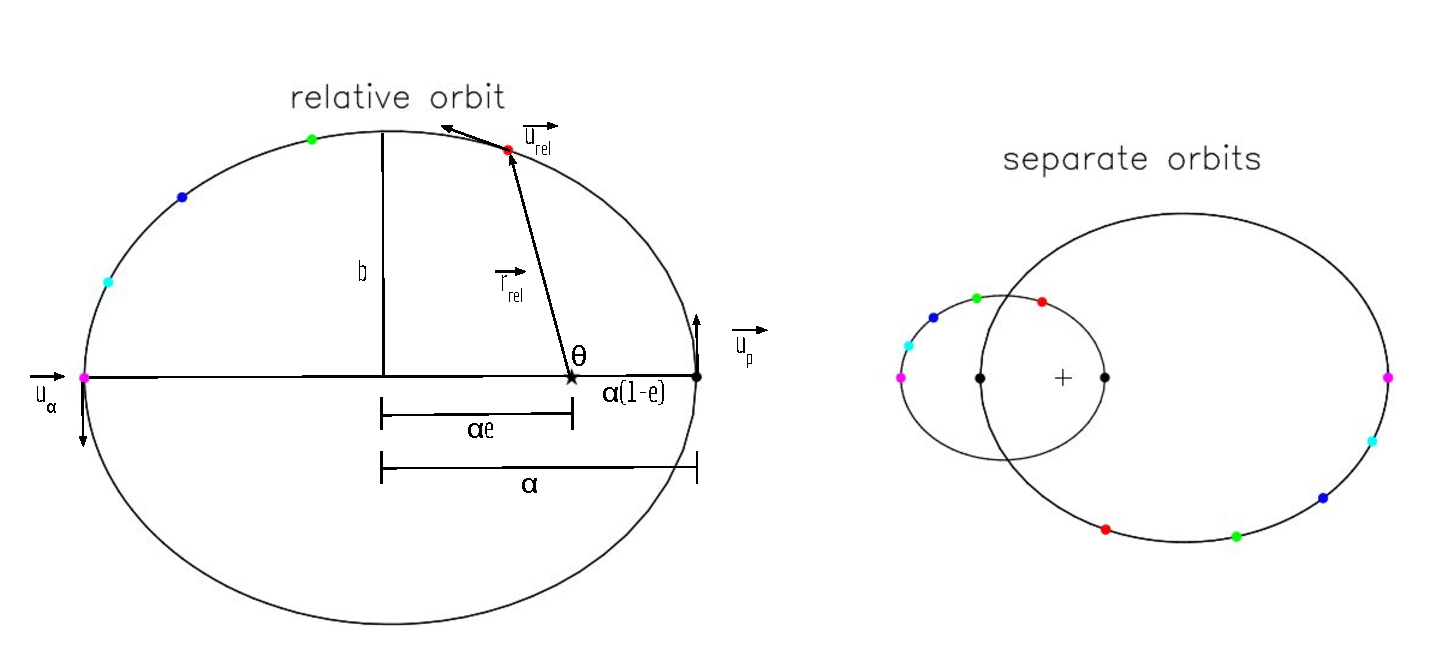
\includegraphics[width=0.9\textwidth]{Thesis/figures/relative_orbit.pdf}
    \caption{Relation between the relative orbit (left) and absolute orbits (right) of a
    binary, in this case Sirius. The black star symbol on the left figure represents the fixed star with the reference frame centered on it, while the circles represent the moving star with mass $\mu$. The absolute positions (right) are matched with the relative position of the moving body (left) via different colors.   The initial figure was taken by Frank Verbunt's lecture notes `Compact Binaries` and modified by me.}
    \label{fig:relative_orbit}
\end{figure}
The shape of the relative orbit is defined by the orbital energy and angular momentum per unit of reduced mass. For an elliptic relative orbit, specifically, the orbital energy per unit of reduced mass is
\begin{equation}\label{eq:orbital_energy}
    \epsilon = \frac{E}{\mu} = - \frac{G (M_1 + M_2)}{2\alpha}, \; \; \epsilon  < 0
\end{equation}
and the angular momentum per unit of reduced mass is
\begin{equation}\label{eq:orbital_ang_momentum}
    l = \frac{L}{\mu} = \vec{r_{rel}} \times \vec{u_{rel}} =\sqrt{G (M_1 + M_2) \alpha (1-e^2)}
\end{equation}
where $e$ is the eccentricity and $\alpha$ the semi-major axis of the eclipse, see \cref{fig:relative_orbit}. In the absence of mass loss, both $\epsilon$ and $l$ are constants of motion.  \cref{eq:orbital_energy} shows that the orbital energy is independent of the eccentricity, $e$ and in the elliptic case is always negative.

The relative position of the moving body, or the orbital separation of the binary components, see \cref{fig:relative_orbit}, is given as:
\begin{equation}\label{eq:relative_position}
    r_{rel} = \frac{\alpha (1-e^2)}{1+e \cos{\theta}}
\end{equation}
and its velocity as:
\begin{equation}\label{eq:relative_velocity}
    u_{rel}= \sqrt{GM \left( \frac{2}{r_{rel}} - \frac{1}{\alpha}\right)},
\end{equation}
where $M = M_1 + M_2$. Using \cref{eq:relative_velocity}, the semi-major axis is given as:
\begin{equation}\label{eq:semi-major_axis}
    \alpha = \frac{GM r_{rel}}{2GM - u_{rel}^2 r_{rel}}.
\end{equation}
Additionally, using  \cref{eq:orbital_ang_momentum} the eccentricity is given as:
\begin{equation}\label{eq:eccentricity}
    e = \sqrt{1 - \frac{|\vec{r_{rel}} \times \vec{u_{rel}}|^2}{G M \alpha}}.
\end{equation}

As a result, given the relative position and velocity of two stars, $M_1$ and $M_2$, the evolution of the binary can be describted using \cref{eq:orbital_energy}, \cref{eq:orbital_ang_momentum}, \cref{eq:semi-major_axis} and \cref{eq:eccentricity}.


\begin{comment}
For two stars of mass, $M_1$ at position $r_1$ and $M_2$ at position $r_2$, the the weighted mean position, namely the center of mass, can be defined as:
\begin{equation}\label{eq:center_of_mass}
    \vec{R_{cm}} = \frac{M_1 \vec{r_1} + M_2 \vec{r_2}}{M_1 + M_2}
\end{equation}
Furthermore, the reduced mass of the binary is defined as:
\begin{equation}
    \mu= \frac{M_1 M_2}{M_1 + M_2}
\end{equation}
\end{comment}


\subsection{Roche lobe overflow}\label{sub:roche_lobe}

The orbital parameters of the relative orbit are critical in defining the Roche model, a valuable tool in describing binary evolution. The Roche model describes the effective gravitational potential of the binary and it is based on three assumptions:
\begin{enumerate}
    \item The gravitational fields of both stars are assumed to be those of point masses.
    \item The binary orbit is assumed to be circular, $e=0$.
    \item The rotation of the stellar components is assumed to be synchronized with the orbital motion. 
\end{enumerate}
The Roche potential's crucial equipotential surface, which passes through the inner Lagrangian point $L_1$, defines two Roche lobes that encircle each star. Hence, each Roche lobe defines the volume in which material is gravitationally bound to the respective star. The Roche lobe can be approximated with accuracy better than $1\%$ by a sphere of radius $R_L$:
\begin{equation}\label{eq:roche_lobe}
    \frac{R_{L,1}}{\alpha} = \frac{0.49q^{2/3}}{0.6q^{2/3} + \ln{1+q^{1/3}}},
\end{equation}
where $q =M_1 / M_2$. $R_{L,2}$ is be given for $q =M_2 / M_1$. The Roche potential of a binary with $q=6.3/5.5 \approx 1.145$ and $\alpha = 1.24$ au is presented in \cref{fig:binary_equop}. The latter corresponds to the effective potential of $\xi$ Tau by replacing the inner binary masses, $M_1$ and $M_2$, with one star of mass $M = M_1 + M_2$.
\begin{figure}[H]
    \centering
    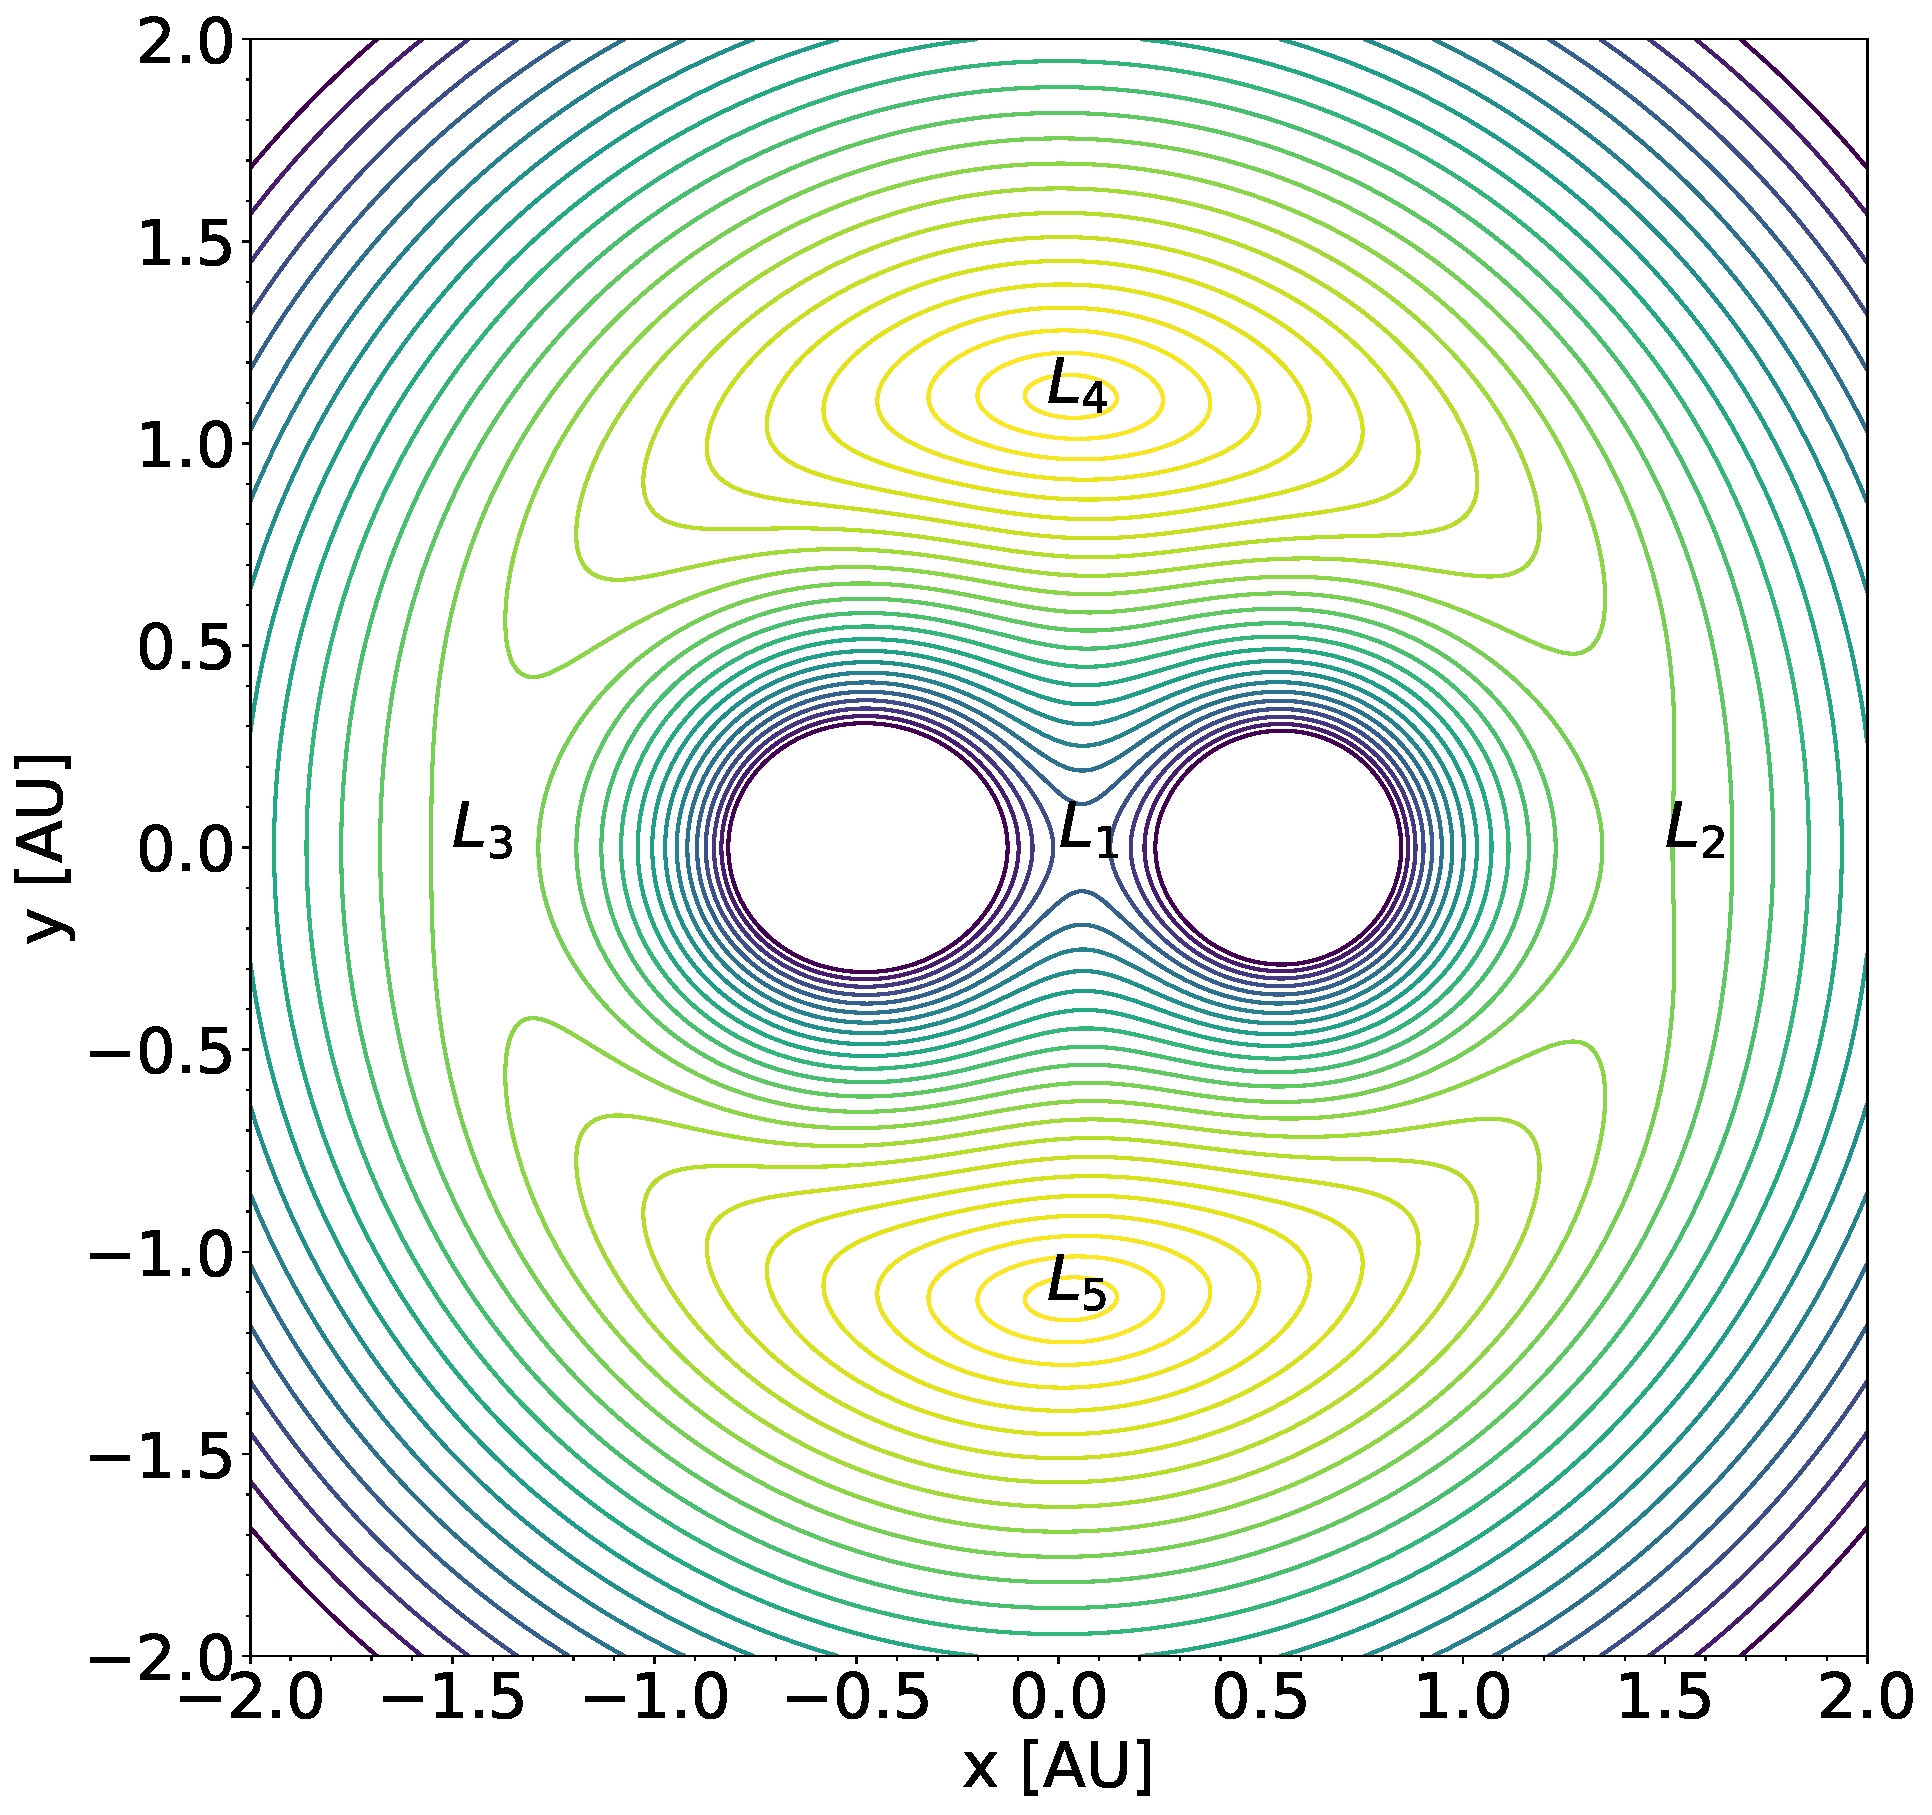
\includegraphics[width=0.9\textwidth]{Thesis/graphs/binary_equop.pdf}
    \caption{Contour plot of a binary's effective potential for $q=6.3/5.5 \approx 1.145$ and $\alpha = 1.24$ au. The five Lagrangian points are indicated as $L_1, L_2, L_3, L_4$ and $L_5$. I create the plot using the Hermite integrator which is part of AMUSE \citep{hut1995building}.}
    \label{fig:binary_equop}
\end{figure}
According to \cref{eq:roche_lobe}, the size of the Roche lobe is determined by the mass ratio $q$ and the orbital separation of the two stars, $\alpha$. The more massive star has a larger Roche lobe, whereas stars of equal mass have equal sized Roche lobes. Furthermore, the size of the Roche lobes is proportional to the orbital separation of the stars, so as the latter changes, so do the Roche lobes.

As discussed in \cref{sec:single_star_evolution}, stars contract and expand during their evolution. Additionally, the binary separation may decrease due to the loss of orbital angular momentum from the system via stellar wind mass-loss, see \cref{sub:winds} or gravitational radiation. As a result, the physical radius of a star, $R_{\star}$, may become larger than its Roche lobe radius, $R_{L}$. This scenario is called Roche-lobe overflow (RLOF) and matter from the outer layers of the Roche-lobe-filling star can freely move through the first Lagrangian point $L_1$ to the companion star. 


Mass flow via the $L_1$ point is a relatively complicated hydrodynamical problem, but the rate of mass transfer, $\dot{M}$, through $L_1$ is highly sensitive to the donor's fractional radius excess, $\frac{\Delta R}{R}$ . A comprehensive derivation of Bernoulli's law to the gas flow through the nozzle near $L_1$ results in 
\begin{equation}\label{eq:mass_loss_rate_anal}
    \dot{M} \propto \frac{M_{d}}{P} \left( \frac{\Delta R}{R}\right)^3,
\end{equation}
where $M_{d}$ is the donor mass and $P$ the orbital period of the binary.
\begin{comment}
    

Hence, the timescale of mass transfer is strongly dependent on the donor's fractional radius excess:
\begin{equation}\label{eq:mass_transfer_timescale}
   \frac{\Delta R}{R} \propto \frac{P}{t_{\dot{M}}}^{1/3}
\end{equation}
\end{comment}

According to \cref{sec:single_star_evolution}, intermediate-mass stars expand during MS on nuclear timescale and during RGB and AGB phases, on thermal timescale, see \cref{fig:HR_evolution}.  Hence, three cases of mass transfer can be distinguished:
\begin{enumerate}
    \item During the MS, namely Case A
    \item During post-MS and before helium exhaustion, namely Case B
    \item After helium exhaustion, namely Case C
\end{enumerate}
Considering that mass is the most important property for a star's evolution, see \cref{sec:single_star_evolution}, RLOF can significantly alter its evolutionary outcome. Thus, in a mass-transferring binary system, both stars are expected to deviate from the evolutionary paths they would have in the absence of mass transfer. 

\subsection{Orbital evolution during mass transfer}\label{sub:orbit_evol_mass_loss}

During mass transfer, the transferring matter carries angular momentum causing the orbital parameters of the relative orbit to change. By differentiating Eq. \eqref{eq:orbital_ang_momentum}, a general equation for the orbital evolution can be obtained:
\begin{equation}\label{eq:orb_ang_momen_derivative}
    2\frac{\dot{J}}{J} = \frac{\dot{\alpha}}{\alpha} + 2 \frac{\dot{M_1}}{M_1} + 2 \frac{\dot{M_2}}{M_2} - \frac{ \dot{M_1} + \dot{M_2}}{M_1 + M_2} - \frac{2e \dot{e}}{1-e^2},
\end{equation}
where the last term vanishes for circular orbits.

A basic assumption of \cref{eq:orb_ang_momen_derivative} is that the angular momentum stored in the rotation of the two stars is negligible compared to the orbital angular momentum. In most circumstances, this assumption is valid, however in the case of rapidly spinning objects, such as millisecond pulsars, the angular momentum contained in the pulsar's rotation may need to be considered.  

From \cref{eq:orb_ang_momen_derivative}, the evolution of the semi-major axis of the relative orbit during mass loss is given as:
\begin{equation}\label{eq:semimajor_axis_derivative}
     \frac{\dot{\alpha}}{\alpha} = 2\frac{\dot{J}}{J} - 2 \frac{\dot{M_1}}{M_1} - 2 \frac{\dot{M_2}}{M_2} + \frac{ \dot{M_1} + \dot{M_2}}{M_1 + M_2} + \frac{2e \dot{e}}{1-e^2},
\end{equation}
where the variable $\dot{J}$ represents angular momentum loss from the binary. 

The mass loss can be simply parameterized as
\begin{equation}\label{eq:mass_loss_non_cons}
    \dot{M_{a}} = - \beta \dot{M_{d}},
\end{equation}
where the subscript $a$ refers to the `accretor` and $d$ to the `donor`. In this case, $\beta$ is the fraction of the transferred mass that is accreted by the companion, and thus
\begin{equation}\label{eq:mass_loss_non_cons_2}
    \dot{M_{a}} + \dot{M_{d}} = (1-\beta) \dot{M_{d}}.
\end{equation}

In the ideal situation where all the transferred mass from the first star is accreted by the second, $\beta=1$, the orbital angular momentum of the binary is conserved, $\dot{J}=0$ and \cref{eq:semimajor_axis_derivative} reduces to
\begin{equation}\label{eq:orb_ang_momen_derivative_cons}
    \frac{\dot{\alpha}}{\alpha}= 2 \left( \frac{M_d}{M_a} - 1 \right) \frac{\dot{M_{d}}}{M_{d}} + \frac{2e \dot{e}}{1-e^2}.
\end{equation}    
This the case of conservative mass transfer and a close look to \cref{eq:orb_ang_momen_derivative_cons} reveals that for a circular orbit the orbital separation shrinks as long as $M_d > M_a$, while it expands when $M_d < M_a$. Finally, the minimum orbital distance is given for $M_d = M_a$. 

In the general case of RLOF, mass transfer is expected to be non-conservative meaning that  $\beta < 1$. Furthermore,
the ejected mass carries away orbital angular momentum from the system. The amount of specific angular momentum that is lost can be parameterized to be $\eta$ times the specific angular momentum of the binary:
\begin{equation}\label{eq:orb_ang_mom_non_cons}
    \frac{\dot{J}}{J} = \eta \frac{\dot{M_{a}} + \dot{M_{d}}}{M_{a} + M_{d}}.
\end{equation}
Using \cref{eq:mass_loss_non_cons_2} and \cref{eq:orb_ang_mom_non_cons}, \cref{eq:semimajor_axis_derivative} gives:
\begin{equation}\label{eq:orb_ang_momen_derivative_non_cons}
    \frac{\dot{\alpha}}{\alpha}= -2\frac{\dot{M_{d}}}{M_{d}} \left( 1- \beta\frac{M_d}{M_a} - (1-\beta)(\eta + \frac{1}{2}) \frac{M_d}{M_d + M_a}  \right)  + \frac{2e \dot{e}}{1-e^2}.
\end{equation}  
The parameters $\beta$ and $\eta$ are highly uncertain. Depending on the mass transfer mode, $\eta$ can be specified in terms of other quantities \citep{postnov2014evolution}.

Assuming circular orbit, $\beta$ and $\eta$ to be constants and by ignoring the internal angular momentum of the stars, \cite{portegies1995formation} shows that the evolution of the semi-major axis based on mass redistribution can be described as:
\begin{equation}\label{eq:semimajor_axis_no_cons}
    \frac{\alpha}{\alpha_{0}} = \left (\frac{M_{d} M_{a}}{M_{d,0} M_{a,0}} \right)^{-2} \left (\frac{M_{d} + M_{a}}{M_{d,0}+M_{a,0}} \right)^{2\eta +1},
\end{equation}    
where the `0` subscript corresponds to the initial values, before RLOF.
    






\section{Hierarchical triple star systems}\label{sec:triples_evolution}

The majority triple star systems are observed in hierarchical structures. More specifically, they consist of an inner binary and a distant star (hereafter tertiary/outer star) that orbits the center of mass of the inner binary system such as $\frac{\alpha_{in}}{\alpha_{out}} << 1$. A schematic of a hierarchical triple system is presented in \cref{fig:triple_schem}.
\begin{figure}[H]
    \centering
    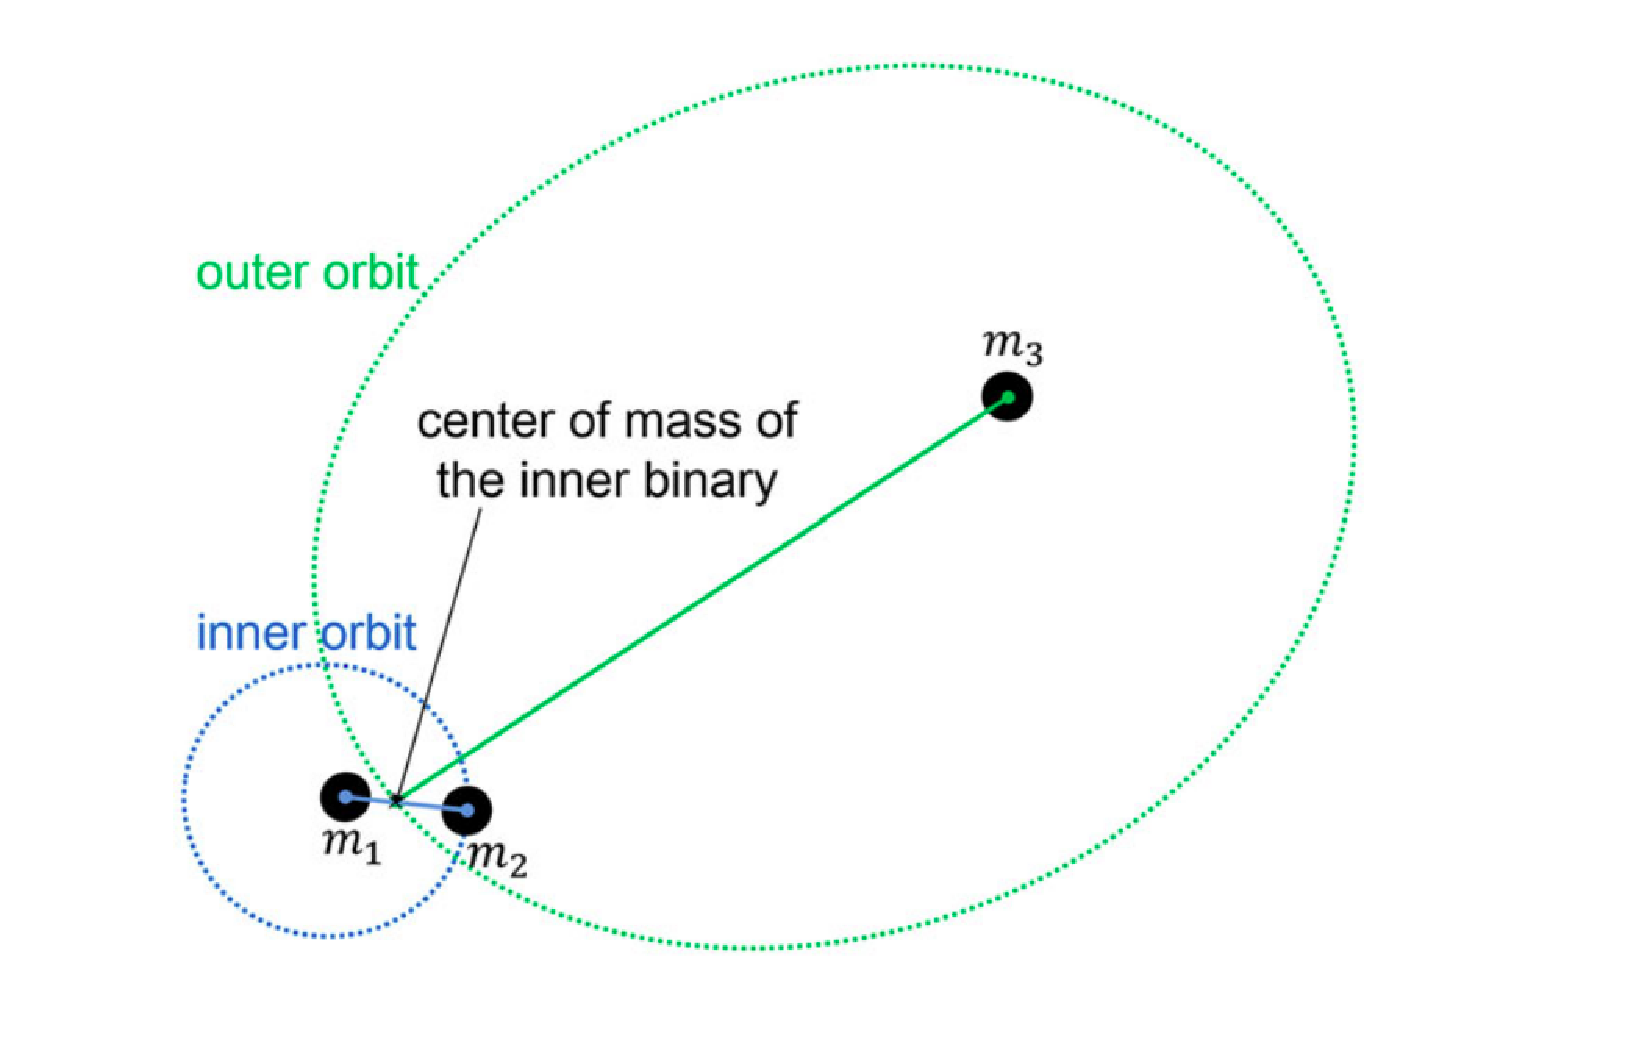
\includegraphics[width=0.9\textwidth]{Thesis/figures/triple_schem.pdf}
    \caption{A schematic of a hierarchical triple system consisting of an inner and an outer binary. The inner binary consists of objects whose masses are $m_1$ and $m_2$, and the outer one is the pair of the inner binary and the third body with mass $m_3$. Figure taken by \cite{gupta2020gravitational}.}
    \label{fig:triple_schem}
\end{figure}
In certain situations, the presence of the outer star does not alter the evolution of the inner binary. In such cases, the evolution of the tertiary  and the inner binary can be studied separately. In other circumstances, the three stars interact in ways that are unique to systems with multiplicities higher than binaries. As a result, numerous new evolutionary paths are anticipated compared to binary evolution. In the following subections, I focus on the dynamical stability of triple systems and the Lidov-Kozai cycles. These topics are relevant to my work, but for a detailed overview of triple evolution I direct the reader to \cite{michaely2014secular,toonen2016evolution}.

\subsection{Stability of triples}\label{sub:stability_triples}

Unlike two-body systems, the three-body problem does not have closed-form solutions. On the one hand, triple systems in the unstable regime tend to disintegrate into lower order systems on dynamical timescales \citep{van2007formation}. On the other hand, stability can occur (and last) on different timescales, thus it is not trivial to draw a clear line between stable and unstable triple systems. 

\cite{mardling1999dynamics} stability criterion is usually used in studies of triple systems' evolution, where a system is unstable if
$\frac{\alpha_{in}}{\alpha_{out}} < \frac{\alpha_{in}}{\alpha_{out}} |_{crit}$. The critical fraction is given as:
\begin{equation}\label{eq:stability_regime}
    \frac{\alpha_{in}}{\alpha_{out}} |_{crit} = \frac{2.8}{1-e_{out}} (1- \frac{0.3 i_{mut}}{\pi}) \left ( \frac{(1 + q_{out})(1+e_{out})}{\sqrt{1-e_{out}}} \right )^{2/5},
\end{equation}
where $q_{out} \equiv m_3 / (m_1 + m_2)$. The criterion is based on the concept of chaos and the result of overlapping resonances. The criterion is conservative since the existence of chaos is not always synonymous with instability. Many more stability criteria have been proposed and I direct the reader to \cite{mardling2001stability,georgakarakos2008stability}.

In \cref{sub:orbit_evol_mass_loss} I discussed how the orbital parameters change during non-conservative mass transfer. These concepts are also applicable for triples, where the orbital parameters of the inner and the outer orbit can change due to angular momentum loss from the system. As a result, initially stable triple systems can become dynamically unstable during their evolution.

\subsection{Lidov-Kozai cycles}\label{sub:lidov_kozai}

Dynamical interactions in hierarchical triples can differ from the case of binaries. The presence of the third star can give rise to the Lidov-Kozai mechanism \citep{lidov1962evolution,kozai1962secular}, which can have a significant impact on the secular evolution the system. During Lidov-Kozai cycles, the mutual torque between the inner and outer binary orbits result to angular momentum exchange. Furthermore, the orbital energy is preserved, and hence the semi-major axes are also conserved. Consequently, the orbital inner eccentricity and mutual inclination vary periodically (i.e. 'cycles'). When the inclination between the two orbits is minimized, the inner binary's eccentricity reaches its maximum. Furthermore, the pericenter argument may rotate or librate periodically.

Evolution during Lidov-Kozai cycles can be fairly complicated, but given some assumptions, analytical expressions can be derived. For example, in the test-particle approximation ($e_{in}=e_{out}=0$ and $M_2 << M_1, M_3$ \citep{naoz2013secular}), the mechanism is expected to take place only if $i_{mut} \in [39.2^{\circ},140.8^{\circ}$]. Furthermore, by expanding the three-body Hamiltonian to quadrupole order in $a_{in}/a_{out}$ \citep{kinoshita1999analytical}, the timescale for the Lidov-Kozai cycles is
\begin{equation}\label{eq:lidov_kozai_timescale}
    t_{kozai} \approx \frac{P_{out}^2}{P_{in}} + \frac{M_1 + M_2 +M_3}{M_3}(1-e_{out}^2)^{3/2},
\end{equation}
where $P_{in}$ and $P_{out}$ are the periods of the inner and outer orbit, respectively. Typically, $t_{kozai} >> P_{in},P_{out}$.

Higher orders of $a_{in}/a_{out}$, i.e. the octupole level of approximation, result to even richer dynamical behavior than the quadrupole approximation. The octupole term is expected to be important when $\epsilon_{oct} \geq 0.01$ \citep{naoz2011hot,shappee2013mass} and
\begin{equation}\label{eq:octupole_term}
    \epsilon_{oct} = \frac{M_1 - M_2}{M_1 + M_2} \frac{a_{in}}{a_{out}} \frac{e_{out}}{1-e_{out}^2}.
\end{equation}

\section{Scientific Codes}\label{sec:scientific_codes}

In this section, I introduce the scientific codes that I coupled together in order to simulate the evolution of my target system.  Because these codes can be used in a variety of astrophysical scenarios, I will concentrate on their fundamental usage and working principles. I encourage users who want to dig deeper into the codes to follow the relevant citations. 

\subsection{MESA}

MESA (Modules for Experiments in Stellar Astrophysics, \cite{paxton2010modules,paxton2013modules,paxton2015modules,paxton2019modules}) is a powerful and versatile 1D stellar evolution code that has become one of the most widely used tools in modern astrophysics. The code is written in Fortran and is designed to solve the fully coupled structure and composition equations simultaneously, allowing for highly accurate models of stars.

MESA includes a wide range of physics modules for various astrophysical processes, such as the equation of state, nuclear reaction networks, hydrodynamics, convective and radiative energy transport, mass loss, rotation, and magnetic fields. The code can simulate the evolution of stars from their birth to their death, including complex phases such as helium and carbon burning, thermal pulses, and supernova explosions. As a result, MESA is an invaluable tool for astrophysical research, from studying the formation and evolution of stars to exploring the origins of the elements in the universe.

The central feature of MESA is the solution of the coupled structure and composition equations, which describe the internal structure of stars and the evolution of their chemical composition over time. These equations are based on fundamental principles of stellar physics, such as conservation of mass, momentum, and energy, as well as nuclear reactions that generate and consume energy in the star. The structure and composition equations can be written as a set of coupled differential equations that describe the evolution of the mass, radius, luminosity, temperature, and chemical composition of the star over time \citep{paxton2010modules,paxton2013modules,paxton2015modules,paxton2019modules}).

MESA also includes a comprehensive nuclear reaction network that describes the fusion of light elements into heavier elements in the stellar core. The network includes thousands of nuclear reactions that involve hundreds of isotopes, making it one of the most detailed and accurate nuclear reaction networks available for stellar evolution calculations.


\subsection{GADGET-2}\label{sub:gadget2}

A detailed documentation of GADGET-2 is out of the scope of this section. Nevertheless, GADGET-2, is the main code used in my simulations, thus the general description of the code will be followed by the basic principles behind the calculation of hydro- and collisionless dynamics.

GADGET-2 (GAlaxies with Dark matter and Gas intEracT) is a smoothed particle hydrodynamics (SPH) code that simulates the gravitational and hydrodynamic evolution of collisionless and gaseous systems in astrophysical contexts \citep{springel2005cosmological}. The code is capable of modeling a wide range of physical processes, such as gas dynamics, gravity, magnetic fields, and radiative transfer. GADGET-2 is written in C++ and is publicly available under the GNU General Public License.

The hydrodynamics computation in GADGET-2 is performed by solving the equations of motion for each particle in the simulation domain. The acceleration of each particle is calculated by summing the forces acting on it, including gravity, pressure gradients, and artificial viscosity. The gravity calculation uses the hybrid TreePM method \citep{bode2000tree,bagla2002treepm}, where the simulation volume is recursively subdivided into cubic cells, with each cell containing a maximum number of particles. The algorithm then builds a tree structure where each cell is treated as a node, and nodes that are spatially close are grouped together to form larger nodes. The final tree structure is used to compute the gravitational force on each particle avoiding the need to calculate the force between all pairs of particles in the system. This method reduces the computational cost from $O(N^2)$ for direct summation to $O(N\log N)$, where $N$ is the number of particles.

The code also includes modules for modeling magnetic fields and radiative transfer. The magnetic field module includes algorithms for calculating the magnetic field evolution and its effects on the gas dynamics. The radiative transfer module includes algorithms for calculating the transport of radiation through the simulation domain and its effects on the gas and dust properties. GADGET-2 can be run in parallel on high-performance computing clusters using the Message Passing Interface (MPI) standard.

\subsubsection{Hydrodynamics}

The basic principle of the SPH method is that the fluid is represented as a set of particles with associated physical attributes such as density, pressure, and velocity. These properties are calculated at a given point in space, using the interpolation method. The method allows any function to be defined in terms of its values at a group of disordered points known as particles \citep{monaghan1982particle}. The integral interpolant of any function $f(r)$ is defined by:
\begin{equation}\label{eq:interpolant}
    \langle f(r) \rangle = \int f(r') W(r-r',h) dr'
\end{equation}
where the integration is performed across the entire space and $W$ is an interpolating/smoothing kernel. Furthermore, the method is Lagrangian, meaning that the particles move with the fluid and do not have a fixed position in space.

The smoothing kernel has two basic properties, similar with Dirac's delta function:
\begin{equation}\label{eq:kernel_property_1}
    \int W(r-r',h) dr' = 1
\end{equation}
and
\begin{equation}\label{eq:kernel_property_2}
   \lim_{h\to0} W(r-r',h) = \delta(r-r').
\end{equation}

GADGET-2 code uses the cubic spline kernel of \cite{monaghan1985refined}:
\begin{equation}\label{eq:spline_kernel}
  W(|r|,h) = \frac{1}{\pi h^3}
    \begin{cases}
      1 - \frac{3}{2}q^2 + \frac{3}{4}q^3, & 0 \leq q < 1\\
      \frac{1}{4}(2 - q)^3, & 1 \leq q <2 \\
      0, &  q \geq 2,
    \end{cases}      
\end{equation}
where $q = \frac{r}{h}$. The kernel is smooth and has a compact support, meaning it averages the properties of neighboring particles within a certain radius, called smoothing length, $h$, of the target point.  

When $q \geq 2$, there is no interaction, since $W(|r|,h)$ is zero. Thus, the amount of interactions for each particle is determined by the smoothing length $h$. When $h$ is too small, there aren't enough particles to interact with, resulting in poor precision. When $h$ is too large, local characteristics are scattered out too much, resulting in low precision and sluggish computation. Hence, the selection of the smoothing kernel, as well as an appropriate smoothing duration, is critical for both accuracy and speed. 

To make the most of SPH's Lagrangian nature, one must accommodate for an adaptive $h$. The smoothing length should be small in high-density regions and large in low-density regions. For example, the density estimate,  which GADGET-2 does is in the form of:
\begin{equation}
    \rho_i = \sum_{j=1}^{N} m_j W(r_i -r_j,h_i),
\end{equation}
where adaptive smoothing lengths $h_i$ of each particle are designed in such a way that their kernel volumes contain a constant mass for the estimated density, implying that the smoothing lengths and estimated densities follow the (implicit) equations
\begin{equation}
    \frac{4\pi}{3} h_{i}^3 \rho_i = N_{sph} \bar{m}
\end{equation}
where $N_{sph}$ is the typical number of smoothing neighbours, and $\bar{m}$ is an average particle mass. In my simulations, I use the default value $N_{sph}=50$. 

\begin{comment}
When two gas particles approach each other the contribution of viscosity in their equation of motion cannot be ignored. Viscosity results to the transfer of momentum along velocity gradients by random motions of
the gas. To account for that, GADGET-2 (and SPH codes in general) adopts an artificial viscosity scheme.
\end{comment}


\subsubsection{Collisionless dynamics}

In self-gravitating SPH codes such as GADGET-2, the point particles represent a large amount of mass and may get arbitrarily and abnormally near in a simulation, and numerical rounding may blow up. In order to avoid particles from scattering too strongly off of one another on close approach, a softening kernel, is used to also soften gravitational forces. 

\begin{figure}[H]
    \centering
    \includegraphics[width=0.9\textwidth]{Thesis/figures/smoothening.pdf}
    \caption{The functional form of the modified potential (-), gravitational force and the density profile using the cubic spline kernel. Figure taken by \cite{price2007energy}.}
    \label{fig:smoothened_gravity}
\end{figure}

GADGET-2 employs once again the cubic spline kernel, Eq. \eqref{eq:spline_kernel}, where now $h$ refers to the softening lenght. In general the softening length can differ from the smoothing length used in the hydrodynamic calculations, but in my simulations they are equal. The basis for this is \cite{bate1997resolution} study, which demonstrated that in self-gravitating SPH simulations, employing a softening length that differs from the smoothing length might lead in unphysical results. Hence, the modified gravitational potential per unit mass is given as:
\begin{equation}\label{eq:softened_gravity}
   \Phi(r) = -G\sum_{i=1}^{N} m_i W(r-r_i,h)
\end{equation}


The functional form of the modified potential, gravitational force and the density profile using the cubic spline kernel is depicted in \cref{fig:smoothened_gravity}. It is apparent that, for $q \geq 2$, the softening is zero and the potential follows the exact form, $\Phi(r) \propto -\frac{1}{r}$. 

\subsection{Huayno}\label{sub:huayano}

Huayno \citep{pelupessy2012n} is a high-performance N-body integrator code designed to simulate the dynamics of collisionless systems, such as galaxies, star clusters, and dark matter halos. The code is written in C++ and the basic principle of Huayno is the use of a hybrid algorithm \citep{bode2000tree} that combines the particle-mesh (PM) \citep{klypin1983three} and tree-based algorithms \citep{barnes1986hierarchical,dehnen2000very} to reduce the computational cost of simulating large systems.


The PM algorithm represents the gravitational potential as a discrete mesh of fixed resolution, and the particle positions are interpolated onto the mesh using a cloud-in-cell (CIC) scheme. The gravitational forces are then calculated by solving Poisson's equation on the mesh. The tree-based algorithm, on the other hand, uses a hierarchical structure to group particles into clusters and calculates the forces between clusters at different levels of the hierarchy. By combining the advantages of both algorithms, Huayno can handle a wide range of particle distributions and non-equilibrium systems, such as systems with binary or multiple stars.






\chapter{Methods}\label{methods}

\epigraph{The universe must be full of voices, calling from star to star in a myriad tongues. One day we shall join that cosmic conversation}{Arthur C. Clarke}

In order to simulate the evolution of hierarchical triple-star systems with a  Roche-lobe-filling outer star, various physical processes, such as stellar evolution, gravitational dynamics, and hydrodynamics needs to be considered. First, I employ the stellar evolution code MESA \citep{paxton2010modules,paxton2013modules,paxton2015modules,paxton2019modules} to model the evolution of the system's stars prior to outer stars' \ac{rlof}. Once the outer star reaches the stage where it approximately fills its Roche lobe, I pause the stellar evolution simulation and convert the one-dimensional stellar structure into a three-dimensional hydrodynamical model. This 3D hydrodynamical model of the outer star is then relaxed, using GADGET-2 \citep{springel2005cosmological}, and placed in orbit around the binary star. The inner binary components are seen as point masses and their gravitational dynamics are handled by Huayno \citep{pelupessy2012n}. Subsequently, I monitor the intricate hydrodynamics of the mass transfer from the Roche lobe-filling outer star to the inner binary for multiple orbits, while simultaneously keeping track of the three stars gravitational dynamics and the outer star gas hydrodynamics. In this chapter I present in detail all the aforementioned steps. In each step I discuss the exploration of different parameters, the underlying assumptions of the models and their physical justification.

\section{Stellar evolution}\label{sec:stellar_evolution}

The stellar evolution calculations in this work are performed using the normal AMUSE parameters for MESA, with solar metallicity as the input.
MESA allows me to track the independent evolution of the triple system components and obtain estimations of their properties at the beginning of RLOF. In this work, I allow the tertiary to evolve until $R_{stop} = 1.1 \times R_{L}$, see \cref{eq:roche_lobe}. The consequence of this choice will be discussed in detail in \cref{simulations}.

By the time the outer star approaches the radius of its Roche lobe, all three stars have lost some mass, while the tertiary's radius is much bigger than when it was formed. In order to accurately evaluate the Roche lobe sizes,  I need to estimate the masses of the stars at the RLOF moment. Unfortunately, $\xi$ Tau's age is not known, but mass-loss via winds during the main sequence is expected to be unimportant for low- and intermediate- mass stars, see \cref{sub:winds}.

Despite that, I track the evolution of the tertiary's mass and radius profile. As expected, radiation-driven mass-loss proved negligible in this mass regime. For cold winds, I utilize Reimer's, see Eq. \eqref{eq:reimer}, and Blocker's, see Eq. \eqref{eq:blocker}, mass-loss prescriptions using commonly used scaling factors of $\eta = 0.5$ and $\eta = 0.1$, respectivelly. 
\begin{figure}[H]
    \centering
    \begin{subfigure}{.5\textwidth}
    \centering
    \includegraphics[width=0.9\textwidth]{Thesis/graphs/giant_1-1mass_loss.pdf}
    \label{fig:mass_loss}
    \end{subfigure}%
    \begin{subfigure}{.5\textwidth}
    \centering
    \includegraphics[width=0.9\textwidth]{Thesis/graphs/giant_1-1radius.pdf}
    \label{fig:radius_profile}
    \end{subfigure}
    \caption{ Mass and radius evolution of a 5.5 M$_{\odot}$ star at solar metallicity until RLOF. ZAMS and TAMS are noted by black circles, while the start and end of helium burning by black squares. I create the stellar evolution models using MESA \citep{paxton2010modules,paxton2013modules,paxton2015modules,paxton2019modules}.}
\end{figure}
The tertiary loses less than $1\%$ of its 
initial mass, while the expected mass-loss from the binary components is even smaller, because less massive, and thus less luminus, stars will have weaker winds. As a result, I do not correct for mass-loss and use the parameters listed in  \cref{tab:system_orbit_param}.  

At this point, I also assume that the mass lost through winds has no effect on the stars. This assumption would be false in the case of more massive stars. As mass escapes from the star's surface, it carries angular momentum and can change the inner and outer orbital parameters. Furthermore, some of the escaped mass can be accreted, complicating the evolution of the two orbits even further. Given the small amount of mass loss, the aforementioned assumption is safe in this case.

In \cref{fig:HR_ROLF}, I present the evolution of the tertiary on the HR diagram until the moment of RLOF and in \cref{tab:tertiary_param_ROLF} I summarize the tertiary's important stellar parameters. 
\begin{figure}[H]
    \centering
    \includegraphics[width=0.9\textwidth]{Thesis/graphs/HR_1-1ROLF.pdf}
    \caption{Evolution of 5.5 M$_{\odot}$ at solar metallicity until the moment of RLOF. ZAMS and TAMS are noted by black circles, while the start and end of helium burning by black squares. The evolutionary phases have categorized in different colors similar to \cref{fig:HR_evolution}. I calculate the track using MESA \citep{paxton2010modules,paxton2013modules,paxton2015modules,paxton2019modules}. The dashed lines show lines of constant radii by means of the Stefan–Boltzmann law.}
    \label{fig:HR_ROLF}
\end{figure}
\begin{table}[H]
    \centering
    \begin{tabular}{| c | c |}
       Parameter & Value \\
       \hline 
       M$_{RLOF}$ & 5.5 (M$_{\odot}$) \\
       R$_{RLOF}$ & 91.36 (R$_{\odot}$) \\
       L$_{RLOF}$ & 2262 (L$_{\odot}$) \\
       t$_{RLOF}$ & 82.36 (Myr) 
    \end{tabular}
    \caption{ $\xi$ Tau parameters at the beginning of RLOF. From top to bottom the tertiary's mass, radius, luminosity and age.}
    \label{tab:tertiary_param_ROLF}
\end{table}
The tertiary is expected to overflow its Roche lobe during the early AGB phase, after helium exhaustion, leading to a type C mass transfer. Hence, I expect that the envelope will be convective, see \cref{sec:single_star_evolution}.

In order to verify that, I present a Kippenhahn diagram of the tertiary, see \cref{fig:kippen_plot}. This diagram displays the structural evolution of the star from the core to the photosphere. The vertical axis represents the position within the star in terms of enclosed mass and the horizontal axis represents the number of the models, which are translated to stellar age (hence the x-axis is not linear). In this diagram, one can see how different regions are discerned: The white parts are the radiative regions, the stripped parts represent the convective regions, and the variation of the color represent the intensity of the energy generation at various regions in arbitrary units. Darker color indicate that more energy is produced.
\begin{figure}[H]
    \centering
    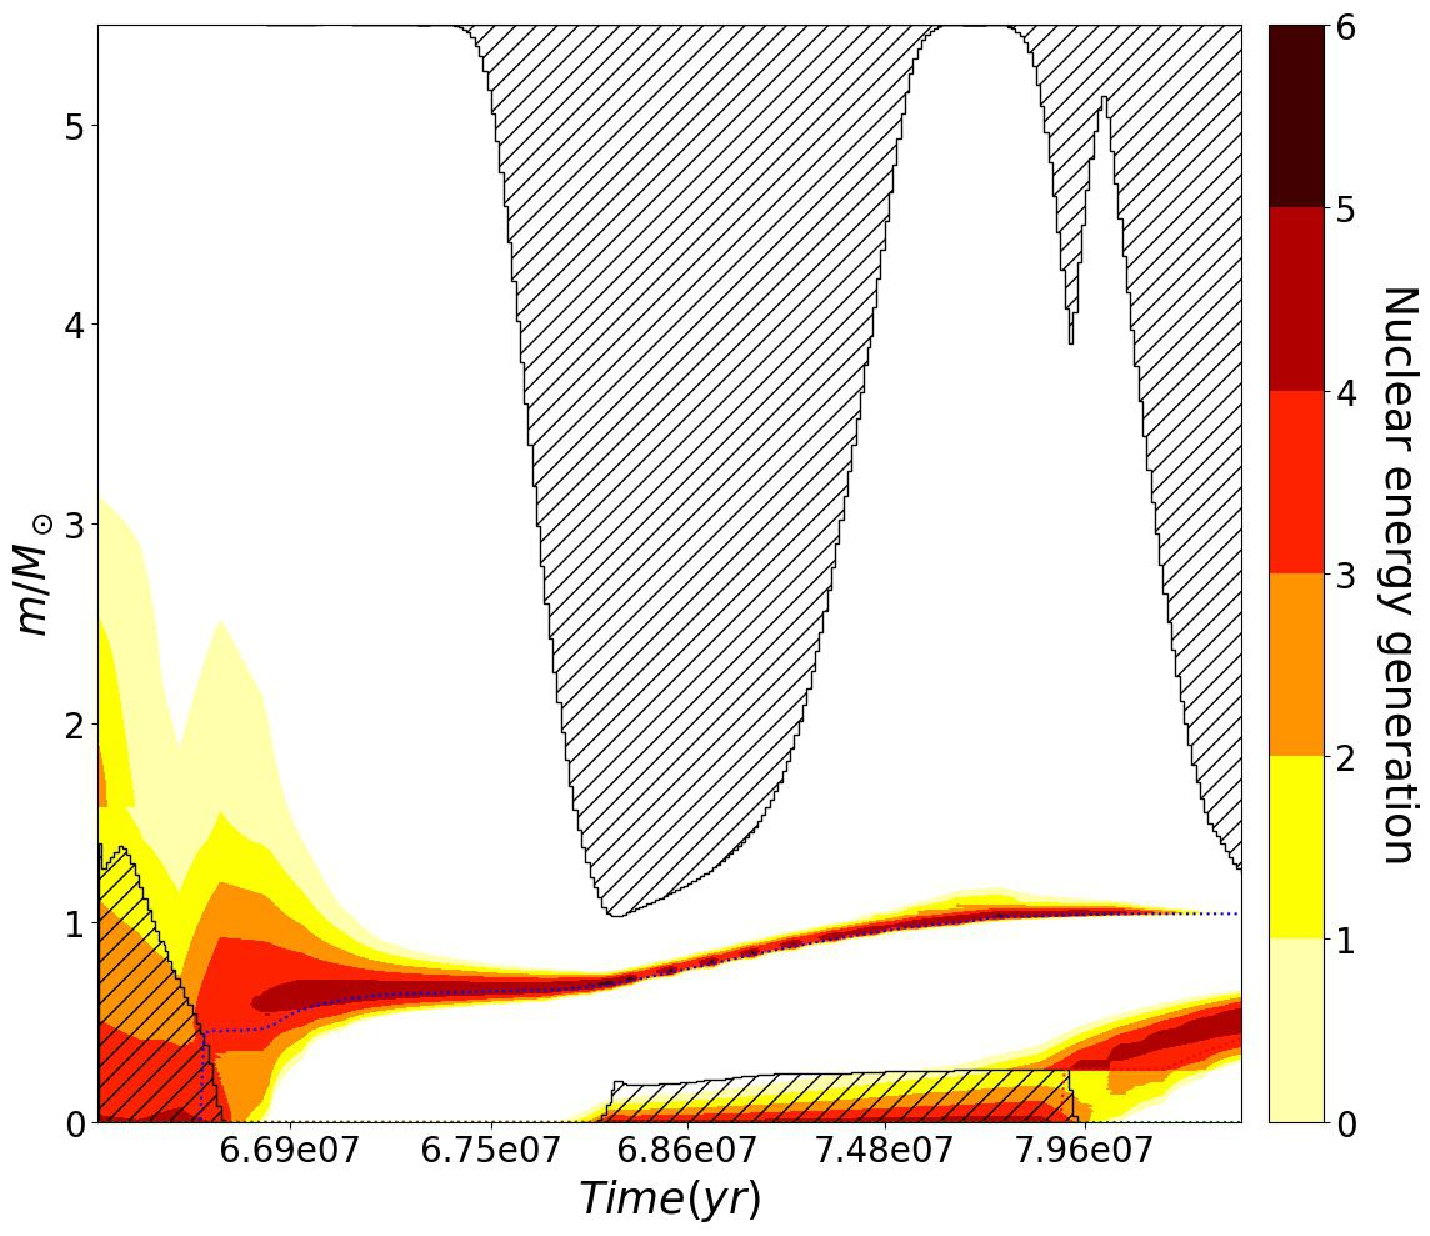
\includegraphics[width=0.9\textwidth]{Thesis/graphs/Kippen_ROLF_Schw.pdf}
    \caption{Kippenhahn diagram of $\xi$ Tau outer component until the onset of RLOF using Schwarzwild criterion, see Eq. \eqref{eq:Schwarzwild_criterion}. The vertical axis represents the position within the star in terms of enclosed mass and the horizontal axis represents the number of the models which are translated to stellar age. The white parts are radiative regions, the stripped parts represent convective regions, and the variation of the color represent the intensity of the energy generation at various regions in arbitrary units. Darker color indicate that more energy is produced. I create the graph using MESA \citep{paxton2010modules,paxton2013modules,paxton2015modules,paxton2019modules}.}
    \label{fig:kippen_plot}
\end{figure}
At the moment of RLOF, the convective envelope has penetrated deep inside the star close to the actual core. Hence, in this case, convection defines the mechanical structure of the envelope. This is critical for the 3D hydrodynamical model and it is discussed in detail in \cref{sec:1D_to_3D}. 

Given the parameters in \cref{tab:tertiary_param_ROLF}, I also calculate the relevant characteristic timescales of the tertiary, see \cref{sec:timescales}, which are listed in \cref{tab:tertiary_timescale_ROLF}.
\begin{table}[H]
    \centering
    \begin{tabular}{| c | c |}
       Timescale & Duration \\
       \hline
       $t_{dyn}$ & 4.85 day\\
       $t_{th}$ & 4585.78 yr 
    \end{tabular}
    \caption{ Tertiary timescales at the beginning of RLOF.}
    \label{tab:tertiary_timescale_ROLF}
\end{table}
\begin{comment}
In \cref{tab:system_orbit_param_ROLF} I summarize the important parameters of the system at the moment of RLOF. 
\begin{table}[H]
    \begin{adjustbox}{width=1\textwidth}
    \small
    \centering
    \begin{tabular}{| c c c c c c c c c c|}
       M$_1$ (M$_{\odot}$) & 
       M$_2$ (M$_{\odot}$) &
       M$_3$ (M$_{\odot}$) & $\alpha_{in}$ (au) &
       $\alpha_{out}$ (au) &
       $\epsilon_{in}$ &
       $\epsilon_{out}$ &
       $R_{RLOF}$ (au) &
       $t_{RLOF}$ (Myr) &
       $M_{RLOF}$  (M$_{\odot}$) \\
       \hline
       3.2 & 3.1 & 5.5 & 0.133 & 1.24 & 0.0 & 0.15 & 0.423 & 82.36 & 5.5
    \end{tabular}
    \end{adjustbox}
    \caption{ Orbital parameters of $\xi$ Tau system at the beginning of RLOF}
    \label{tab:system_orbit_param_ROLF}
\end{table}
Given these parameters, I also calculate the relevant characteristic timescales of the tertiary, which are listed in \cref{tab:tertiary_timescale_ROLF}.
\begin{table}[H]
    \centering
    \begin{tabular}{| c | c |}
       Timescale & Duration \\
       \hline
       $t_{dyn}$ & 4.85 day\\
       $t_{th}$ & 4585.78 yr 
    \end{tabular}
    \caption{ Tertiary timescales at the beginning of RLOF.}
    \label{tab:tertiary_timescale_ROLF}
\end{table}
\end{comment}
Note that the default parameters of MESA withing AMUSE do not include overshooting. However, I perform one test taking into account overshooting with $f=0.016$ \citep{herwig2000evolution}. On one hand, the MS lifetime extends, RLOF occurs $~10Myr$ later in the evolution, while the stellar core is more massive. On the other hand, the impact on the structure of the envelope's outer layers at the moment of RLOF is negligible. This is the region of highest interest for my mass transfer simulations, thus I proceed with models without overshooting. Nevertheless, it is worth mentioning that for $f=0.016$, RLOF occurs before helium exhaustion leading to a type B mass transfer.

\section{Converting the 1D stellar evolution model to a 3D gas particle distribution}\label{sec:1D_to_3D}

In addition to fundamental parameters such as mass, radius, etc., MESA enables to access the stars internal structure. This information is essential to convert the 1D stellar models into 3D hydrodynamical realizations, providing a more comprehensive understanding of the physical processes involved in \ac{rlof} and the resulting mass transfer in these systems.

When the radius of the outer star exceeds its Roche limit, the 1D stellar evolution model is converted to a collection of \ac{sph} particles. This is accomplished by requesting the radial stellar structure profiles for density, temperature, mean molecular weight, and radius from the stellar evolution code. MESA divides a star into a series of spherical shells, which are represented by arrays in which these parameters are recorded. Following that, I produce a kinematically cold set of $N$ particles of mass $M_{RLOF}/N$ in a uniform spherical distribution. I now scale the particle locations radially to fit the density profile from the star up to its outer radius.

\subsection{Stellar Interior}\label{sub:core}

Because of the usage of equal-mass particles and the high concentration of stellar cores, the majority of the particles, and therefore the maximum resolution, will be in the stellar core, whereas the star's outer edge will be barely resolved. However, I want to investigate the hydrodynamical factors that dominate the star's outer layers in order to gain meaningful insights into the mass transfer process. To achieve that, I replace the stellar core with a single mass point, because the interior of the Roche lobe filling star barely affects the dynamics of the outer layers on the short-dynamical timescales associated with \ac{rlof} \citep{deupree2005structure}. This technique not only provides higher resolution of the outer layers but also helps to circumvent computational run time constraints by using less particles. This procedure is coded in the standard AMUSE routine called $star\_to\_sph.py$.
\begin{figure}[H]
    \centering
    \includegraphics[width=0.9\textwidth]{Thesis/graphs/ROLF_density_profile.pdf}
    \caption{Radial density profile of the  $\xi$ Tau outer component at the onset of \ac{rlof} (blue line). MESA's 1D density profile of the tertiary is shown by the solid blue line. The shaded region represents 99.9\% of the star's enclosed mass. The dotted lines depict \ac{sph} models with varied core masses, M$_{core}$, which correspond to fractions of 0.1, 0.255, 0.5, and 0.75 of the overall mass of 5.5 M$_{\odot}$, while the larger points correspond to core particle densities, respectively.}
    \label{fig:stellar_density_ROLF}
\end{figure}
The core particle's mass is unrelated to the mass of the hydrogen-exhausted stellar core, but rather a solution to the computational challenges of modeling big stars without changing the stellar envelope's behavior. Furthermore, it as a pure gravitational point mass with no pressure or internal energy. I investigate core masses corresponding to different percentages of the star's mass at the onset of \ac{rlof}, which are listed in \cref{tab:core_masses_ROLF}. 
\begin{table}[H]
    \centering
    \begin{tabular}{| c |}
       M$_{core}$  \\
       \hline
       10\% M$_{RLOF}$\\
       25\% M$_{RLOF}$\\
       50\% M$_{RLOF}$\\
       75\% M$_{RLOF}$
    \end{tabular}
    \caption{ Different core masses for the 3D hydrodynamical model of the tertiary at the beginning of \ac{rlof}}
    \label{tab:core_masses_ROLF}
\end{table}
Lower core masses, M$_{core}$ $\leq$ 0.2M$_{RLOF}$, retain the problematic high density in the core, but larger core masses, M$_{core}$ $\geq$ 0.4 M$_{RLOF}$, cause the density in the envelope to depart significantly from the stellar structure model. This trend is apparent in \cref{fig:stellar_density_ROLF}. I adopt M$_{core}$ = 0.255 M$_{RLOF}$ (= 1.4 M$_{\odot}$), which successfully overcomes the problematic high density inner stellar region and is in good agreement with envelopes' density profile.

After investigating different number of particles, $N$, I adopt $N=50000$  due to the fact that higher $N$ numbers does not offer a significant improvement in resolving the outer layers of the star, while increase significantly the computational run time of the simulations.  Hence, each particle represents $M_{RLOF}/N = 11 \times 10^{-4}$ M$_{\odot}$ of gas.

\subsection{Stellar envelope: Convective case}\label{sub:envelope_conv}

Following the distribution of particles based on the 1D density profile of the tertiary, I need to accurately specify important thermodynamic properties of the envelope (3D model), such as specific internal energy and specific entropy. Because the pressure of a gas is related to its internal energy, I need to examine the pressure sources in the envelope. In general, the pressure in a non-degenerate stellar interior will be given as 
\begin{equation}\label{eq:pressure}
    P(r) = \frac{1}{3} \alpha T(r)^4+ \frac{\mathcal{R}}{\mu(r)} \rho(r) T(r)
\end{equation}
where $\alpha$ and $\mathcal{R}$ are the radiation and universal gas constants, respectively. The first term in \cref{eq:pressure} is the radiation pressure exerted by photons and it will be dominant for massive hot stars, while it can be neglected for cool stars \citep{pols2011stellar}.

Although, I do not expect the radiative component to be dominant in a $5.5$ M$_{\odot}$ star, I verify this assumption. In \cref{fig:eos}, I present, in black dashed lines, the boundaries between different sources of pressure. The coloured regions mark what pressure source dominate the equation of state in the considered regime of temperature and density, namely the radiation, the ideal gas or the (non-relativistic / relativistic) electron degeneracy pressure. The blue line corresponds to the internal structure of the tertiary at moment of \ac{rlof}. Starting from right to left, I follow the density and temperature of the star from the core to its surface. The black $x$ indicate, for decreasing $\rho$, the part of the star containing 1.375 M$_{\odot}$, 2.75 M$_{\odot}$, 4.125M$_{\odot}$ and 5.5 M$_{\odot}$, respectively. These values correspond to 25\%, 50\%, 75\% and 100\% of the star's enclosed mass.
\begin{figure}[H]
    \centering
    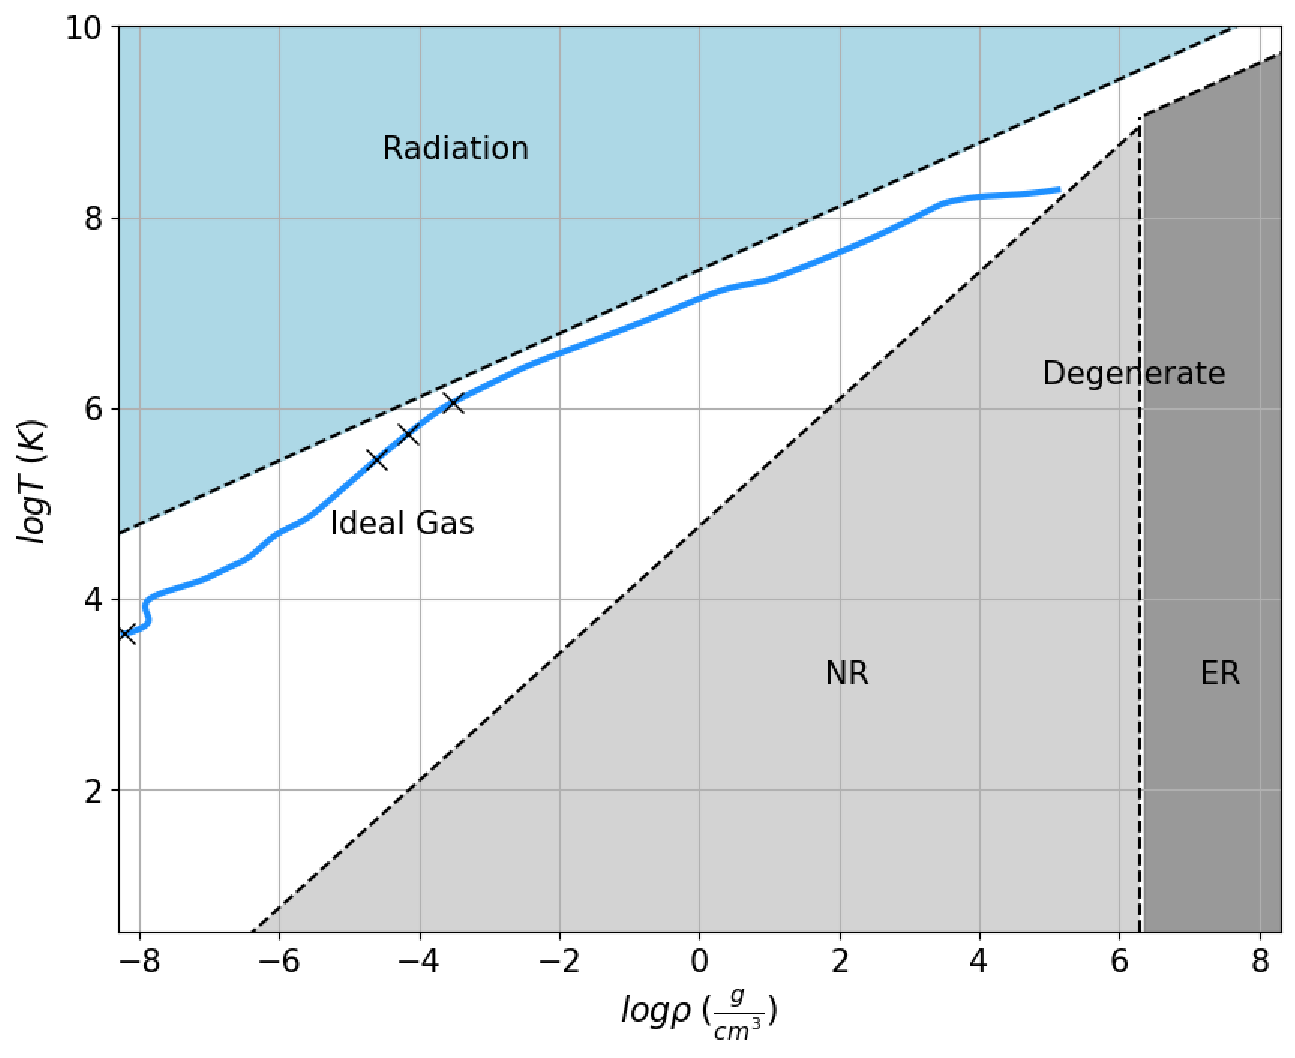
\includegraphics[width=0.9\textwidth]{Thesis/graphs/eos.pdf}
    \caption{ The radial structure of the outer star at the moment of \ac{rlof} in the  temperature-density plane. I calculate the stellar profile using MESA \citep{paxton2010modules,paxton2013modules,paxton2015modules,paxton2019modules}.}
    \label{fig:eos}
\end{figure}
At the moment of \ac{rlof} the pressure within the envelope is dominated by the ideal gas component, see \cref{fig:eos}. Thus I can indeed neglect the radiative part of \cref{eq:pressure}. Using
\begin{equation}\label{eq:pressure_ideal_gass}
    P(r) =  \frac{\mathcal{R}}{\mu(r)} \rho(r) T(r)
\end{equation}
each particle is allocated a unique specific internal energy based on the temperature and mean molecular mass profiles:
\begin{equation}\label{eq:internal_energy}
    u(r) = \frac{3}{2} \frac{k_B T(r)}{\mu(r)},
\end{equation}
where $k_B$ is the Stefan-Boltzmann constant, $T(r)$ and $\mu(r)$ the temperature and mean molecular mass profiles, respectively.

The particles at this point are kinematically cold meaning that their specific kinetic energies are zero and only their internal and potential energies contribute to the total energy of the gas. This is illustrated in \cref{fig:kinetic_internal_energies}, where I present 2D maps of the kinetic and internal particle energies, respectively.
\begin{figure}[H]
    \centering
    \begin{subfigure}{.5\textwidth}
    \centering
    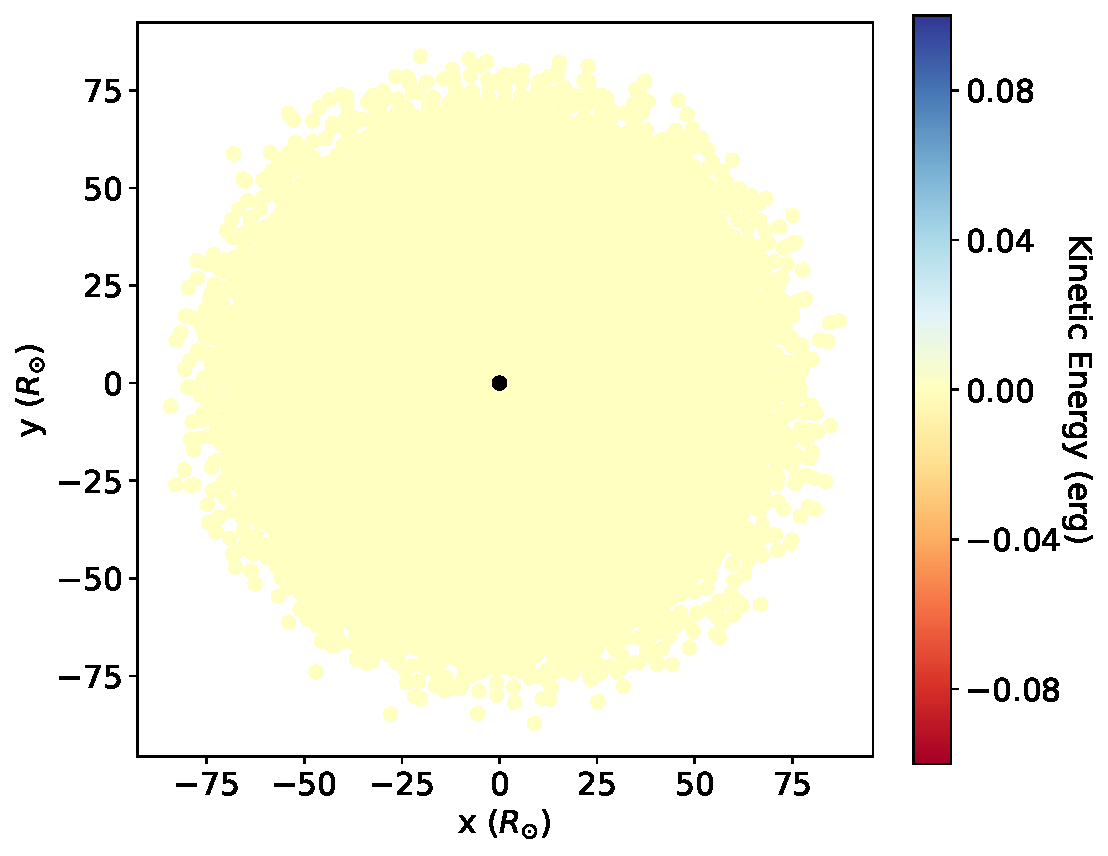
\includegraphics[width=0.9\textwidth]{Thesis/graphs/tertiary_kin_energy_before_relaxation.pdf}
    \label{fig:mass_loss}
    \end{subfigure}%
    \begin{subfigure}{.5\textwidth}
    \centering
    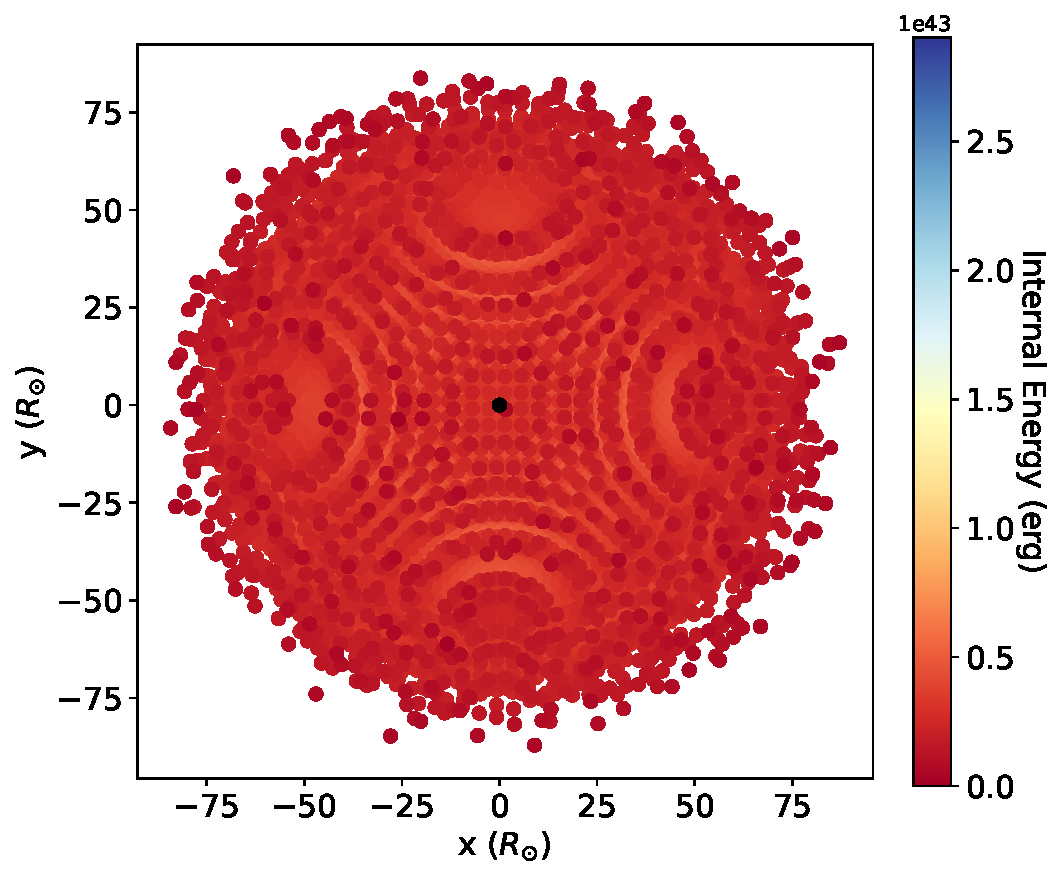
\includegraphics[width=0.9\textwidth]{Thesis/graphs/tertiary_internal_energy_before_relaxation.pdf}
    \label{fig:radius_profile}
    \end{subfigure}
    \caption{ Kinetic and internal energies of the gas particles after converting the 1D stellar evolution model to a 3D gas particle distribution. The black point corresponds to the core particle which is a pure gravitational point mass with no pressure or internal energy.}
    \label{fig:kinetic_internal_energies}
\end{figure}
Another important parameter of the gas is its specific entropy. It is often mathematically simpler, although not formally necessary, to define an entropic variable $A$. The entropic variable $A$ is closely linked (but not identical) to the specific entropy and it is defined as
\begin{equation}\label{eq:entropic_variable}
    A(r) \equiv \frac{P(r)}{\rho(r)^{\gamma_{ad}}}
\end{equation}
where $\gamma_{ad}$ is the adiabatic index, and $P(r)$ and $\rho(r)$ the pressure and density profiles, respectively. 

The evaluation of the original entropic profile $A(r)$ of the stellar envelope is not trivial and one needs to consider the relevant pressure sources, see \cref{eq:pressure}. In a radiation-dominated gas, $\gamma_{ad} = 4/3$ is a more suitable adiabatic index (this is in general true when extremely relativistic particles dominate), while for a mixture of gas and radiation, $4/3 \leq \gamma \leq 5/3$. However, at the moment of \ac{rlof}, see \cref{fig:eos}, ideal gas is the dominant radiation pressure source, thus considering \cref{eq:internal_energy} and \cref{eq:entropic_variable}, I calculate the entropic profile $A(r)$ with $\gamma = 5/3$, such as:
\begin{equation}\label{eq:entropic_variable_2}
    A(r) = \frac{2}{3} u(r) \rho(r)^{-2/3}.
\end{equation}

\subsection{Stellar envelope: Radiative case}\label{sub:envelope_rad}

In the previous subsections I showed how I model $\xi$ Tau's outer component. The presented method works pretty well due to the fact that the envelope is convective at the onset of \ac{rlof}. I tested the scenario of \ac{rlof} occurring at different phases of the evolution, when the envelope is radiative, and for different initial stellar masses. Hence, I present the additional parameters that need to be considered in the case of a radiative envelope. These key points can be incredibly valuable and time-saving for future work using the same method.

Low-mass, thus cold, stars have convective envelopes during their evolution, while massive stars with M$>16$M$_{\odot}$ remain with a radiative envelope pretty much until the end of their lives. Intermediate- and high-mass stars' envelopes (M  $<16$M$_{\odot}$) can be either convective or radiative depending on the evolutionary phase in which \ac{rlof} occurs, see \cref{sec:single_star_evolution}. 
\begin{figure}[H]
    \centering
    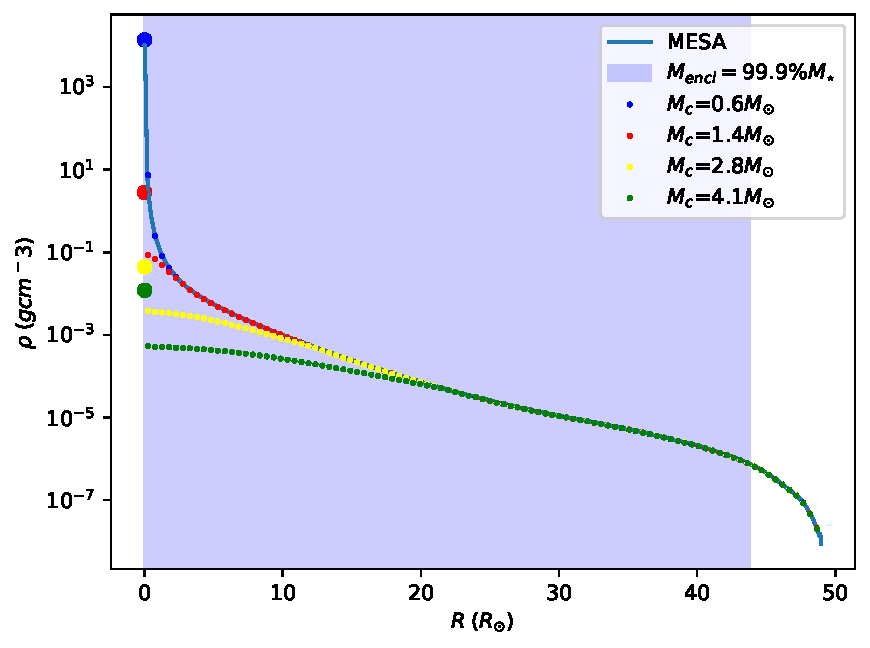
\includegraphics[width=0.9\textwidth]{Thesis/graphs/density_profile_radiative_envelope.pdf}
    \caption{Radial density profile of the  $\xi$ Tau outer component at $t=78.3$ Myr (blue line), when the star is in its helium-burning phase and has a fully radiative envelope. MESA's 1D density profile of the tertiary is shown by the solid blue line. The shaded region represents 99.9\% of the star's enclosed mass. The dotted lines depict \ac{sph} models with varied core masses, M$_{core}$, which correspond to fractions of 0.1, 0.255, 0.5, and 0.75 of the overall mass of 5.5 M$_{\odot}$, while the larger points correspond to core particle densities, respectively.}
    \label{fig:density_profile_radiative}
\end{figure}
The density within a convective envelope falls of with pressure $\rho \propto P^{1/\gamma_{ad}}$, see \cref{eq:adiabatic_eos}. If the envelope is stable against convection, the density gradient must vary more steeply with pressure than for an adiabatic change by definition. This means that radiative envelopes are less dense in the outer layers and more centrally concentrated than convective envelopes \cite{pols2011stellar}. This is reflected in \cref{fig:density_profile_radiative}, where I plot the tertiary's radial density profile at $t=78.3$ Myr, when the star is in its helium-burning phase and has a fully radiative envelope, see \cref{fig:kippen_plot}.

Modeling the radiative envelope case is more challenging. From the computational point of view, the problem branches in to two sub-problems. First, a comparison between \cref{fig:stellar_density_ROLF} and \cref{{fig:density_profile_radiative}} immediately reveals the difference in scales. More specifically, in the radiative case someone needs to resolve 6-8 orders of magnitude in density. In \cref{fig:density_profile_radiative}, I use $N=10^6$ particles and still the outer layers of the star are not very well resolved. This is a direct consequence of the density's profile high steepness and the use of equal mass particles. In general, the use of equal mass particles provides good resolution in high-density regions, however, only poorly resolves low-density regions. Second, using $N$ of 6 orders of magnitude, will result in extremely long computational time, as the CPU simulation time is not linear function of $N$, but rather the CPU time increases with the number of \ac{sph} particles as $NlogN$.

The problematic steepness of the density profile becomes more severe for high-mass stars. Additionally, as stellar mass grows so does the importance of radiation pressure. From a physics standpoint, someone must estimate the importance of radiation in order to accurately define the thermodynamic properties of the gas using \cref{eq:pressure}, \cref{eq:entropic_variable} and a proper adiabatic index, $\gamma_{ad}$.

In conclusion, the method is preferable for modeling low- and intermediate-mass stars with convective envelopes. For high-mass stars, even if the thermodynamic properties of the gas are defined properly, the intrinsic steepness of the density profile will remain.  Hence, a very high number of \ac{sph} particles are needed to resolve the stellar envelope, which result in very long computational times. 




\begin{comment}
    This parameter will be important in order to adjust correctly thermodynamic properties of the gas inside the softened zone.
\end{comment}

\section{Bringing the 3D hydrodynamical model in hydrostatic equilibrium}

Up to this point, I have specified most of the 3D hydrodynamical model's parameters, which would be simulation's starting point. However, an extremely unstable model would result from entering these values into GADGET-2, where the gas particles would quickly reach arbitrary high velocities and escape.

There are two causes for this behavior, and as a result, there are two additional phases I must complete before I can produce a smooth and stable 3D hydrodynamical model. The first is related to the softening length of the core particle, while the second is related to the initial gas particle accelerations as being calculated by GADGET-2 via gravitational forces and pressure gradients. In the next two subsection I will expand upon how I tackle these challenges. 

Furthermore, I consider an adiabatic \ac{eos}, see \cref{eq:adiabatic_eos}, with $\gamma_{ad} = 5/3$, in GADGET-2 for the gas. Hence, the simulaitons include adiabatic cooling and heating due to expansion and contraction of the gas, respectively. This decision is predicated on the fact that the simulation run time is more than two orders of magnitude shorter than the $t_{th}$ of the tertiary, see \cref{tab:tertiary_timescale_ROLF}. If $t_{th}$ was significantly shorter than the current value, an isothermal \ac{eos} may be a better choice. In order to test this assumption, I run one simulation using an isothermal \ac{eos}. As expected, the model proved extremely unstable with the envelope escaping freely since it is not affected by adiabatic cooling.

\subsection{Core particle softening length}

Since I consider the core particle to be a pure gravitational point mass with no pressure or internal energy, I need to avoid the star from collapsing on itself.
To achieve that, I use Plummer softening, $\epsilon$, to soften the core particle. Similar with GADGET-2, I adopt the conventional cubic spline of \cite{monaghan1985refined}, which drops to zero smoothly at $2.8 \epsilon$, see Eq. \eqref{eq:spline_kernel}. The density and internal energy inside the softened zone are adjusted so that pressure equilibrium is maintained while the original entropic variable $A$ is preserved, see \cref{sub:envelope_conv}. 

The motivation behind that is known as entropy sorting and it is derived by simulations of stellar collisions \citep{lombardi1995collisions,lombardi2003modelling,lombardi2006stellar,gaburov2008mixing,gaburov2010onset}, where both the entropic variable and the specific entropy are preserved in the absence of shocks and increase in their presence. To put it simply, the fluid with the highest entropy should be on top of the fluid with the lowest entropy in order to establish hydrodynamic stability. 

Defining a good $\epsilon$ has been proved a major challenge. I run a series of short convergence tests varying the number of particles $N$ and the core particle mass, $M_c$. The tests proved that the choice of the softening length, $\epsilon$, depends weakly on $N$, and strongly on $M_c$, which is related to the tertiary's mass at the moment of \ac{rlof}, see \cref{tab:core_masses_ROLF}. I demand two criteria to be fulfilled, at the same time, for selecting a good softening length:
\begin{itemize}
    \item The selected $M_c$, and hence the respective softening length, should result to a 3D density profile which agrees with MESA's 1D density profile.
    \item For a given $M_c$, and hence the respective softening length, the star should not collapse on itself at the beginning of the simulation.
\end{itemize}
The first criterion allowed me constraint my parameters' search, see \cref{fig:stellar_density_ROLF}. For the adopted $M_c$=0.255 M$_{ROLF}$, I present the parameters of the convergence tests
\begin{table}[H]
    \centering
    \begin{tabular}{| c | c | c |}
       M$_{core}$  & N & $\epsilon$/$R_{RLOF}$ \\
       \hline
       25.5\% M$_{RLOF}$ & $10^4$ & 0.1\\
       25.5\% M$_{RLOF}$ & $10^4$ & 0.15\\
       25.5\% M$_{RLOF}$ & $10^4$ & 0.2\\
       25.5\% M$_{RLOF}$ & $10^4$ & 0.25\\
       25.5\% M$_{RLOF}$ & $10^4$ & 0.3\\
       25.5\% M$_{RLOF}$ & $10^4$ & 0.4\\
       \hline
       25.5\% M$_{RLOF}$ & $50^4$ & 0.1\\
       25.5\% M$_{RLOF}$ & $50^4$ & 0.15\\
       25.5\% M$_{RLOF}$ & $50^4$ & 0.2\\
       25.5\% M$_{RLOF}$ & $50^4$ & 0.25\\
       25.5\% M$_{RLOF}$ & $50^4$ & 0.3\\
       25.5\% M$_{RLOF}$ & $50^4$ & 0.4\\
    \end{tabular}
    \caption{ Parameters of the convergence tests to adopt a softening length, $\epsilon$, for the tertiary at the beginning of \ac{rlof}.}
\label{tab:smoothing_length_exploration}
\end{table}
The tests proved that an $\epsilon \in [0.14-0.2] R_{RLOF}$ can fairly satisfy both criteria. I adopt $\epsilon = 0.16 R_{RLOF}$ which provide very good results.

At this point, it is interesting to mention that an $\epsilon \in [0.14-0.2] R_{RLOF}$ seems to satisfy the first criterion for any $0.2M_{RLOF} < M_c \leq 0.5M_{RLOF}$, given a convective envelope. After running more than 20 convergence tests varying all parameters listed in \cref{tab:smoothing_length_exploration}, I establish a rule of thumb, where $\epsilon \in [0.14-0.2] R_{RLOF}$ provides a stable hydrodynamical model given a convective envelope. This might be a good starting point for future efforts to simulate hydrodynamically stable giants with a pure gravitational point mass representing the inner high density zone.

\subsection{Relaxation}

The initial particle accelerations as determined by the \ac{sph} algorithm are not zero, despite the initial particle distribution being as smooth as feasible. This is most likely caused by a combination of factors:
\begin{enumerate}
    \item MESA and GADGET-2 adopt a different \ac{eos}. Specifically, a variable and a fixed adiabatic index $\gamma_{ad}$, respectively.
    \item Numerical artifacts of using a (scaled) regular grid in low-density region, see \cref{fig:stellar_density_ROLF}.
    \item Implications of the \ac{sph} code's implementation of gravitational softening.
    \item Treatment of particles at the surface, with anisotropic neighbour distributions.
\end{enumerate}
Neglecting these non-zero particle accelerations will produce erroneous turbulent velocities. The internal energy of the particles will subsequently grow as a result of viscous damping. Therefore, to prevent artificial heating for my model, relaxation is necessary.

Relaxation is a process that involves allowing a system to evolve over time towards its equilibrium state through the dissipation of energy. The \ac{sph} algorithm iteratively adjusts the positions $x_i$ and velocities $v_i$ of the particles based on their interactions with neighboring particles, while during the process the center-of-mass position, $R_{cm}$, and velocity $V_{cm}$ are preserved. In simple words the star oscillates towards a more hydrodynamically stable state. The internal velocities are dampened by multiplying by a factor $f$ that grows adiabatically from 0 to 1:
\begin{equation}\label{eq:adjust_positions}
    x_{i,adjusted} = x_i - R_{cm} + R_{cm,initial}
\end{equation}
\begin{equation}\label{eq:adjust_velocities}
    v_{i,adjusted} = f \times (v_i - V_{cm}) + V_{cm,initial}
\end{equation} 
Furthermore, I perform relaxation in isolation meaning that during the process the 3D hydrodynamical model is not `feeling` the potential of the inner binary. It is not easy to quantify the inherent error introduced by this assumption. The gravitational force experienced by the gas particles as a result of the binary will be proportional the mass of the binary components, and inversely proportional to their distance from them. This is a detail that may be significant in the case of simulating a triple system, where the inner binary components are relatively heavier stars and the orbital period of the outer orbit relatively shorter.

Determining the relaxation's duration is not trivial. Ideally, someone would want to perform relaxation until the model reaches a state of perfect equilibrium. On one hand, this not possible and more importantly very computationally expensive. On the other hand, taking shots in the dark is not absolutely necessary. I may start by choosing a lower and upper limit that fulfil basic physical criteria.

For the lower limit, the process should simply reduce numerical noise to an acceptable level. In simple words, at the end of the process the gas particles should be `relaxed` enough that the envelope does not escape freely. For the upper limit, the process duration should be related to the dynamical timescale of the star, see \cref{eq:dynamical_timsecale} and \cref{tab:tertiary_timescale_ROLF}. This comes from the definition of the dynamical timescale, which refers to the time needed for a star to restore dynamical equilibrium after it has been disturbed. Hence, the relaxation's duration should not be significantly longer than the dynamical timescale of the star. As a result, I choose  $t_{relax} = 10 t_{dyn}$ as an upper limit and perform the process using $n_{steps} = 100$, hence each step corresponds to $dt=0.4835$ day, see \cref{tab:tertiary_timescale_ROLF}. I present 2D maps of kinetic particle energies at $t_{relax} =[2.5, 5, 7.5, 10] t_{dyn}$.
\begin{figure}[H]
    \centering
    \begin{subfigure}[b]{0.49\textwidth}
        \centering
        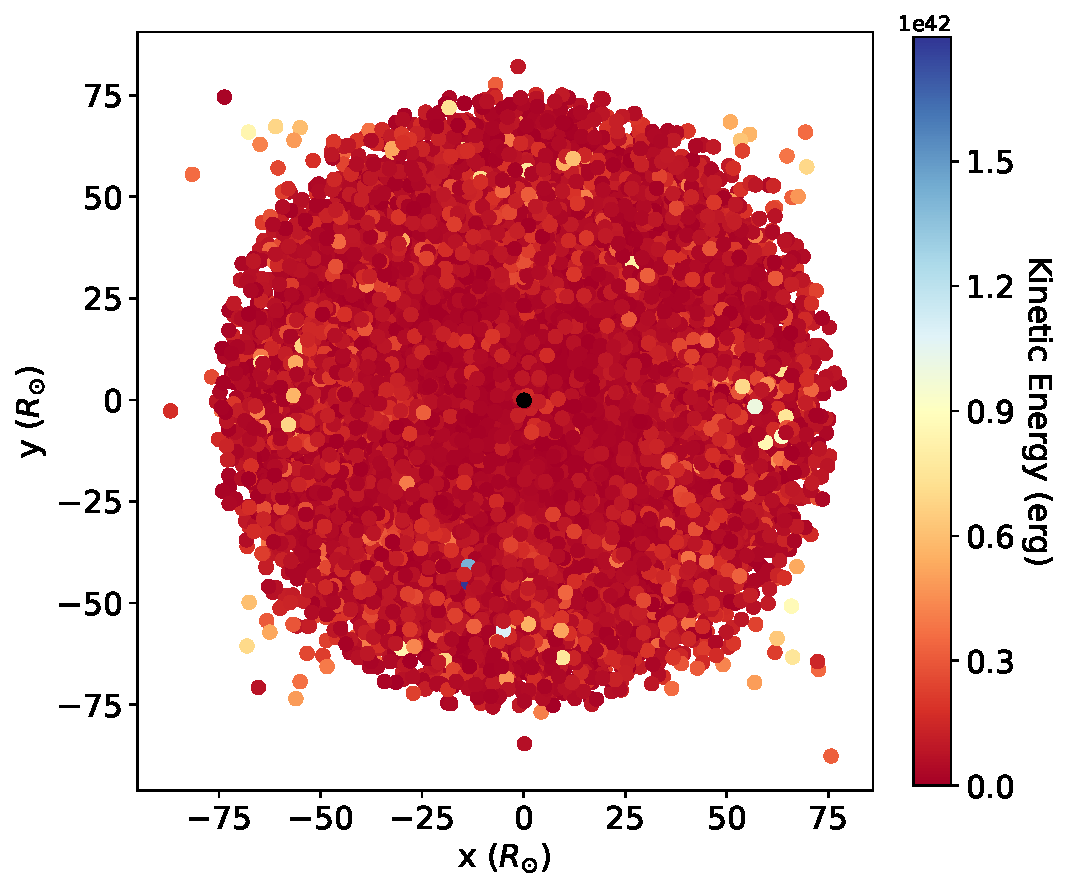
\includegraphics[width=\textwidth]{Thesis/graphs/tertiary_kin_energy_relaxed_2_5_tdyn.pdf}   
        \caption{Kinetic energies of the gas particles at  $t_{relax} = 2.5t_{dyn}$}%
    \end{subfigure}
    \hfill
    \begin{subfigure}[b]{0.49\textwidth}  
        \centering 
        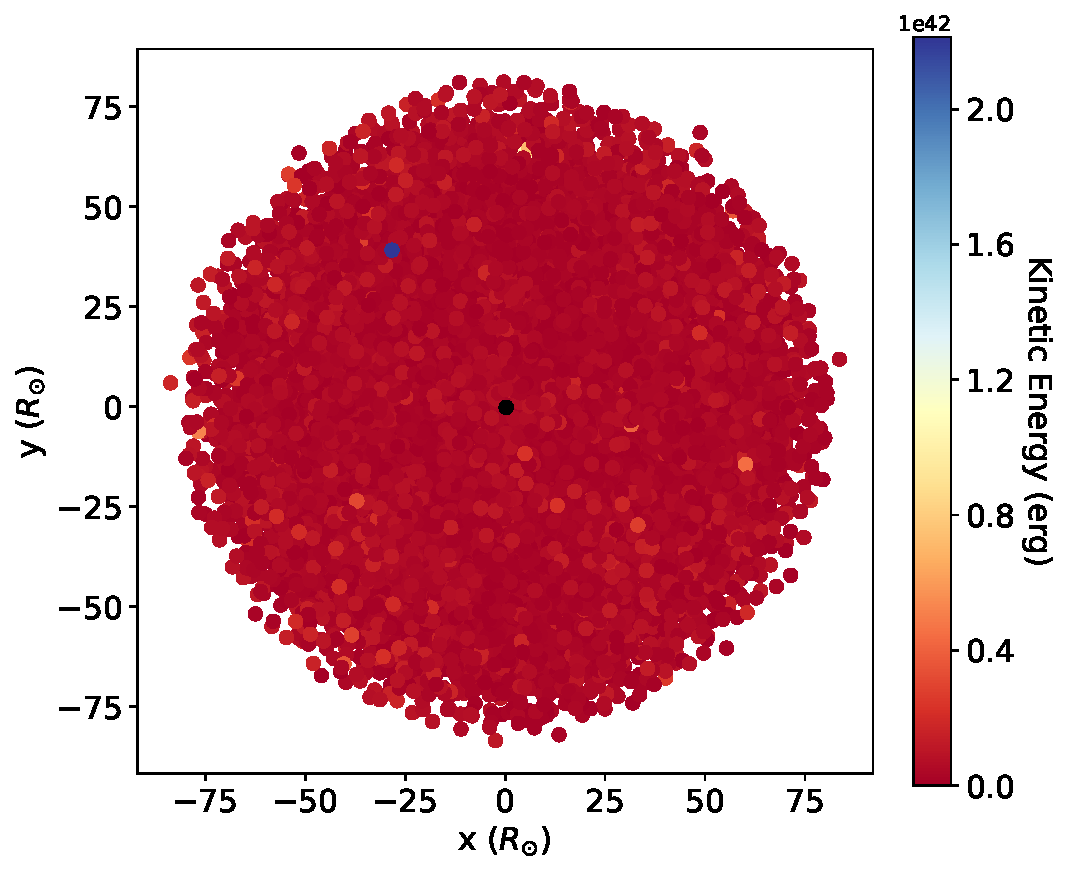
\includegraphics[width=\textwidth]{Thesis/graphs/tertiary_kin_energy_relaxed_5_tdyn.pdf}
        \caption[]%
        {{\small Kinetic energies of the gas particles at  $t_{relax} = 5t_{dyn}$}}
    \end{subfigure}
    \vskip\baselineskip
    \begin{subfigure}[b]{0.49\textwidth}  
        \centering 
        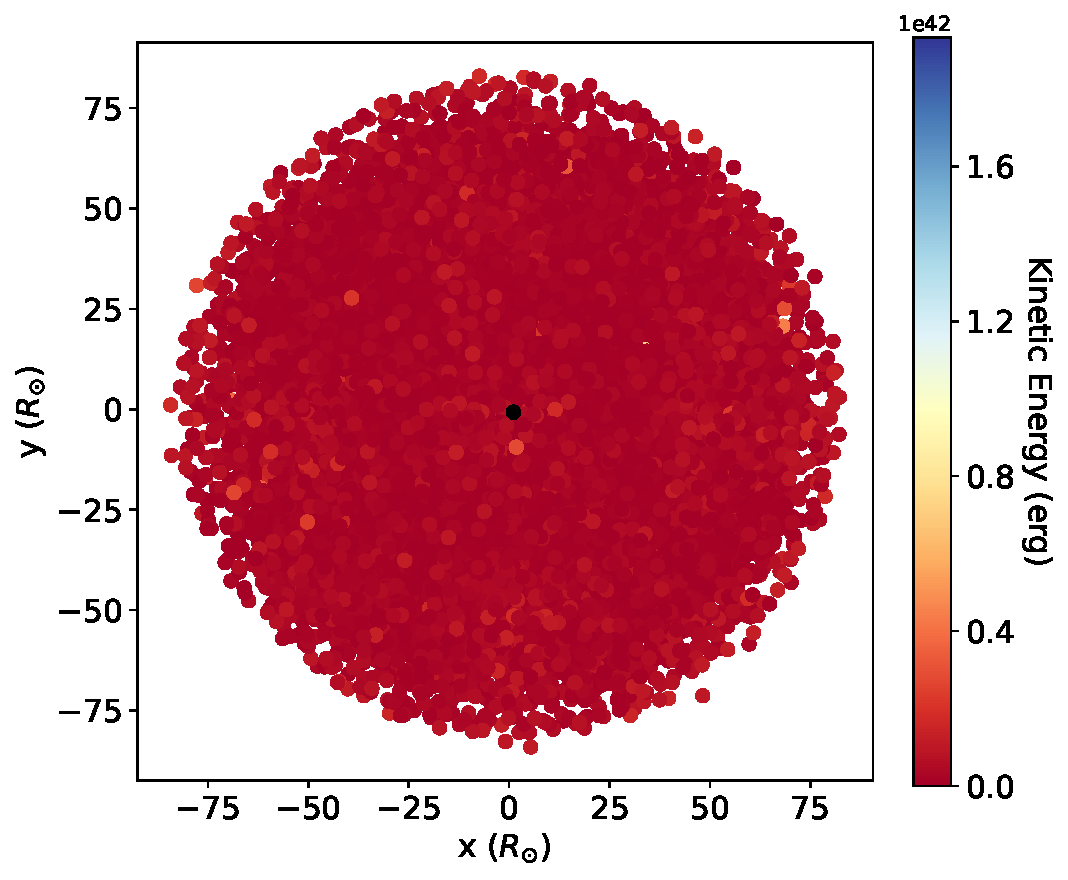
\includegraphics[width=\textwidth]{Thesis/graphs/tertiary_kin_energy_relaxed_7_5_tdyn.pdf}
        \caption[]%
        {{\small Kinetic energies of the gas particles at  $t_{relax} = 7.5t_{dyn}$}}
    \end{subfigure}
    \hfill
    \begin{subfigure}[b]{0.49\textwidth}  
        \centering 
        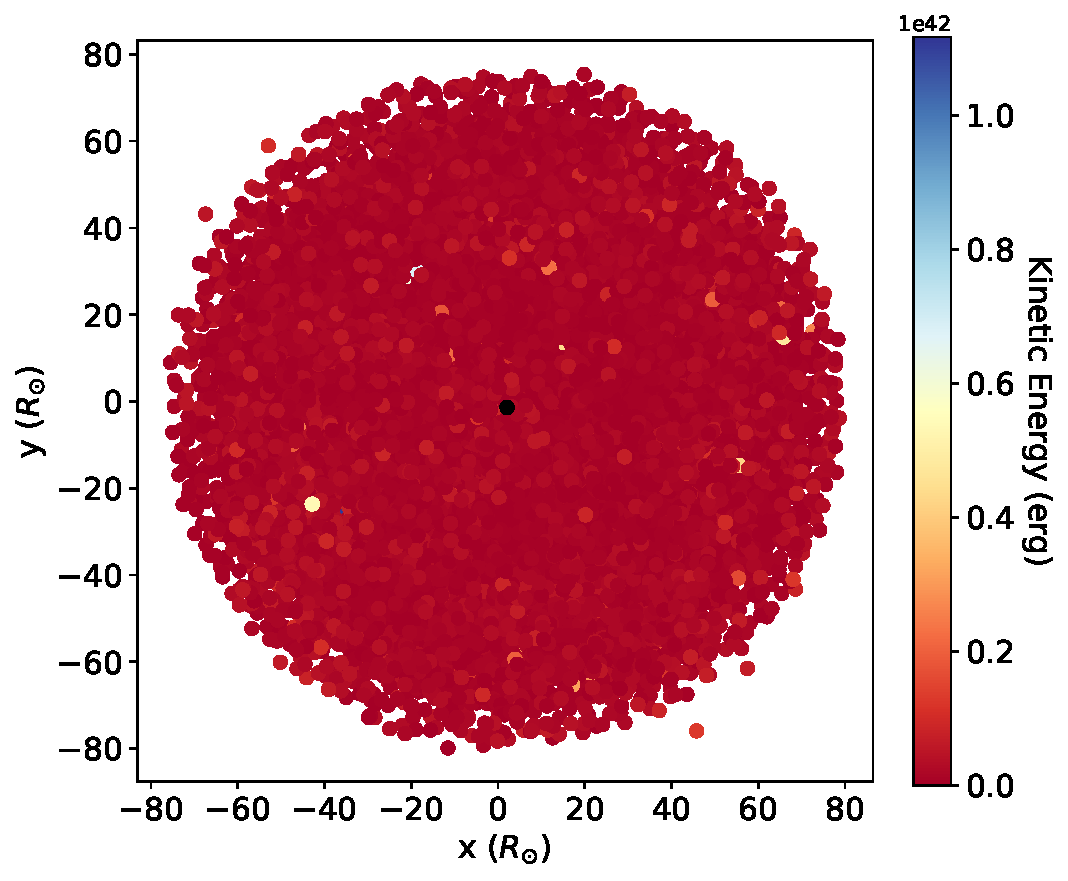
\includegraphics[width=\textwidth]{Thesis/graphs/tertiary_kin_energy_relaxed_10_tdyn.pdf}
        \caption[]%
        {{\small Kinetic energies of the gas particles at  $t_{relax} = 10t_{dyn}$}}
    \end{subfigure}
    \caption{2D maps of gas particles kinetic energies during relaxation.
    The chronological order is from left to right and from top to bottom as depicted on the respective labels. The black point corresponds to the core particle which is a pure gravitational point mass with no pressure or internal energy.}
    \label{fig:kin_energy_maps_relaxation}
\end{figure}
\cref{fig:kin_energy_maps_relaxation} shows the re-adjustment of particle positions and velocities based on \cref{eq:adjust_positions} and \cref{eq:adjust_velocities}. As the 3D hydrodynamical model becomes more spherically symmetric and the particles' kinetic energy decreases, it gradually moves towards a more hydrodynamically stable state. The latter is more apparent in \cref{fig:total_kin_energy_relaxation}, where
I present the total kinetic energy of the gas particles at $t_{relax} =[2.5, 5, 7.5, 10] t_{dyn}$.
\begin{figure}[H]
    \centering
    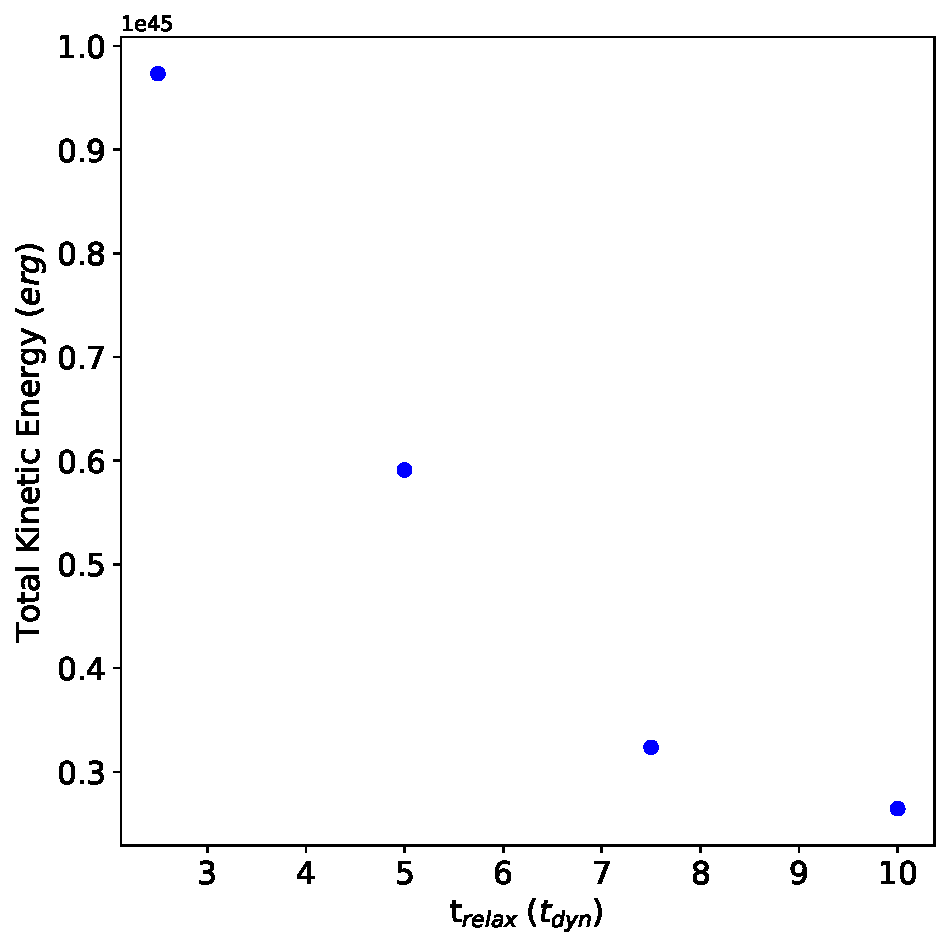
\includegraphics[width=0.9\textwidth]{Thesis/graphs/total_kientic_energy_during_relaxation.pdf}
    \caption{Evolution of the total kinetic energy of gas particles during relaxation. The blue points correspond to $t_{relax} =[2.5, 5, 7.5, 10] t_{dyn}$, respectively.}
    \label{fig:total_kin_energy_relaxation}
\end{figure}
















\section{Setting up the system}

The initial positions and velocities of the three stars are chosen such as they correspond to the orbital parameters given in \cref{tab:system_orbit_param}. The orientation of the inner orbit with respect to the outer orbit is defined by the inclination, $i$, longitude of the ascending note, $\Omega$, and argument of periastron, $\omega$ of the inner orbit relative to the outer orbit. Among these three parameters, mutual inclination is predicted to have the greatest influence on mass transfer, hence its a free parameter to be explored.  Additionally, I assume that  $\Omega=0^{\circ}$, effectively the line of nodes corresponds to the line connecting the inner binary components and $\omega= 90^{\circ}$. The effective potential of $\xi$ Tau corresponding to the initial configuration of the system is depicted in \cref{fig:triple_equop}.
\begin{figure}[H]
    \centering
    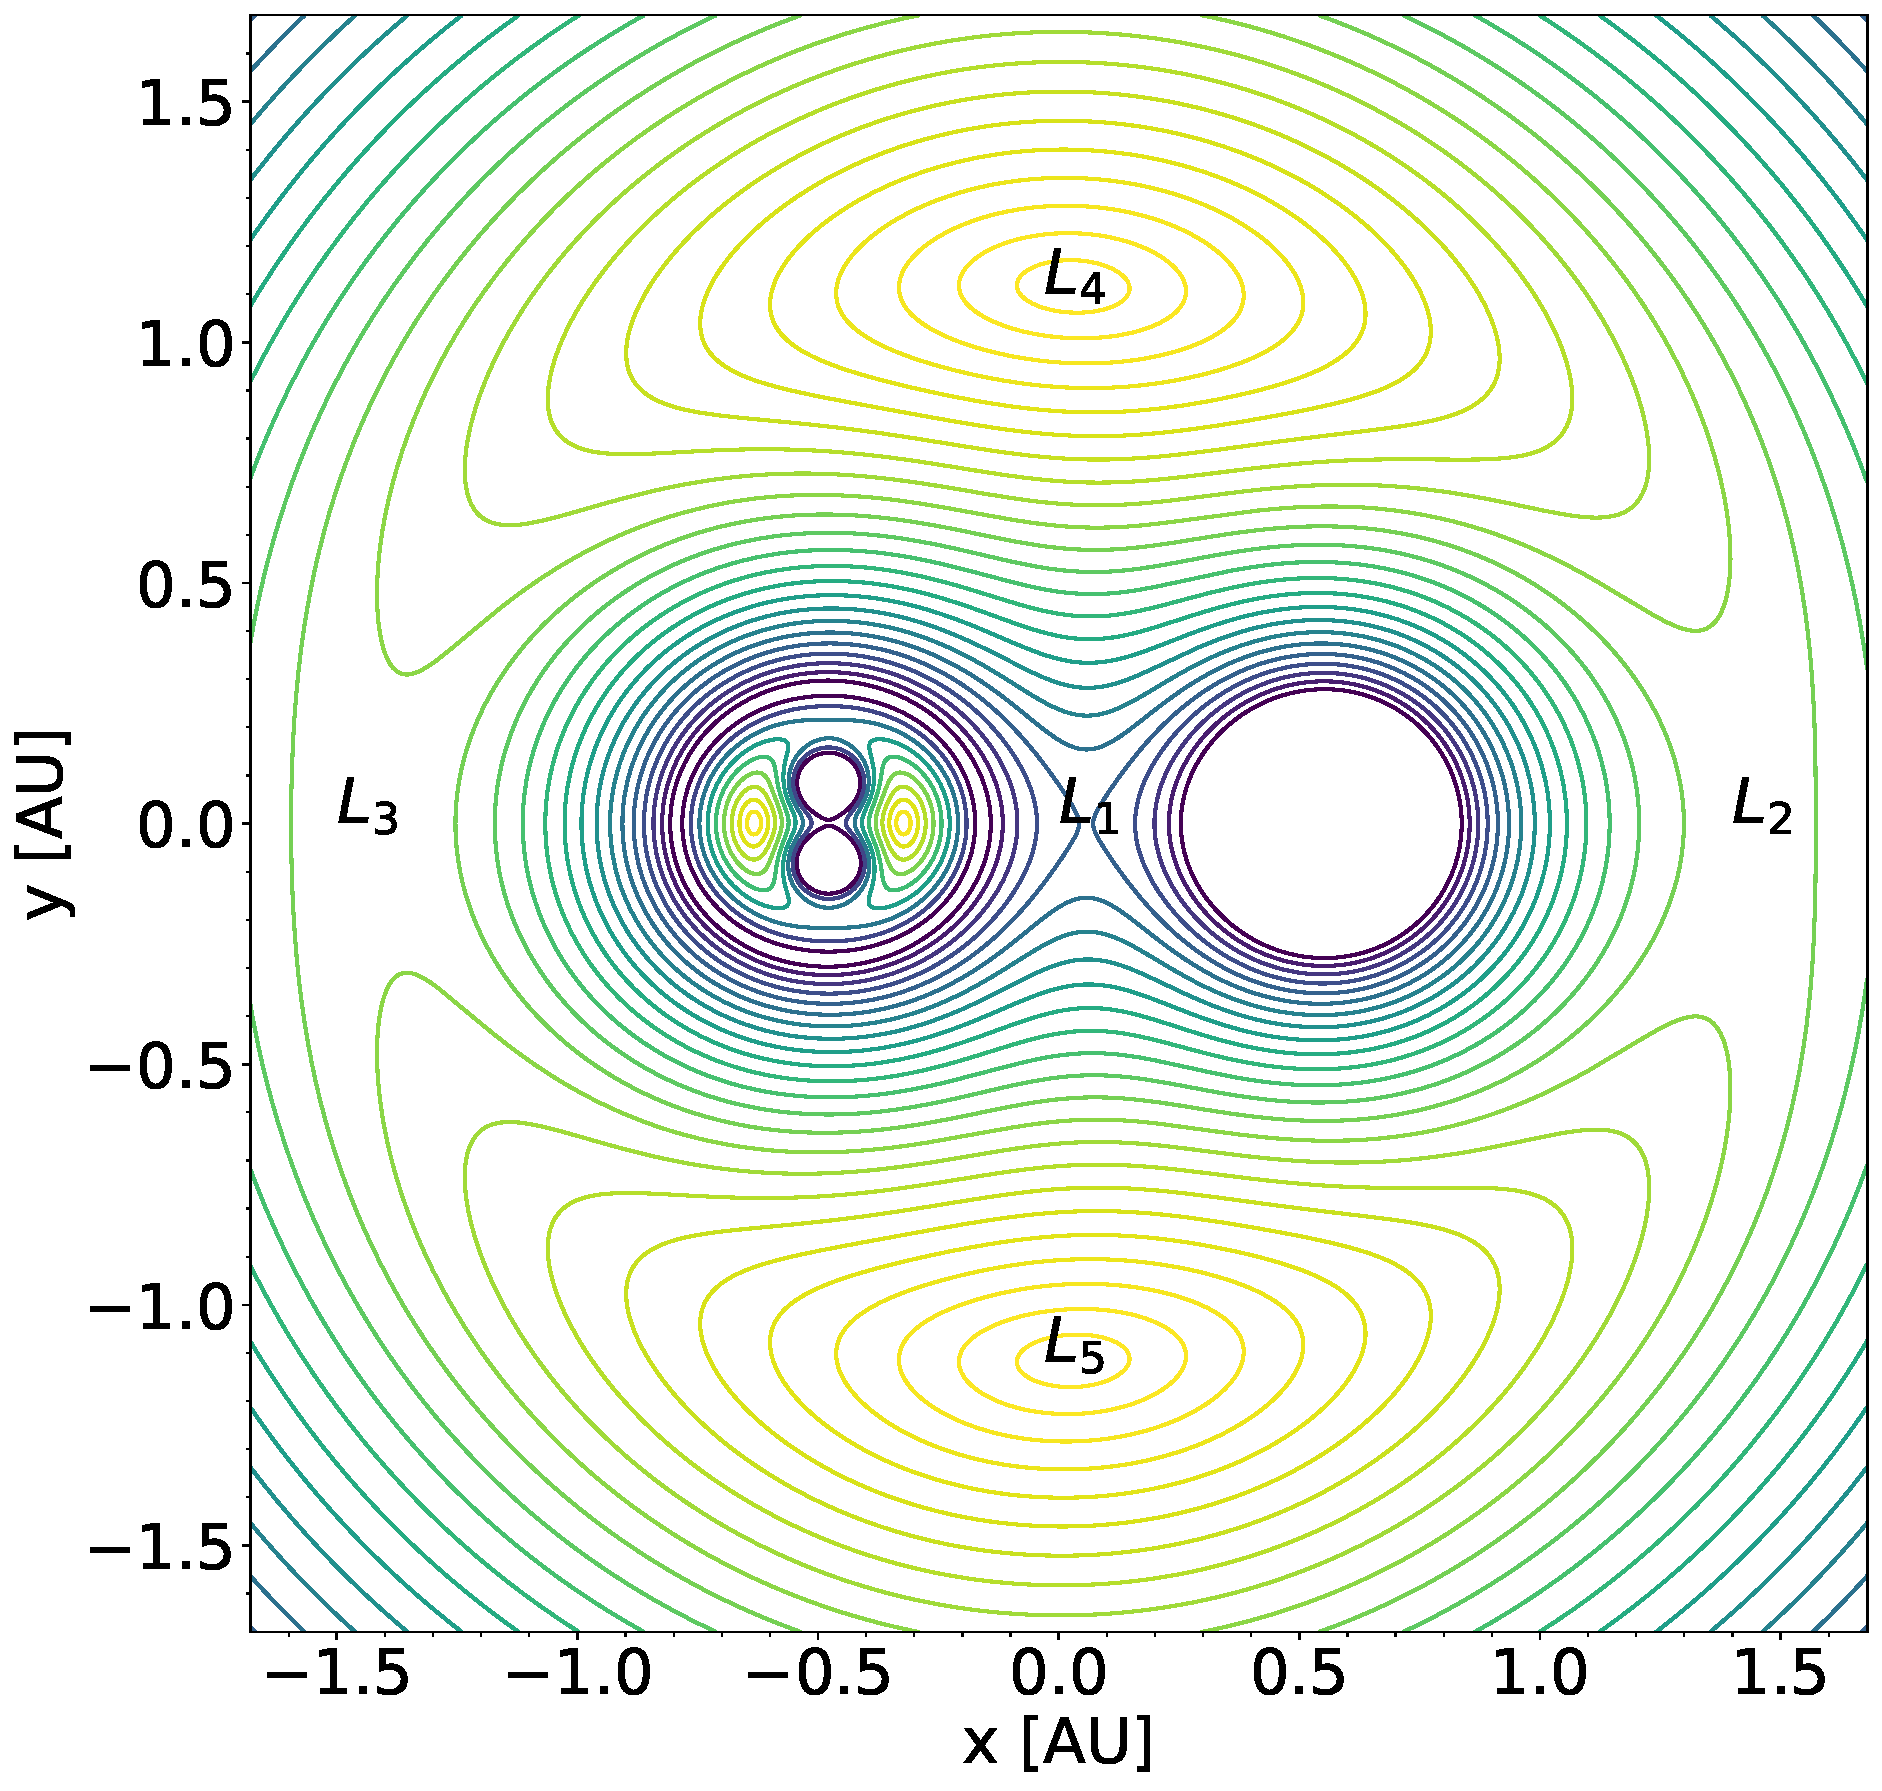
\includegraphics[width=0.9\textwidth]{Thesis/graphs/triple_equop.pdf}
    \caption{Contour plot of $\xi$ Tau's effective potential. The five Lagrangian points of the outer orbit are indicated as $L_1, L_2, L_3, L_4$ and $L_5$. I create this plot using the Hermite integrator which is part of  AMUSE \citep{hut1995building}.}
    \label{fig:triple_equop}
\end{figure}
After relaxing the 3D hydrodynamical model for $t_{relax} =10 t_{dyn}$, I have successfully created a fairly stable model, which represents the outer star. I now replace the outer star, which was a point mass until now, with the 3D hydrodynamical model. Based on the initial configuration the system is well inside the stable regime, see \cref{eq:stability_regime}, the octupole term, $\epsilon_{oct} = 0.00$, see \cref{eq:octupole_term}, thus it is not expected to be important, while the timescale of Lidov-Kozai cycles, see \cref{eq:lidov_kozai_timescale}, is $t_{koz}$ = 16.81 yr.
\section{Coupling hydrodynamics with gravity in the evolution model}

In order to encapture accurately all the details of system's evolution during mass transfer and in self consistent way, it is necessary to employ an accurate gravity solver and a method to handle the system's hydrodynamics. In general, SPH codes use low-accuracy gravity solvers and the details of the complex three-body gravitational dynamics may not be handled properly, e.g. the details of the Lidov-Kozai cycles. Hence, I employ the semi-symplectic direct N-body integrator Huayno, see \cref{sub:huayano}, to integrate equations of motion of the inner binary components, while the hydrodynamics and self-gravity of the 3D hydrodynamical model are handled by GADGET-2, see \cref{sub:gadget2}. 

In order to couple the two codes in the evolution model, I utilize the Astrophysical Multi-purpose Software Environment (AMUSE, \cite{pelupessy2013astrophysical,portegies2018astrophysical}), a comprehensive computational tool, to accurately simulate and solve for these physical processes in a self-consistent manner.  The software is written in Python and allows users to combine multiple astrophysical codes into a single simulation. 

\subsection{The bridge method}

The key feature of AMUSE is the Bridge method, first introduced by \cite{fujii2007bridge} and used to combine two different gravity solvers. The coupled integrator divides the Hamiltonian of the combined solution and iteratively integrates it with robust numerical integration techniques. As a result, the method can be implemented in general when the dynamics of a system can be divided into multiple regimes \citep{zwart2013multi}. In this section, I focus on coupling gravity and hydrodynamics which is the focus of this work.

\cite{saitoh2010fast} showed that the dynamical equations for SPH evolution can be derived from a Hamiltonian formalism, hence the Bridge formalism is applicable to a separation of purely gravitational and SPH particles. In my case, GADGET-2 (see \cref{sub:gadget2}) handles the self-gravity and hydrodynamics of the gas, while Huayano (see \cref{sub:huayano}) the gravitational dynamics of the inner binary. Using the Bridge method I achieve a second-order coupling between gravitational dynamics and hydrodynamics. As a result, the hydrodynamical solver is affected by the gravitational potential of its own particles as well as the gravitational potential of the inner binary. Furthermore, the hydrodynamics, namely gas drag, impacts the orbits of the two inner stars.
\begin{figure}[H]
    \centering
    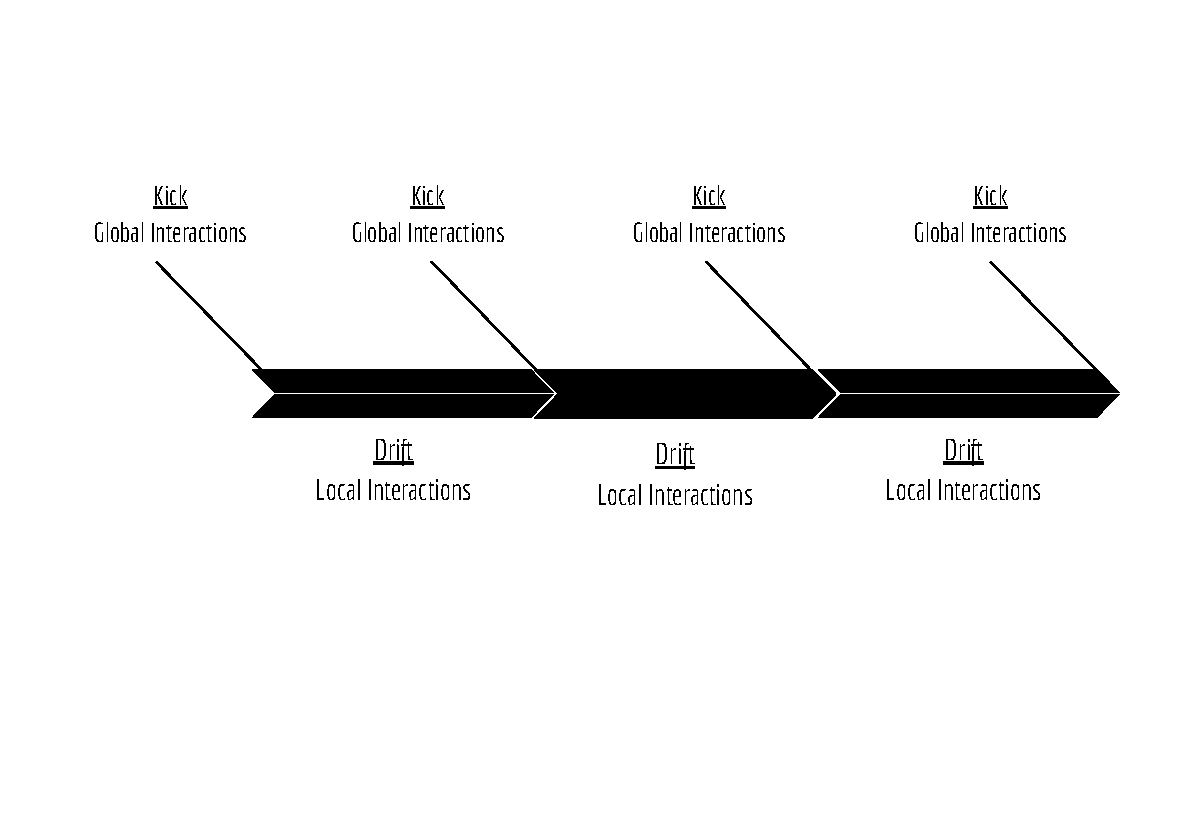
\includegraphics[width=0.9\textwidth]{Thesis/figures/kick_drift_kick.pdf}
    \caption{Schematic kick–drift–kick procedure.}
    \label{fig:kick_drift_kick}
\end{figure}
The evolution via the Bridge method can be implemented as a kick–drift–kick scheme, as illustrated in \cref{fig:kick_drift_kick}. More specifically:
\begin{enumerate}
    \item Kick (Inner Binary, Huayano): Initially, Huayano is used to calculate the gravitational forces operating on the inner binary. These forces "kick" the point masses, causing them to change velocity.
    \item Drift (Inner Binary, Huayano): With the revised velocities of the point masses, Huayano is used to evolve their positions forward in time, assuming a constant velocity over a short time period.
    \item Kick (Tertiary, GADGET-2): At this point, Bridge is used to transmit the modified positions and velocities of the point masses from Huayano to GADGET-2. The latter utilizes these positions to determine the gravitational forces exerted by the point masses on the 3D hydrodynamical model. These forces "kick" the SPH particles and the core particle, causing their velocities to change.
    \item Drift (Tertiary, GADGET-2): Now, using the updated velocities of the 3D hydrodynamical model, GADGET-2 evolves the particles positions forward in time allowing for fluid flow and interactions based on the combined effects of gravity and hydrodynamics.
    \item Kick (again) (Inner Binary, Huayano): Once again, Bridge is used, to transport the new positions and velocities of the 3D hydrodynamical model from GADGET-2 back to Huayano. Huayano recalculates the gravitational forces acting on the point masses by the 3D hydrodynamical model. These forces "kick" the point masses once more, causing their velocities to change.
    \item Drift (again) (Inner Binary, Huayano): Finally, with the updated velocities of the point masses, Huayano is used to evolve their positions forward in time again, assuming a constant velocity over a short time period.
\end{enumerate}

Each code operates on their own internal time steps, while the Bridge time step defines the time interval at which the codes interact with each other. Hence, its an important parameter to accurately model the coupling between hydrodynamics and gravity. Nevertheless, a time step, $t_{bridge}$, which is about a fraction of $1/64$ the inner binary orbital period, see \cref{tab:system_orbit_param}, provides converged solutions. 




\section{Codes' set up}

At this point, it is clear that I took many consecutive steps to model mass transfer in triple systems with a Roche-lobe filling outer star. A schematic representation of the entire process is provided in \cref{fig:schematic_method}
\begin{figure}[H]
    \centering
    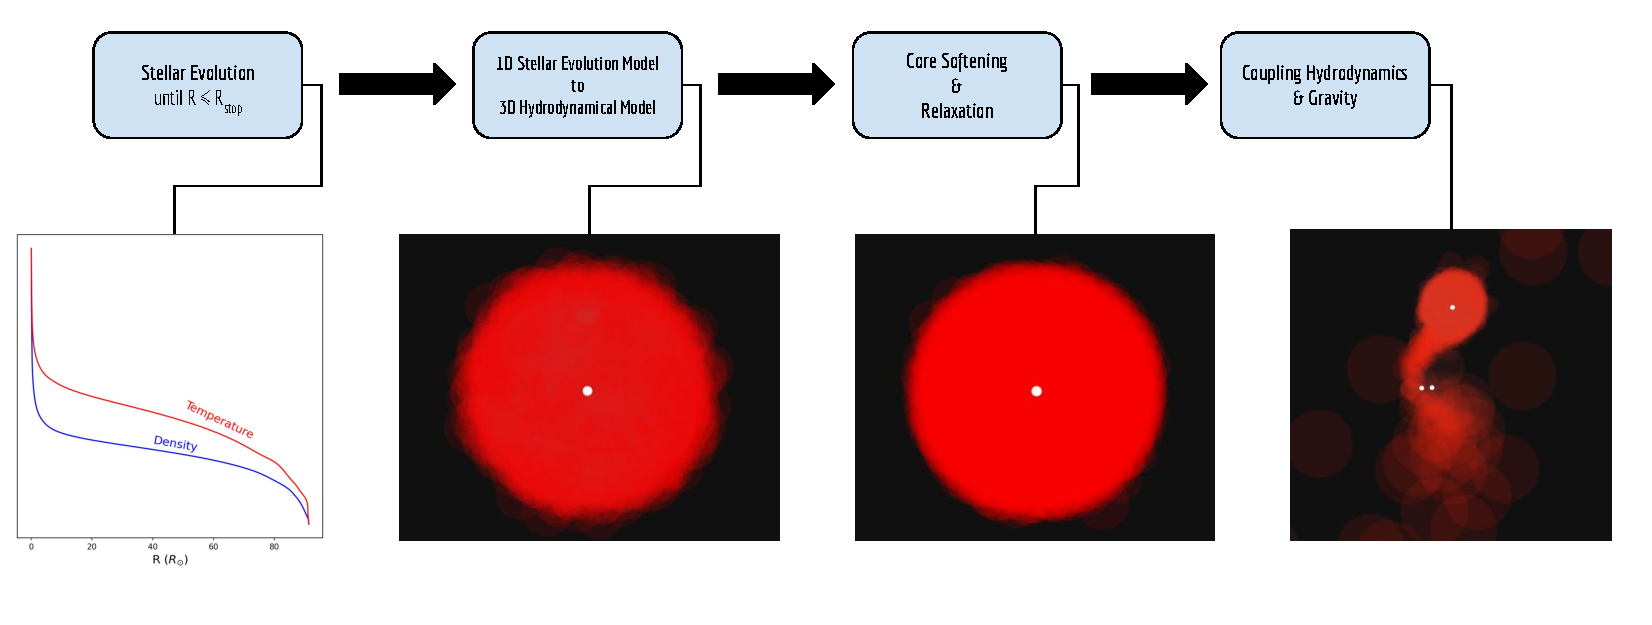
\includegraphics[width=\textwidth]{Thesis/figures/method_schematic.pdf}
    \caption{Schematic representation of the steps taken to simulate mass transfer in the triple system with a Roche-lobe filling outer star. The white points are the purely gravitational particles representing the core and the inner binary components. The red points are the \ac{sph} particles representing the gas having an adaptive smoothing length.}
    \label{fig:schematic_method}
\end{figure}
In each step, I explored the importance of different parameters and made assumptions based on relative physics to better simulate the system's behavior. The outcome of a simulation is, of course, dependent on the simulation's setup; Furthermore, knowing the setup parameters is important for the reproducibility of the results. Hence, I summarize the codes' settings used for the final simulations for the reader.
\begin{table}[H]
    \centering
    \begin{tabular}{ |p{6.5cm}||p{6.5cm}|  }
     \hline
     \multicolumn{2}{|c|}{Code Settings} \\
     \hline
     MESA & GADGET-2 \\
     \hline
     Initial Masses = [3.2, 3.1. 5.5] M$_{\odot}$& $N_{particles}=50^4$ \\
     Solar metallicity& Self-gravity: True\\
     No winds& Adaptive smoothing length: True\\
     No overshooting& Softening = smoothing length\\
     No star rotation & Adiabatic \ac{eos}  \\
     Convection-occurrence (Schwarzwild) & Time step = $1/64 \times P_{in}$ \\
     Evolve until $\geq 1.1 \times R_{RLOF}$ & Artificial viscosity: $\alpha=0.5, \beta=1.0, \eta=0.1$ \\
     \hline
    \end{tabular}
        \centering
    \begin{tabular}{ |p{6.5cm}||p{6.5cm}|  }
     \hline
     \multicolumn{2}{|c|}{Code Settings} \\
     \hline
     Huayno & AMUSE \\
     \hline
     No softening length & Gravity-Hydrodynamics (2nd-order-coupling)\\
     Default time step ($<< 1/64 \times P_{in}$) &  Bridge time step = $1/64 \times P_{in}$\\
     \hline
    \end{tabular}
    \caption{ Various important settings and flags used for the different codes and AMUSE}
\label{tab:codes_settings}
\end{table}

\section{Simulations}\label{simulations}

Mass transfer in hierarchical triple
systems and more specifically, the case of \ac{rlof} by the outer star is expected to be considerably different than mass transfer in an ordinary binary system. One reason is that the mass cannot simply be accreted by the inner
objects, but may be expelled via a slingshot effect due to the inner binary rotation. During mass transfer, the inner binary evolves as well, and both stars interact with the gas provided by the outer star and may accrete part of it. The non-accreted material may form a circumbinary disk or being expelled from the system, carrying away angular momentum, see \cref{sub:orbit_evol_mass_loss}. Simultaneously, orbital angular momentum exchange may influence the eccentricity of the inner orbit through the Lidov-Kozai cycles, see \cref{sub:lidov_kozai}. As a result, the semi-major axes ratio of the two orbits is expected to change, potentially making the system unstable, see \cref{sub:stability_triples}, increasing close encounters and even result to stellar mergers \citep{antonini2017binary,silsbee2017lidov,vigna2021massive}.

I perform in total four simulations. In order to include accretion, I use sink particles which comove with the point masses representing the inner binary stars. Each sink has a characteristic sink radius, which defines the size of the accretion region around the position of each star. If a \ac{sph} particle finds its position inside this sink radius, the particle is accreted by the sink. Hence, the \ac{sph} particle's mass and momentum are added to the sink particle, which updates the mass and velocity of the star in the computational domain.

The simulations are divided into two groups based on the sink particles' accretion radii, see \cref{tab:simulations_settings}. In the first case, the accretion radii are four times larger than the physical stellar radii. The stellar radii are calculated by MESA as each star in the system evolves until the tertiary fill its Roche lobe, see \cref{sec:stellar_evolution}. These accretion radii are slightly smaller than the Roche lobe radii of the inner binary components as they defined by the initial configuration, see inner Roche lobes in \cref{fig:triple_equop}. Here, I approximate the case of maximum accretion. In the second case, the accretion radii correspond to the physical radii of the binary components effectively representing the case of minimum accretion.

%Finally, I perform one more simulation, number 5 in \cref{tab:simulations_settings}, which effectively corresponds to a retrograde rotation of the inner orbit with respect to the outer orbit.

\begin{table}[H]
    \centering
    \begin{tabular}{| c | c | c |}
     \hline
     &Mutual Inclination, $i_{mut}$ & Accretion radius \\
    \hline
     1&$0^{\circ}$ & $R_{sink} = 4R_{\star}$\\
     2&$20^{\circ}$ & $R_{sink} = 4R_{\star}$ \\
     3&$69^{\circ}$ & $R_{sink} = 4R_{\star}$ \\
     \hline
     4&$0^{\circ}$ & $R_{sink} = R_{\star}$ \\
     %5&$180^{\circ}$ & $R_{sink} = R_{\star}$ \\
     \hline
    \end{tabular}
    \caption{ Varying parameters of the four simulations performed.}
\label{tab:simulations_settings}
\end{table}
In all models, I start the coupled gravity-hydrodynamics simulations, when the radius of the star exceeds its Roche lobe, $R_{\star} = 1.1 \times R_L$, see \cref{eq:roche_lobe}, effectively increasing the average mass-loss rate, see \cref{eq:mass_loss_rate_anal}, of the tertiary. On the one hand, all consecutive rates of change of orbital parameters are overestimated. On the other hand, I better resolve the process of \ac{rlof}. Thus, the rates of change presented in the next chapter, should be interpreted qualitatively, but their between relations can be reliably examined.

The simulations cover an eight-years period, which corresponds to $\approx 20$ orbits of the tertiary. After $t=8$ yr, the system enters the unstable regime, see \cref{eq:stability_regime}, and thus I terminate the simulations. Every $\delta t_{bridge}=0.1$ day, see \cref{tab:codes_settings}, I extract the mass, position and velocity of each particle in the computational domain. These properties are used to calculate the orbital parameters of the inner and the outer orbits. More specifically, the semi-major axis and eccentricity of the inner orbit are calculated using the relative position and velocity of the inner binary components. Furthermore, the relative position and velocity of the inner binary center of mass and the tertiary are used to determine the semi-major axis and eccentricity of the outer orbit. The calculations are based on \cref{eq:semi-major_axis} and \cref{eq:eccentricity}, where $M = M_1 + M_2$ and $M = M_1 + M_2 + M_3$ for orbital parameters of the inner and outer orbit, respectively. Finally, I calculate the outer orbit's relative inclination with respect to the inner orbit, i.e. mutual inclination, as the angle between their respective orbital angular momentum vectors.

\chapter{Simulations \& Results}\label{simulations}

\epigraph{The consciousness of AC encompassed all of what had been a Universe and brooded over what was now Chaos. Step by step, it must be done. And AC said, "LET THERE BE LIGHT!"And there was light--”}{Isaac Asimov}


Mass transfer in hierarchical triple
systems and more specifically, the case of RLOF by the outer star is expected to be considerably different than mass transfer in an ordinary binary system. One reason is that the mass cannot simply be accreted by the inner
object, but may be expelled via a slingshot effect due to the inner binary rotation. During mass transfer, the inner binary evolves as well, and both stars interact with the gas provided by the outer star and may accrete part of it. The non-accreted material may form a circumbinary disk or being expelled from the system, carrying away angular momentum, see \cref{sub:orbit_evol_mass_loss}. Simultaneously, orbital angular momentum exchange may influence the eccentricity of the inner orbit through the Lidov-Kozai cycles, see \cref{sub:lidov_kozai}. As a result, the semimajor axes ratio of the two orbits is expected to change, potentially making the system unstable, see \cref{sub:stability_triples}, increasing close encounters and even result to stellar mergers \citep{antonini2017binary,silsbee2017lidov,vigna2021massive}.

I perform in total four simulations. In order to include accretion, I use sink particles which comove with the point masses representing the inner binary stars. Each sink has a characteristic sink radius, which defines the size of the accretion region around the position of each star. If a SPH particle finds its position inside this sink radius, the particle is accreted by the sink. Hence, the SPH particle's mass and momentum are added to the sink particle, which updates the mass and velocity of the star in the computational domain.

The simulations are divided into two groups based on the sink particles' accretion radii, see \cref{tab:simulations_settings}. In the first case, the accretion radii are four times larger than the physical stellar radii. These accretion radii are slightly smaller than the Roche lobe radii of the inner binary components as they defined by the initial configuration, see inner Roche lobes in \cref{fig:triple_equop}. Here, I approximate the case of maximum accretion. In the second case, the accretion radii correspond to the physical radii of the binary components effectively representing the case of minimum accretion. As a result, the first three simulations investigate the effect of the initial mutual inclination between the two orbits, see \cref{sec:goal}, while comparisons between simulations 1 with 4, the effect of accretion, see \cref{sec:goal}. 

%Finally, I perform one more simulation, number 5 in \cref{tab:simulations_settings}, which effectively corresponds to a retrograde rotation of the inner orbit with respect to the outer orbit.

\begin{table}[H]
    \centering
    \begin{tabular}{| c | c | c |}
     \hline
     &Mutual Inclination, $i_{mut}$ & Accretion radius \\
    \hline
     1&$0^{\circ}$ & $R_{sink} = 4R_{\star}$\\
     2&$20^{\circ}$ & $R_{sink} = 4R_{\star}$ \\
     3&$69^{\circ}$ & $R_{sink} = 4R_{\star}$ \\
     \hline
     4&$0^{\circ}$ & $R_{sink} = R_{\star}$ \\
     %5&$180^{\circ}$ & $R_{sink} = R_{\star}$ \\
     \hline
    \end{tabular}
    \caption{ Varying parameters of the twelve simulations performed.}
\label{tab:simulations_settings}
\end{table}
In all models, I start the coupled gravity-hydrodynamics simulations, when the radius of the star exceeds its Roche lobe, $R_{\star} = 1.1 \times R_L$, see \cref{eq:roche_lobe}, effectively increasing the average mass-loss rate, see \cref{eq:mass_loss_rate_anal}, of the tertiary. On one hand,  all consecutive rates of change of orbital parameters are overestimated. On the other hand, I better resolve the process of RLOF. Thus, the rates of change should be interpreted qualitatively, but their between relations can be reliably examined.

\begin{comment}
    

At the beginning of the simulations, the star's envelope is spherical and gravitationally bound to the star. In all simulations, the outer layers of the tertiary's envelope are dragged towards the $L_1$ point at every pericenter passage.  Because, particles can escape from the gravitational well of the tertiary and later captured again, it is not trivial to define which particles are part of the star at every time step, see \cref{fig:simualtion_snapshots}. Based on the definition of the Roche lobe, see \cref{sub:roche_lobe}, I consider at each time step all the particles inside that $R_L$ to be part of the star and contribute to its total mass. Furthermore, the size of Roche lobe itself change periodically due to the motion of the giant relatively to the inner binary's center of mass, see \cref{eq:roche_lobe}. As a result, the aforementioned periodicity is intrinsically carried through the evolution of the tertiary's mass too, see \cref{fig:accretion_tertiary_mass}.


In conclusion, periodic variations are naturally integrated in my models. The orbit is eccentric, the envelope is distorted as a result of tidal interactions with the inner orbit, and its mass fluctuates as matter surpasses and returns inside its Roche lobe. Disentangling these different factors is not trivial and their combined effect is carried through all calculations and thus it is evident in all plots displaying orbital parameters and properties of the outer orbit, e.g. see \cref{fig:accretion_outer_semimajor_axis} and \cref{fig:accretion_tertiary_mass}. The key point though, is that the aforementioned features are obviously strongly correlated with the tertiary's orbit and thus it is not a surprise that the timescale of this combined periodicity is equal to the period of the outer orbit. 

In this work, I am interested in the global evolution of the orbital parameters. As a result, in the next sections, the presented graphs associated with the outer orbit, display not only the original output of my simulations, but also smoothed versions of it with a width equal to $3 \times P_{out}$. The is for illustration purposes, as it is easier for the reader to follow the comparison between the cases listed in \cref{tab:simulations_settings}. Furthermore, because no significant mass is transferred during the first four years of the simulations. The rates of change of orbital parameters are primarily determined by tidal effects between the two orbits. In all simulations, mass transfer from the tertiary to the inner binary begins at $t \approx 4$ yr, so the time period of interest in my work begins at that point.

Finally, it is important to mention that after analyzing my data, it became clear that the resolution of my simulations was insufficient to accurately capture the influence of the gas drag on the inner orbit. As a result, the gas drag is underestimated, while the models capture the gravitational interactions between the inner binary, the core of the tertiary, and its gaseous envelope. Regardless, I can still extract useful information about the evolution of the outer orbit and conjecture about the evolution of the inner orbit. A detailed discussion over the low resolution and the gas drag is provided in \cref{discussion}.
\end{comment}

\section{Mass transfer via RLOF by the outer star}\label{sec:mass_transfer_RLOF}

In this section, I describe how mass transfer by the outer star towards the inner binary affects the evolution of the system. Despite the fact that I use the first model listed in \cref{tab:simulations_settings}, the general description of the process is similar for all models. In the next sections, I explicitly compare and analyse the models listed in \cref{tab:simulations_settings}.

On one hand, no remarkable mass transfer takes places during the first four years of the simulation. On the other hand, the tertiary's envelope experience a series of significant deformations during that same period due to the combined effect of two factors. First, the outer orbit is eccentric, see \cref{tab:system_orbit_param}, and second, I use a collection of particles to represent the outer star. The latter means that the giant's spherical symmetry is disturbed close to the pericenter and it is restored close to the apocenter. This is effectively the result of tidal interactions between the two orbits, which is a dissipative process and shrinks the outer orbit. In \cref{fig:simualtion_snapshots}, I present four snapshots of the system's evolution at $t = 3.75, \; 5, \; 6.25$ and $7.5$ yr. The envelope's deformation is evident by comparing the system at $t = 3.75$ yr, where the tertiary approaches the orbit's apoecenter to $t = 6.25$ yr, where it approaches the orbit's pericenter.
\begin{figure}[H]
    \centering
    \begin{subfigure}[b]{0.49\textwidth}
        \centering
        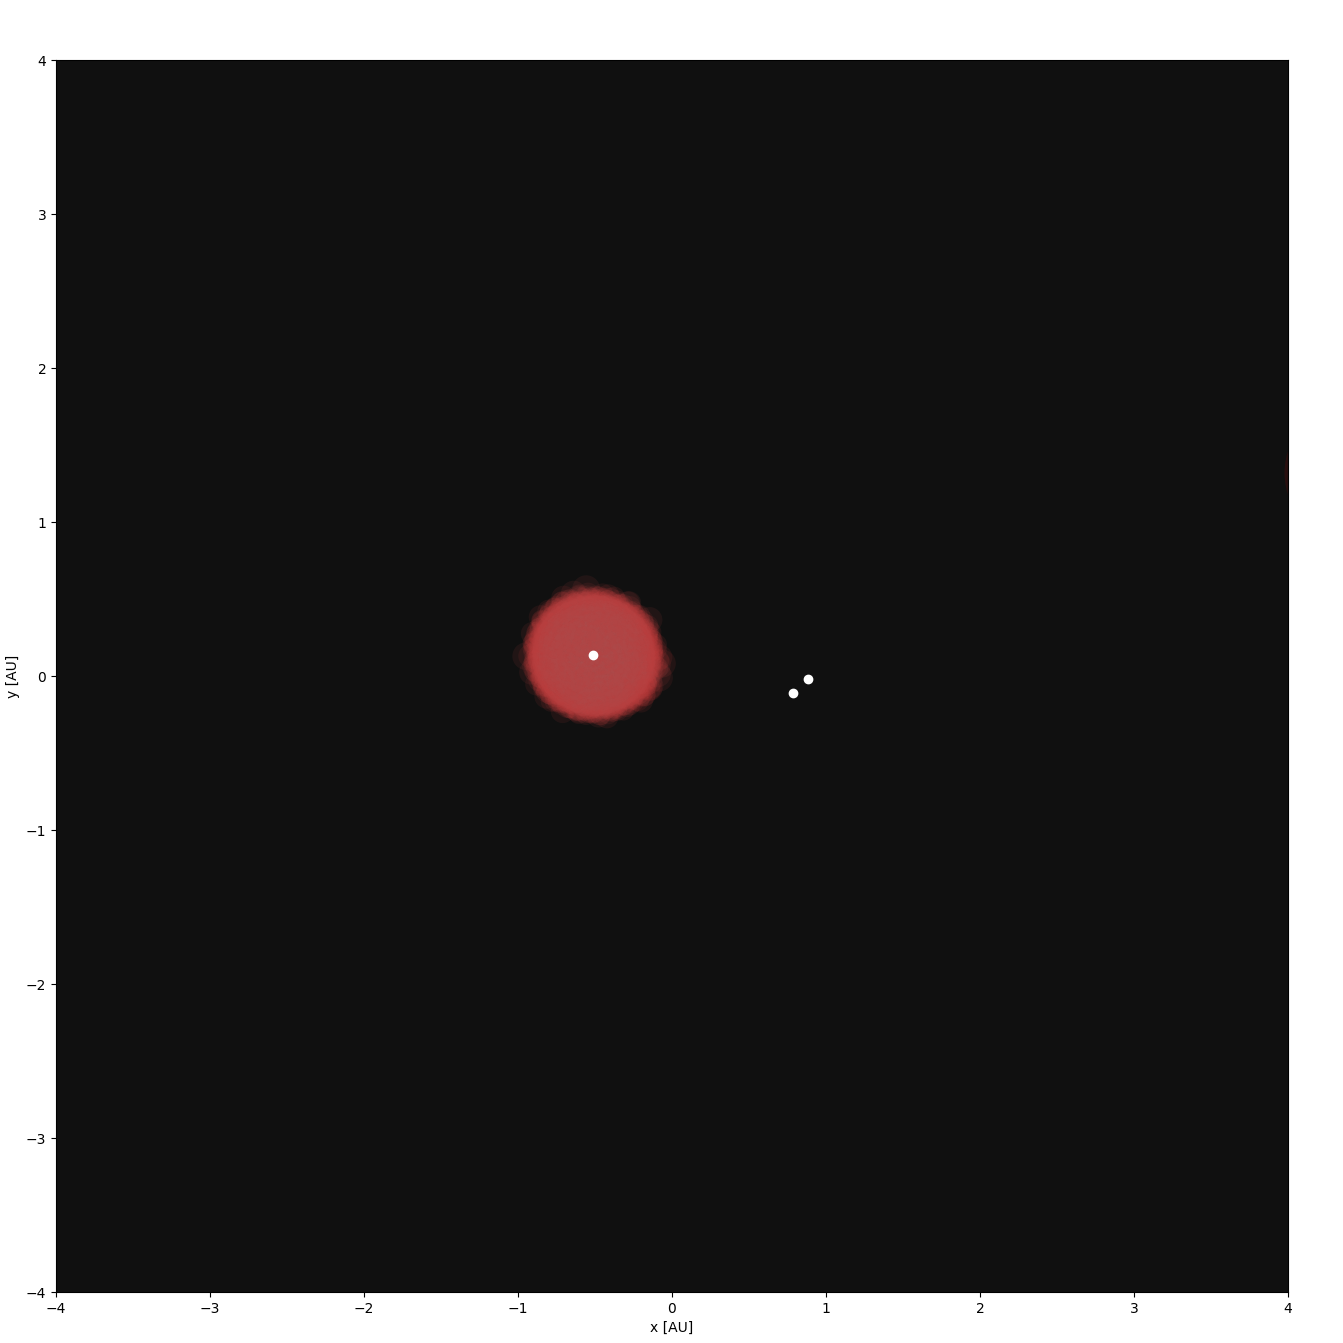
\includegraphics[width=\textwidth]{Thesis/graphs/hydro_triple_small0013687.png}   
    \end{subfigure}
    \hfill
    \begin{subfigure}[b]{0.49\textwidth}  
        \centering 
        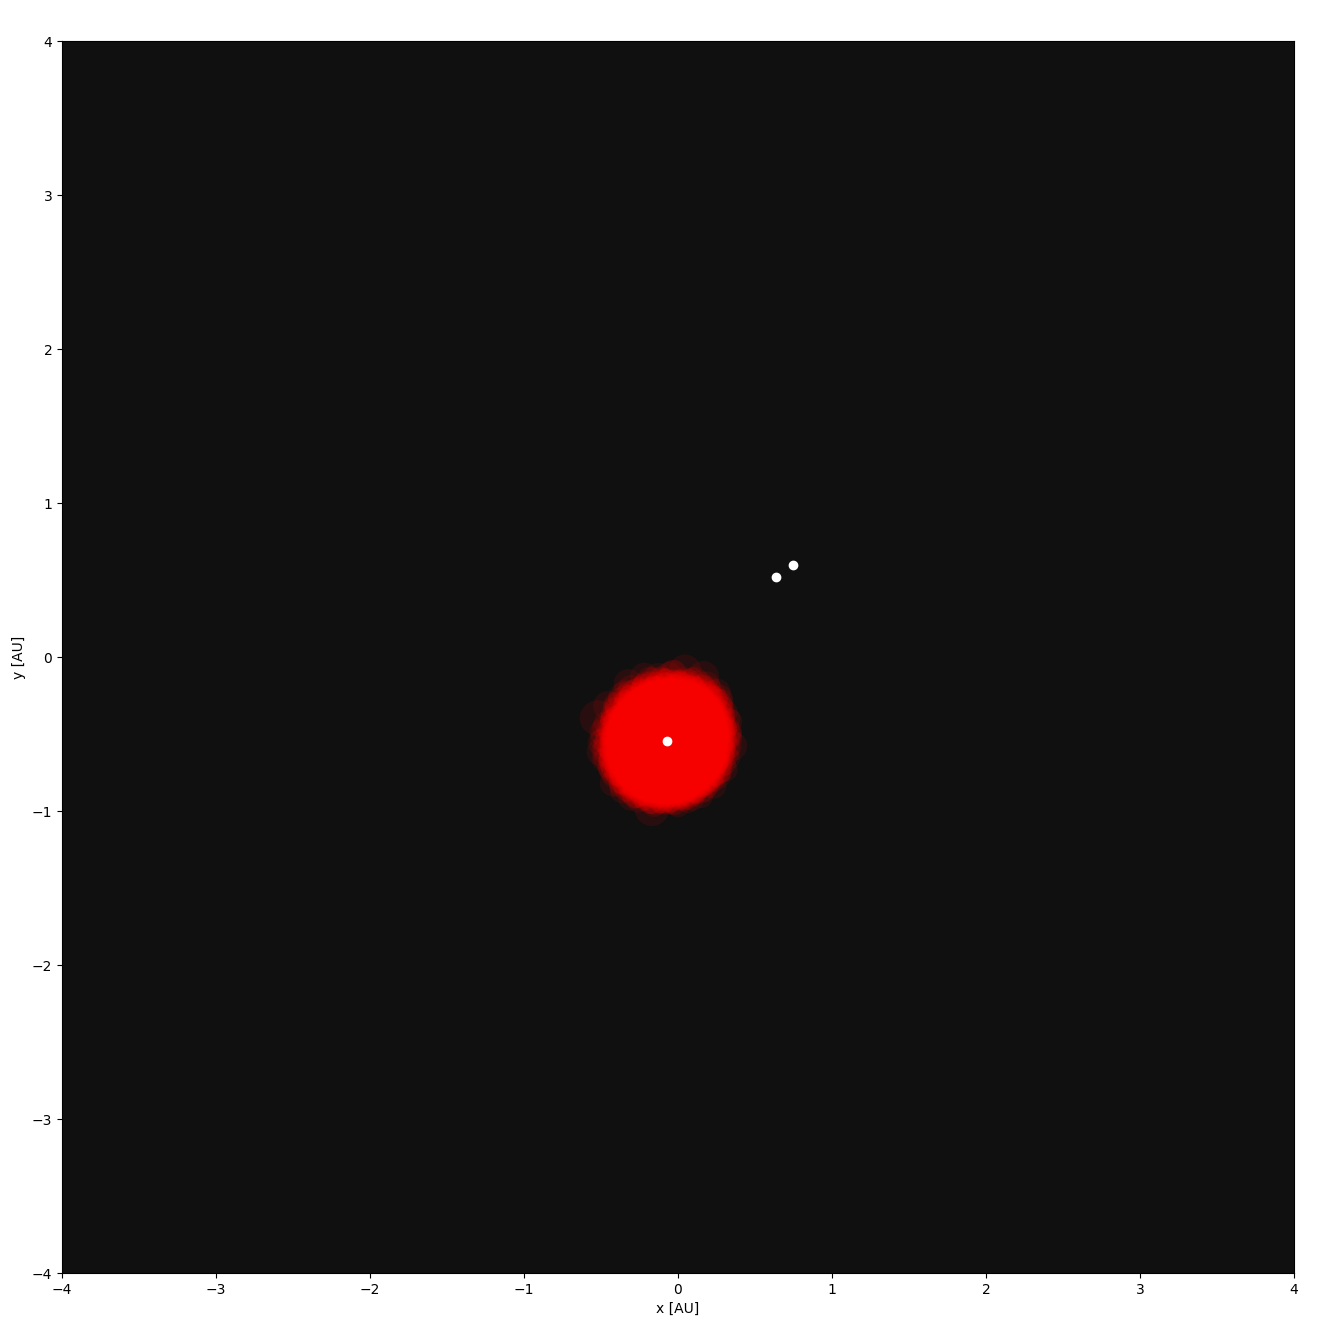
\includegraphics[width=\textwidth]{Thesis/graphs/hydro_triple_small0018250.png}
    \end{subfigure}
    \vskip\baselineskip
    \begin{subfigure}[b]{0.49\textwidth}  
        \centering 
        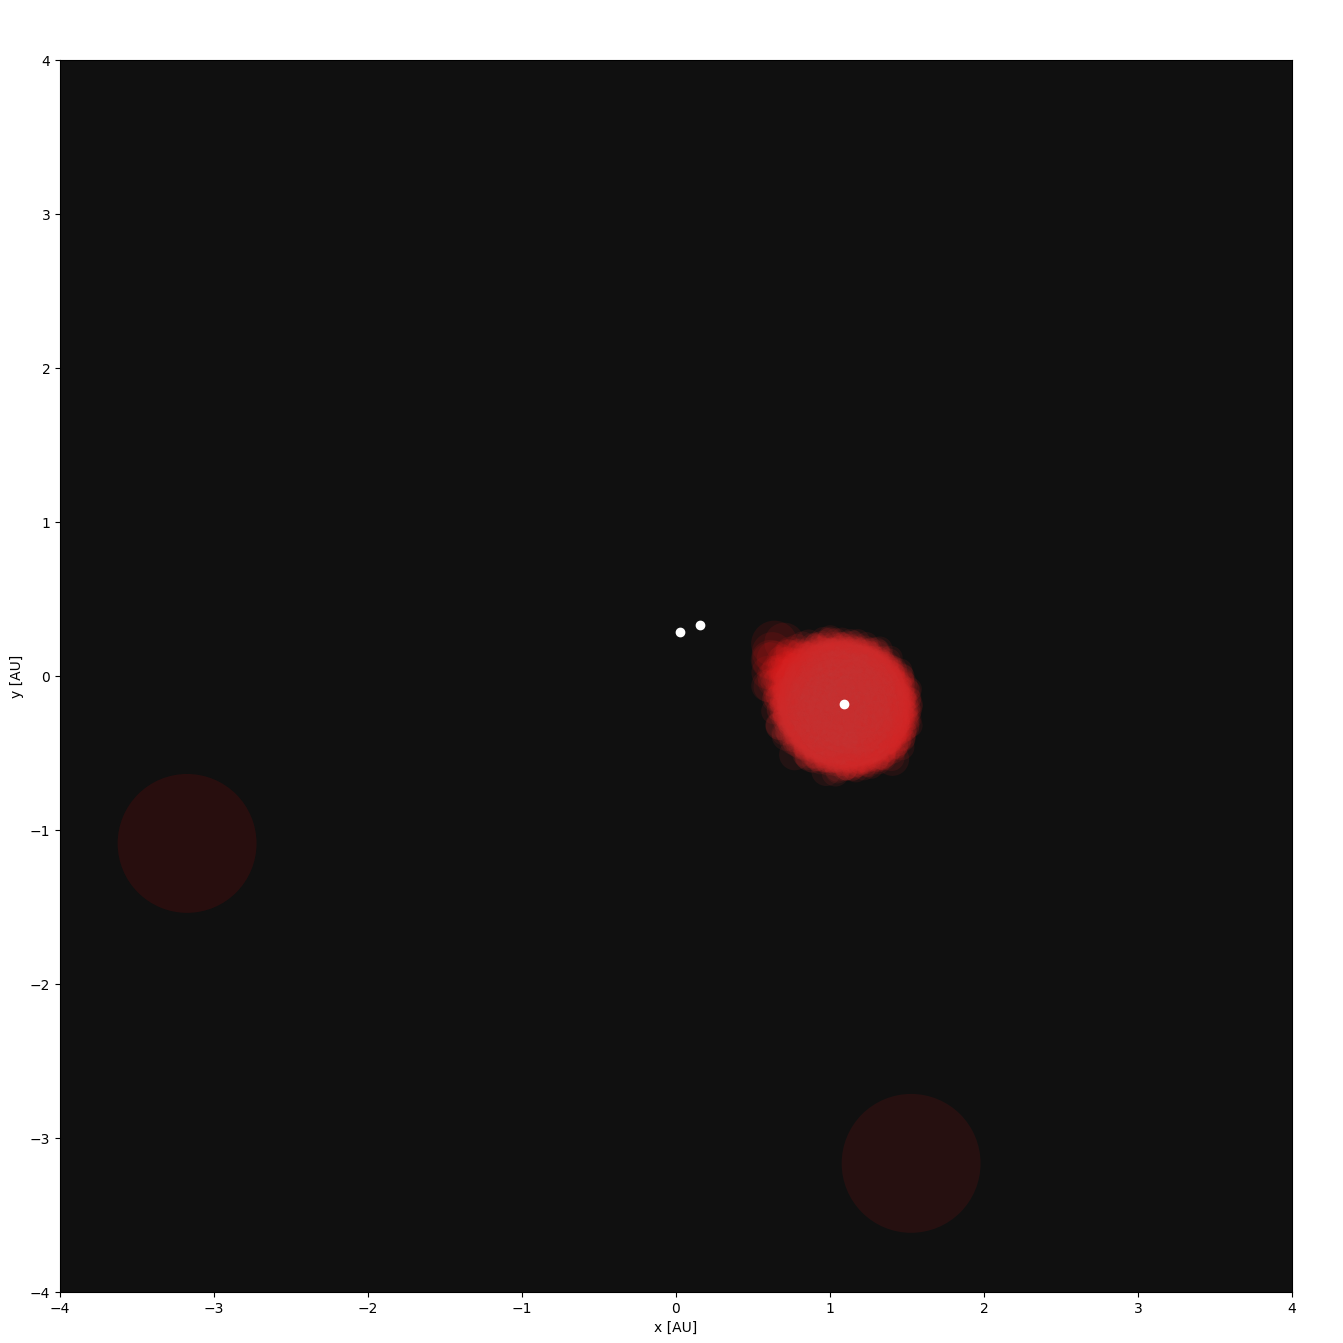
\includegraphics[width=\textwidth]{Thesis/graphs/hydro_triple_small0022812.png}
    \end{subfigure}
    \hfill
    \begin{subfigure}[b]{0.49\textwidth}  
        \centering 
        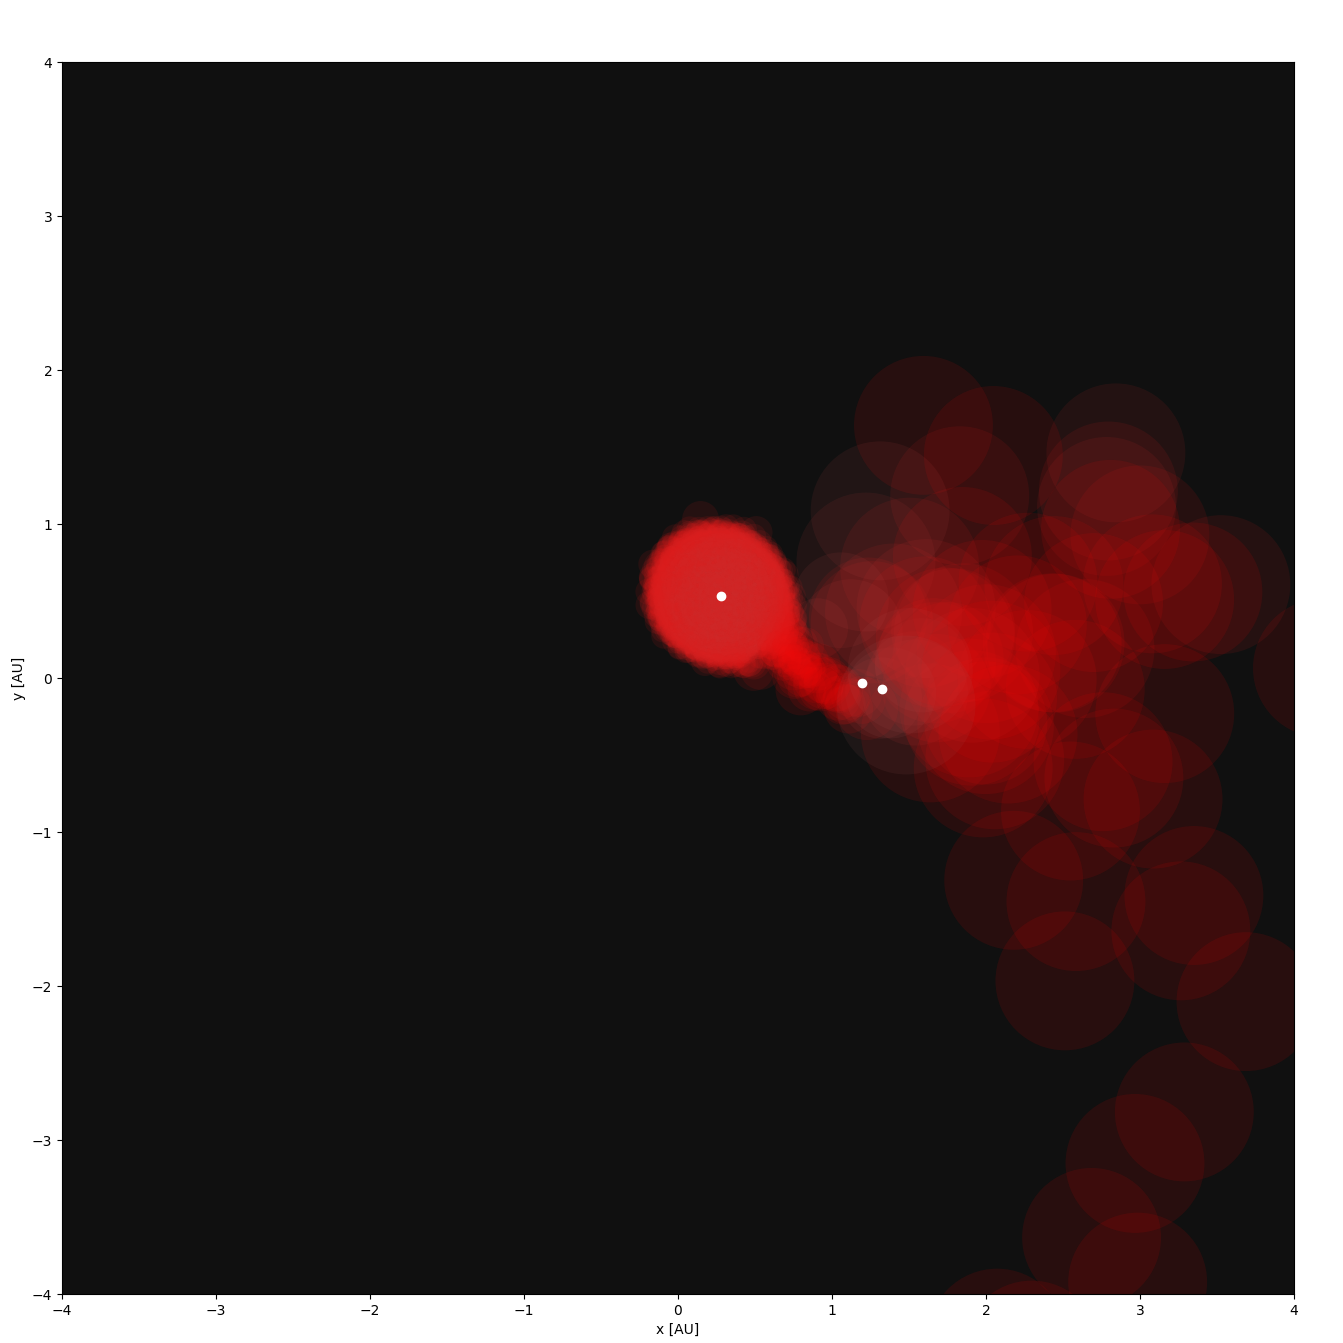
\includegraphics[width=\textwidth]{Thesis/graphs/hydro_triple_small0027375.png}
    \end{subfigure}
    \caption{System snapshots, from top to bottom and left to right, at 3.75, 5, 6.25 and 7.5 yr}
    \label{fig:simualtion_snapshots}
\end{figure}
Significant mass transfer from the tertiary towards the inner binary begins at $t \approx 4$ yr, so the time period of interest for my work begins at that point. The mass loss from the outer giant is periodic, modified by the outer orbit's periodicity, see \cref{fig:accretion_inc_00_mass_loss}. This is due to the slightly eccentric outer orbit, which causes the giant to overfill its Roche lobe at pericentre, but after semilatus rectum, the star detaches from its Roche lobe, to re-establish RLOF when it reaches pericentre again. As a result, the aforementioned periodicity is intrinsically carried through the evolution of the tertiary's mass too, see \cref{fig:accretion_inc_00_mass_loss}. Additionally, there is a significant delay between the moments of pericentre crossing and the maxima in mass transfer, see \cref{fig:simualtion_snapshots}, which is consistent with a study of RLOF in eccentric binaries \citep{lajoie2010mass}.
\begin{figure}[!htb]
    \centering
    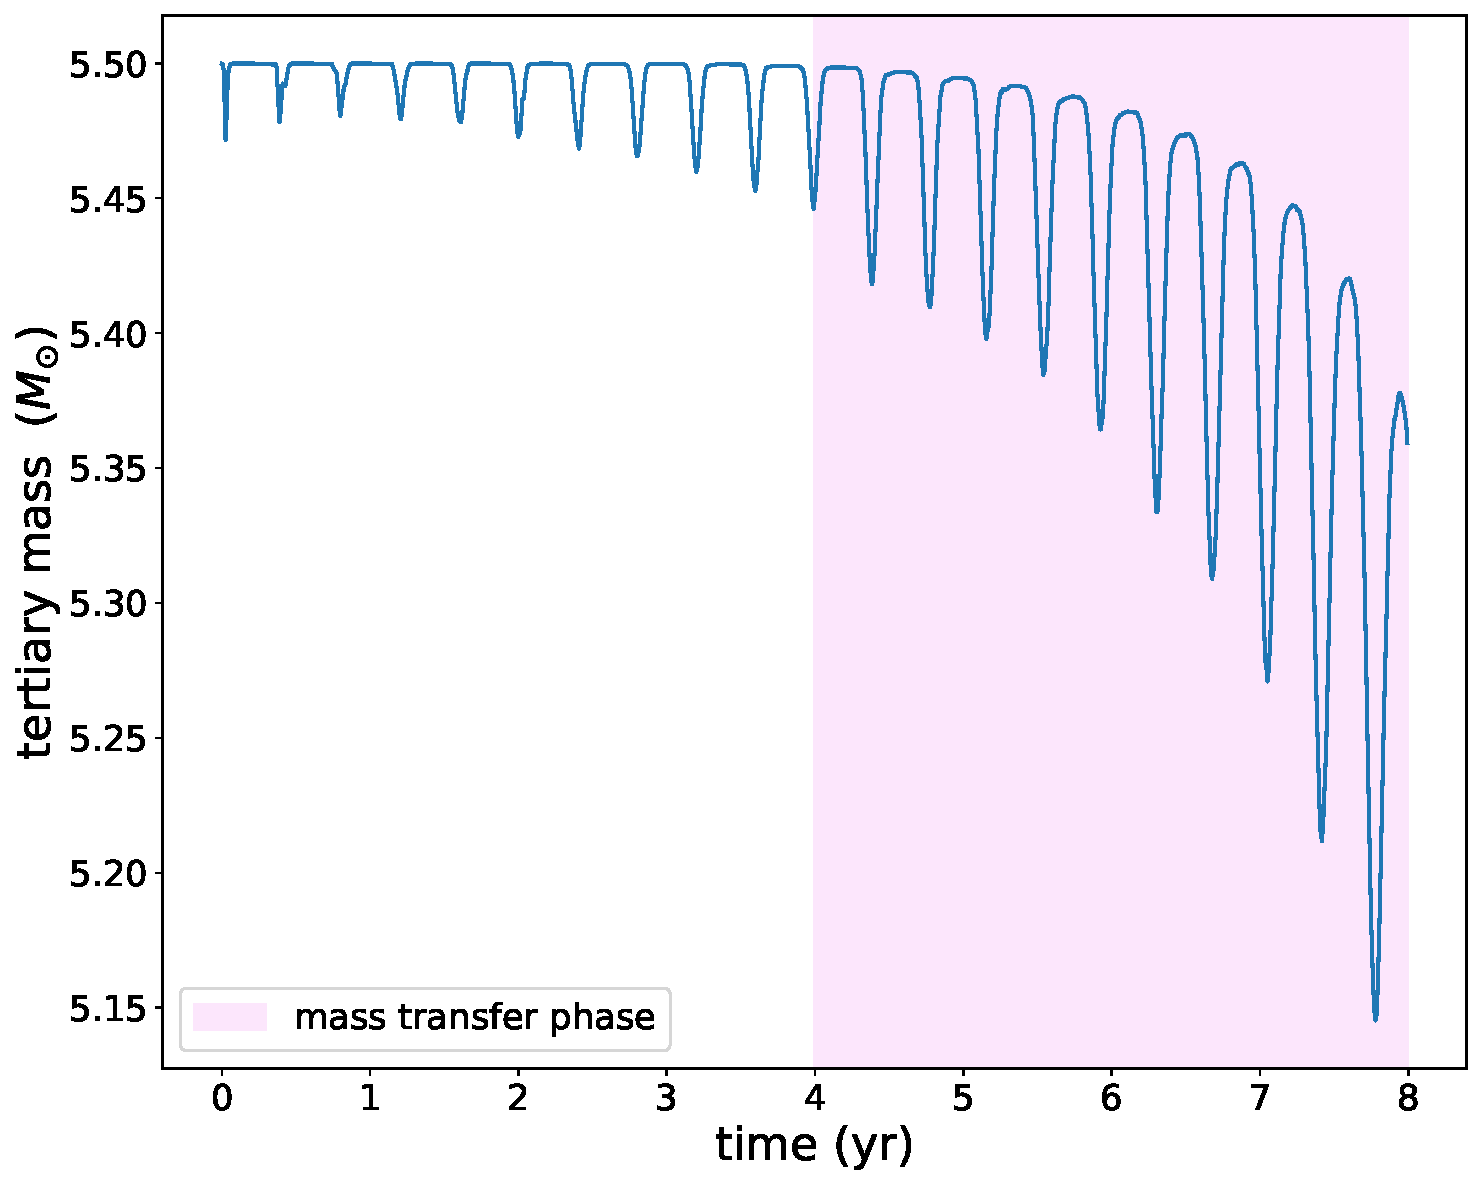
\includegraphics[width=0.85\textwidth]{Thesis/graphs/inc_00/accretion_inc_00_mass_loss.pdf}
    \caption{The evolution of the tertiary's mass.}
    \label{fig:accretion_inc_00_mass_loss}
\end{figure}
The mass transfer becomes progressively unstable, as expected for a donor with a convective envelope. Furthermore, the mass flowing from the first Lagrangian point of the outer orbit to the inner binary system interacts with the paths of the binary components. As a result, instead of a circumbinary disk, a gaseous cloud, similar to a common envelope (CE) \citep{ivanova2013common}, develops around the binary, see \cref{fig:simualtion_snapshots}. Part of the mass is being accreted by the inner binary and the rest escapes the system through the third Lagrangian point of the outer orbit, see \cref{fig:simualtion_snapshots}.

After eight years, which corresponds to $\approx 20$ orbits of the tertiary, the system enters the unstable regime, see \cref{eq:stability_regime}, and thus I terminate the simulations. Every $\delta t_{bridge}=0.1$ day, see \cref{tab:codes_settings}, I extract the mass, position and velocity of each particle in the computational domain. These properties are used to calculate the orbital parameters of the inner and the outer orbits. More specifically, the semi-major axis and eccentricity of the inner orbit are calculated using the relative position and velocity of the inner binary components. Furthermore, the relative position and velocity of the inner binary center of mass and the tertiary are used to determine the semi-major axis and eccentricity of the outer orbit. The calculations are based on \cref{eq:semi-major_axis} and \cref{eq:eccentricity}, where $M = M_1 + M_2$ and $M = M_1 + M_2 + M_3$ for orbital parameters of the inner and outer orbit, respectively. Finally, I calculate the outer orbit's relative inclination with respect to the inner orbit, i.e. mutual inclination, as the angle between their respective orbital angular momentum the vectors.

Despite being out of the scope of this work, it is worth noticing, that shortly after $t=8$ yr, the mass transfer becomes extremely unstable and a triple common envelope is encountered in all cases except for model number 3 listed in \cref{tab:simulations_settings}. For the rest models, the remainder of the tertiary's envelope engulfs the inner binary and the tertiary's core. In the case of $i_{mut} = 20^{\circ}$, the core of the tertiary is ejected from the system leaving behind a high eccentric binary. Finally, in both cases where the two orbits are initially coplanar, a direct collision completely disrupts the system.

\subsection{Outer orbit}

Tidal effects between the two orbits dominate the rates of change of orbital parameters up to $t \approx 4$ yr. The effect of mass transfer becomes visible after $t \approx 4$ years. A portion of the transferred mass is being accreted by the binary components, while the remainder is expelled from the system.  The ejected mass carries away orbital angular momentum, hence the outer orbit shrinks, see \cref{fig:accretion_inc_00_outer_semimajor_axis}. As a result,  the outer Roche lobe shrinks as well, see \cref{eq:roche_lobe}, and an increasing amount of mass can overflow towards the inner binary, see \cref{fig:accretion_inc_00_mass_loss}. 
\begin{figure}[H]
    \centering
    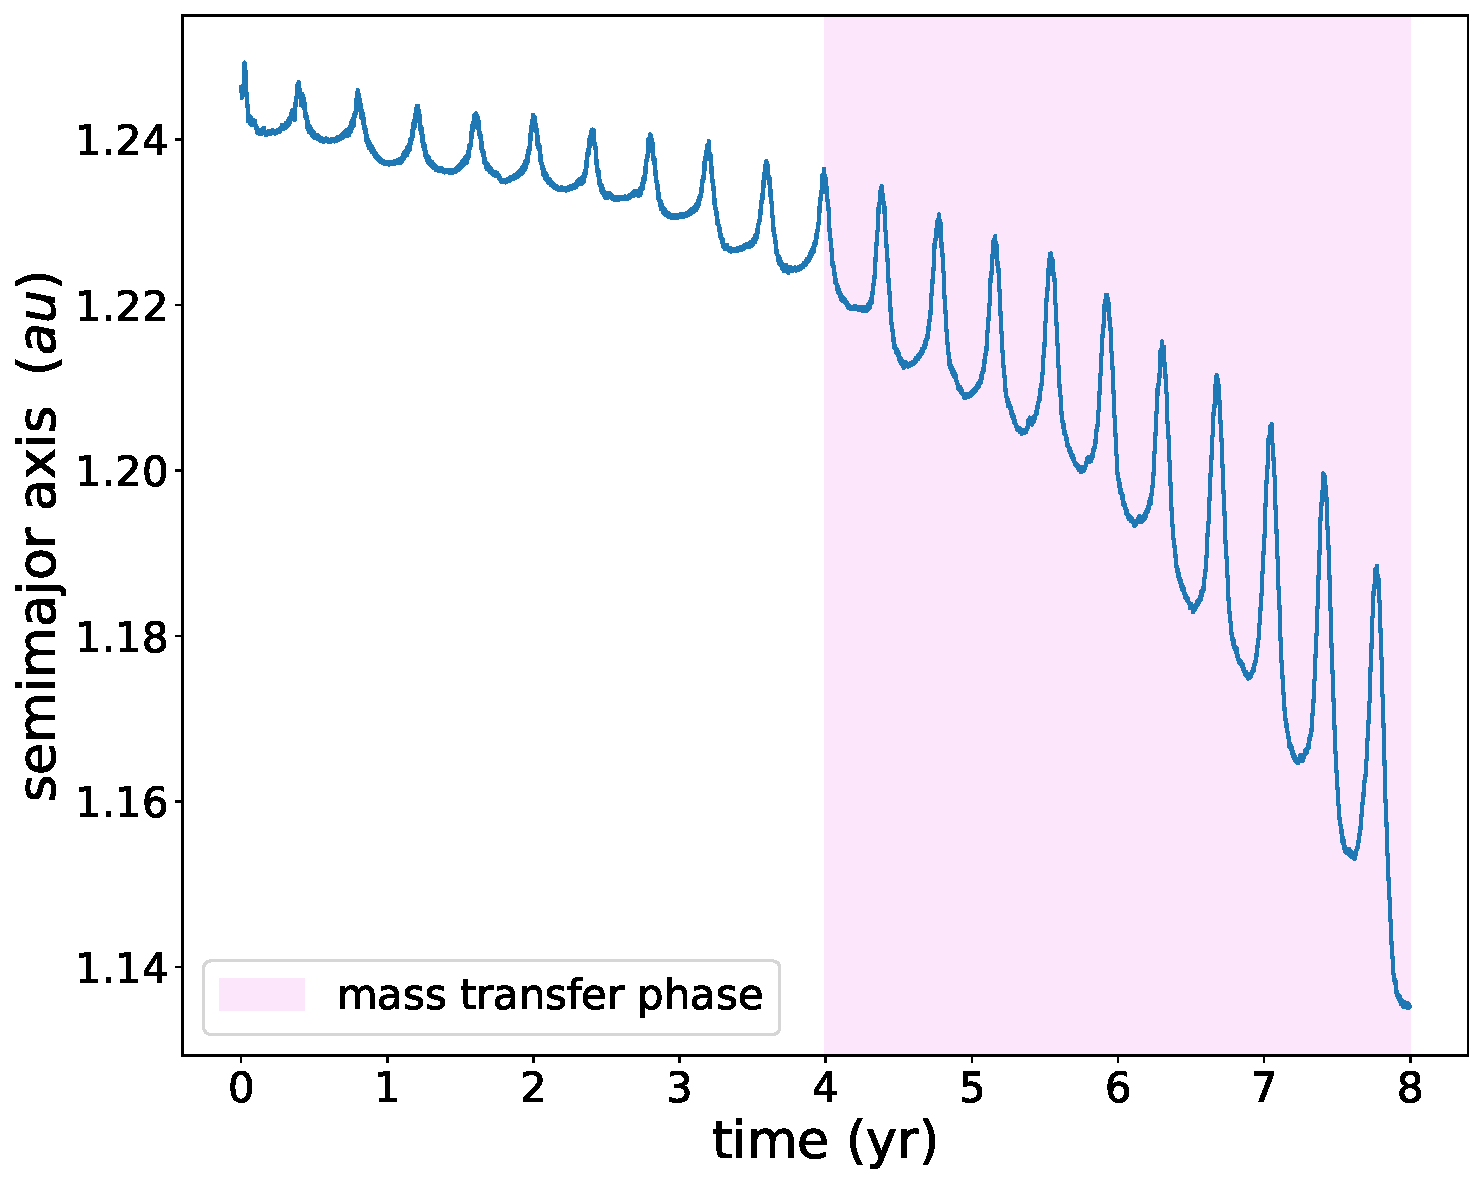
\includegraphics[width=0.85\textwidth]{Thesis/graphs/inc_00/accretion_outer_inc_00_semimajor_axis.pdf}
    \caption{Evolution of the semi-major axis of the outer orbit.}
    \label{fig:accretion_inc_00_outer_semimajor_axis}
\end{figure}
\begin{figure}[H]
    \centering
    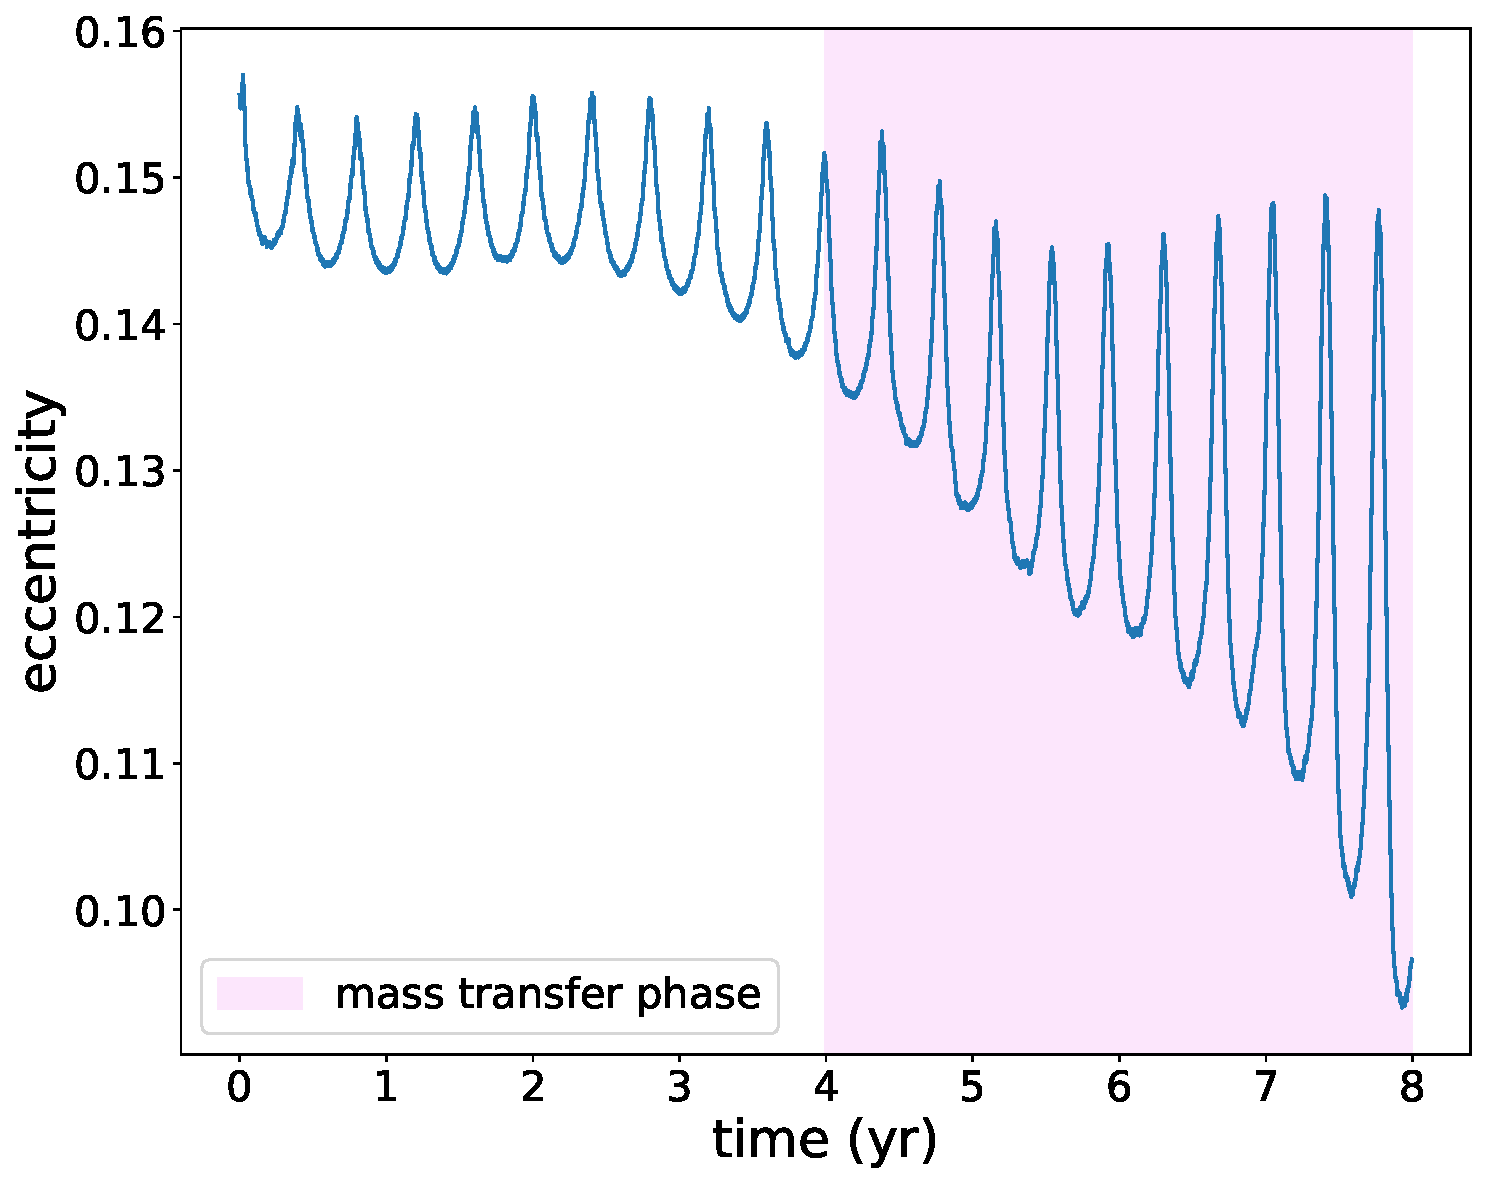
\includegraphics[width=0.8\textwidth]{Thesis/graphs/inc_00/accretion_inc_00_outer_ecc.pdf}
    \caption{Evolution of the eccentricity of the outer orbit.}
    \label{fig:accretion_inc_00_outer_ecc}
\end{figure}
\begin{figure}[H]
    \centering
    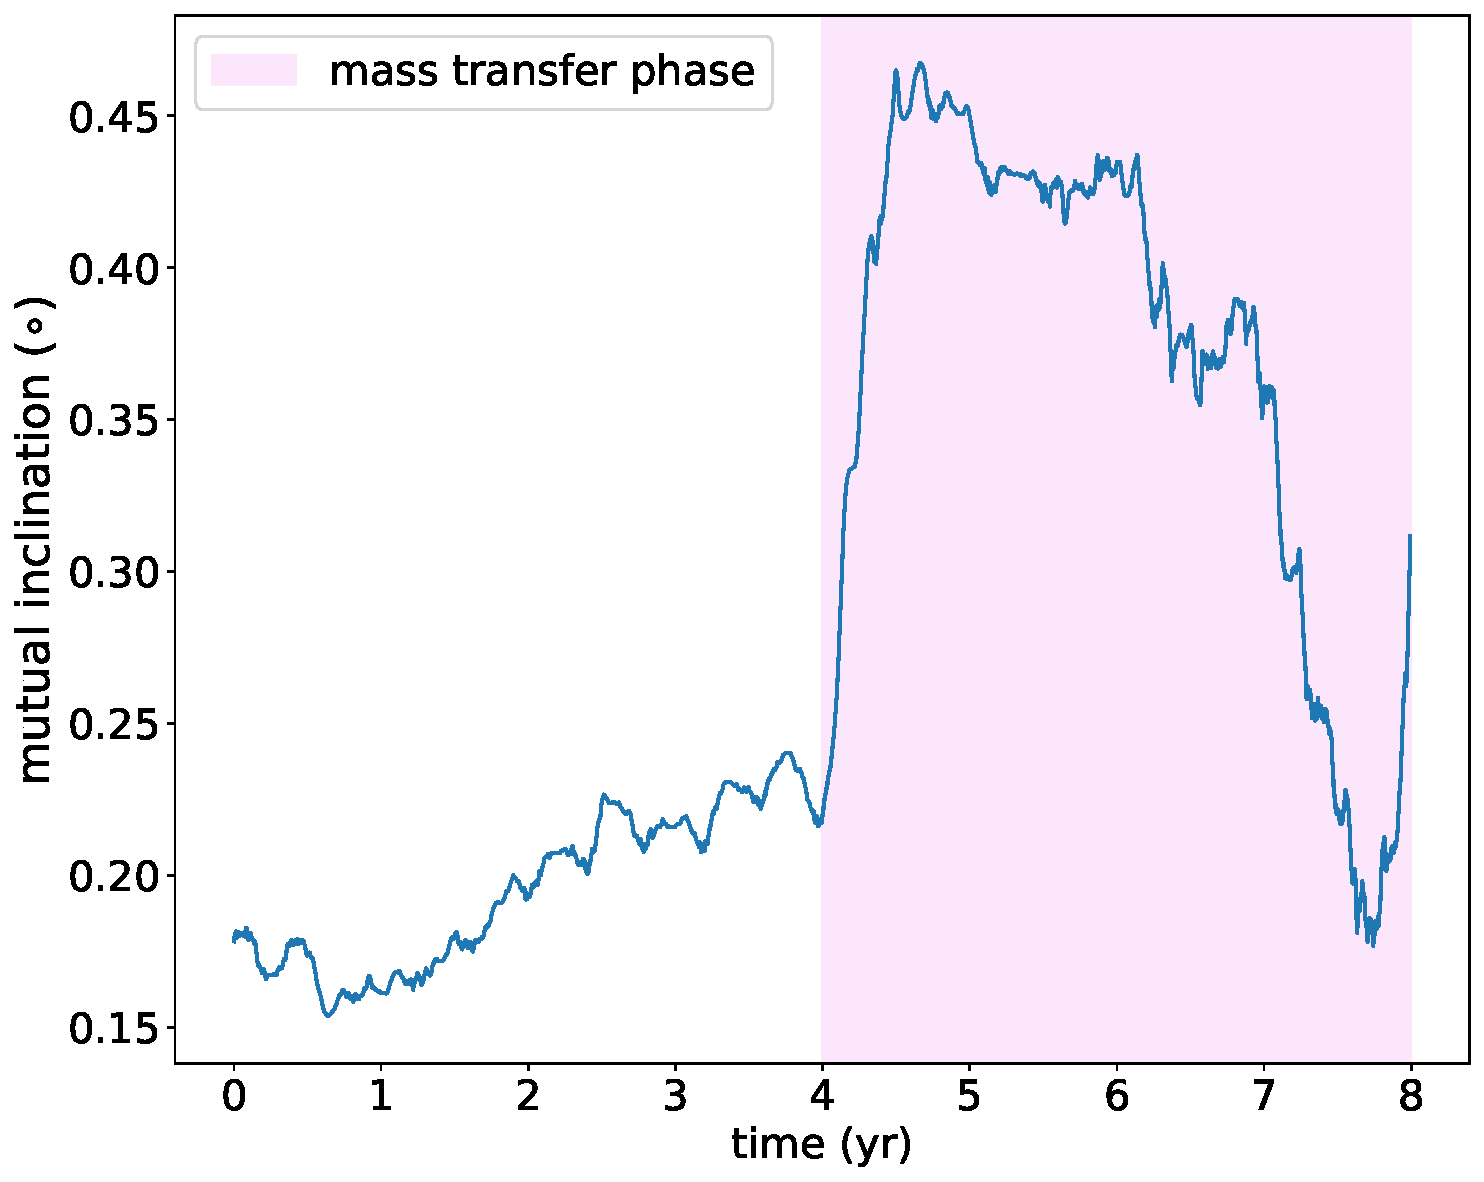
\includegraphics[width=0.8\textwidth]{Thesis/graphs/inc_00/accretion_inc_00_inc.pdf}
    \caption{Evolution of the inclination of the outer orbit relative to the inner orbit.}
    \label{fig:accretion_inc_00_inc}
\end{figure}
Furthermore, as the tertiary approaches the inner binary, tidal effects between the two orbits become stronger. Tides tend to circularize and flatten the outer orbit. \cref{fig:accretion_inc_00_outer_ecc} shows the former, while \cref{fig:accretion_inc_00_inc} shows the latter, where the outer orbit, which is already coplanar with the inner orbit, remains close to coplanarity.


\subsection{Inner orbit}

As the transferred mass intersects the inner orbit, the binary components interact with the gas. Some of the gas is being accreted, while some is ejected from the binary's close vicinity. The inner binary is generally influenced by hydrodynamics, notably gas drag, which always tends to shrink the orbit. Furthermore, by the accretion process and the inner orbit's gravitational interaction with the incoming material stream. The effect of the later on the evolution of the orbit is complex and depends on the angle at which the mass stream crosses the inner obit. This is discussed in more detail in \cref{sec:inclination}. 

In \cref{fig:accretion_inc_00_inner_semimajor_axis} and \cref{fig:accretion_inc_00_inner_ecc}, I present the evolution of the semi-major axis and eccentricity of the inner orbit, 
respectively. Both graphs show the presence of the tertiary, which introduces the observed fluctuations with periods equal to the period of the outer orbit, $\Delta t \approx 145.5$ days.
\begin{figure}[H]
    \centering
    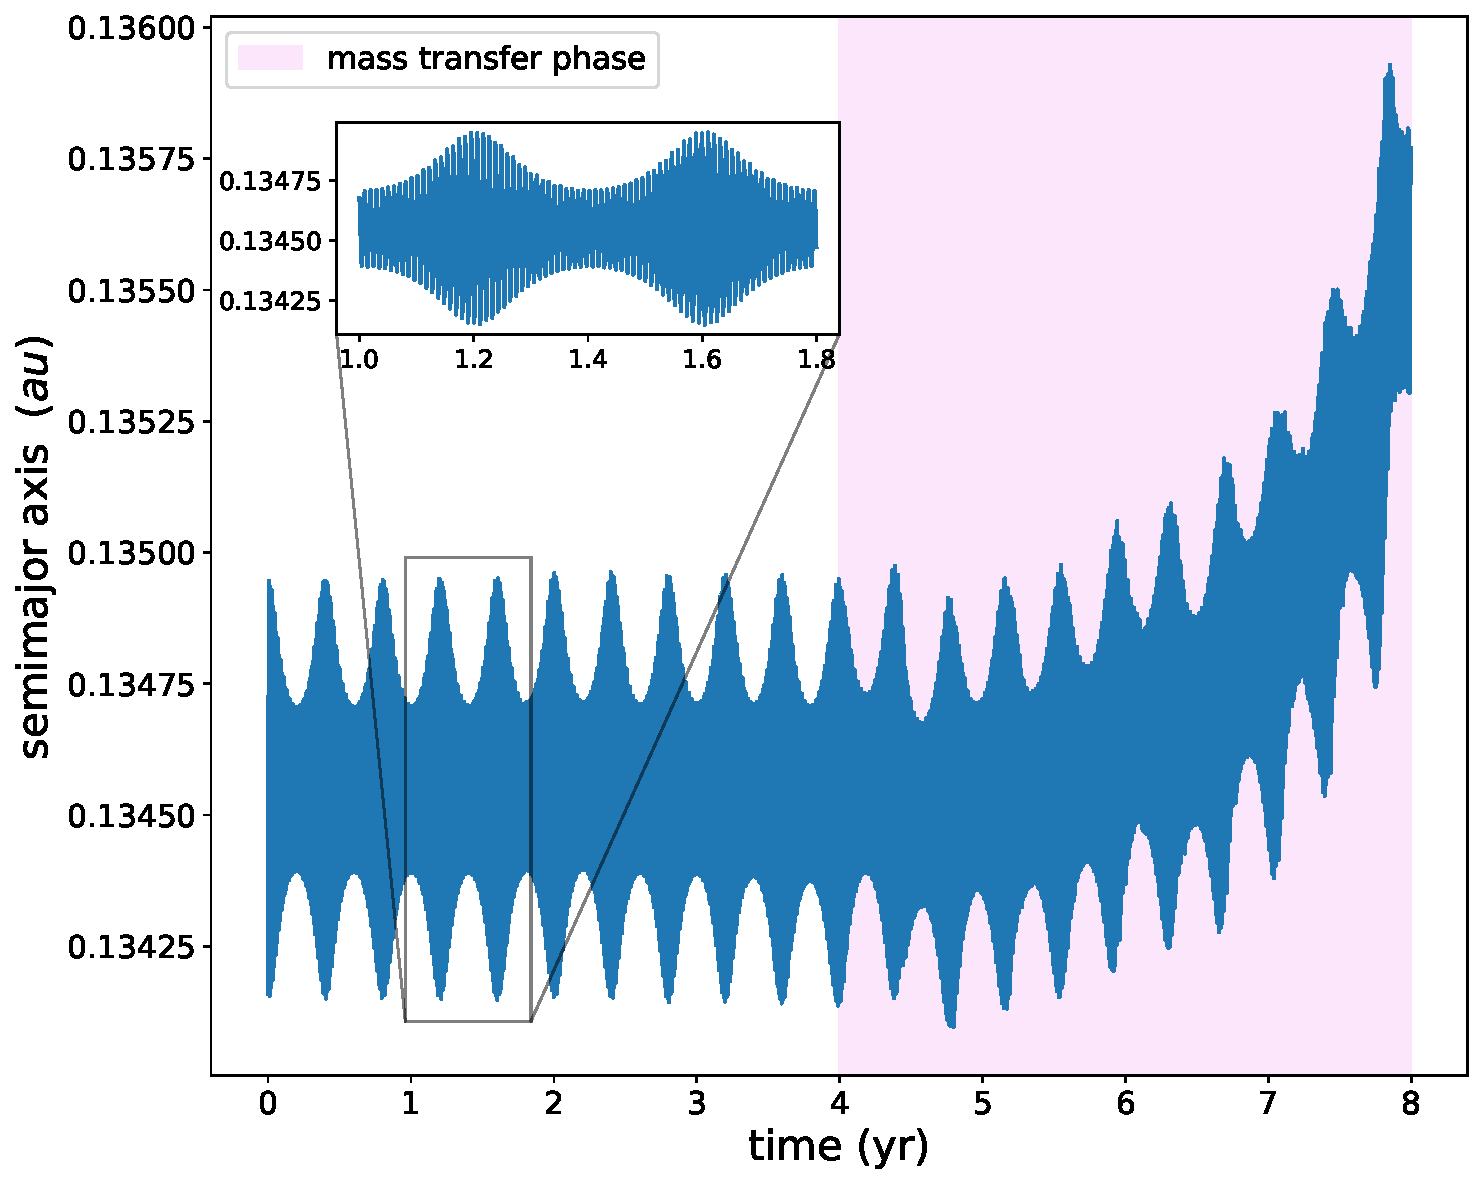
\includegraphics[width=0.9\textwidth]{Thesis/graphs/inc_00/accretion_inc_00_inner_semimajor_axis.pdf}
    \caption{Evolution of the semi-major axis of the inner orbit.}
    \label{fig:accretion_inc_00_inner_semimajor_axis}
\end{figure}
In the case where the inner and outer orbit are coplanar the former seems to widen, see \cref{fig:accretion_inc_00_inner_semimajor_axis}. 
This is an unexpected outcome, because a common envelope-like structure around the binary is encountered and a detailed discussion is taking place in \cref{sec:resolution}. Furthermore, the effect of mass transfer on the eccentricity of the inner orbit is negligible and the orbit remains circular. 
\begin{figure}[!htb]
    \centering
    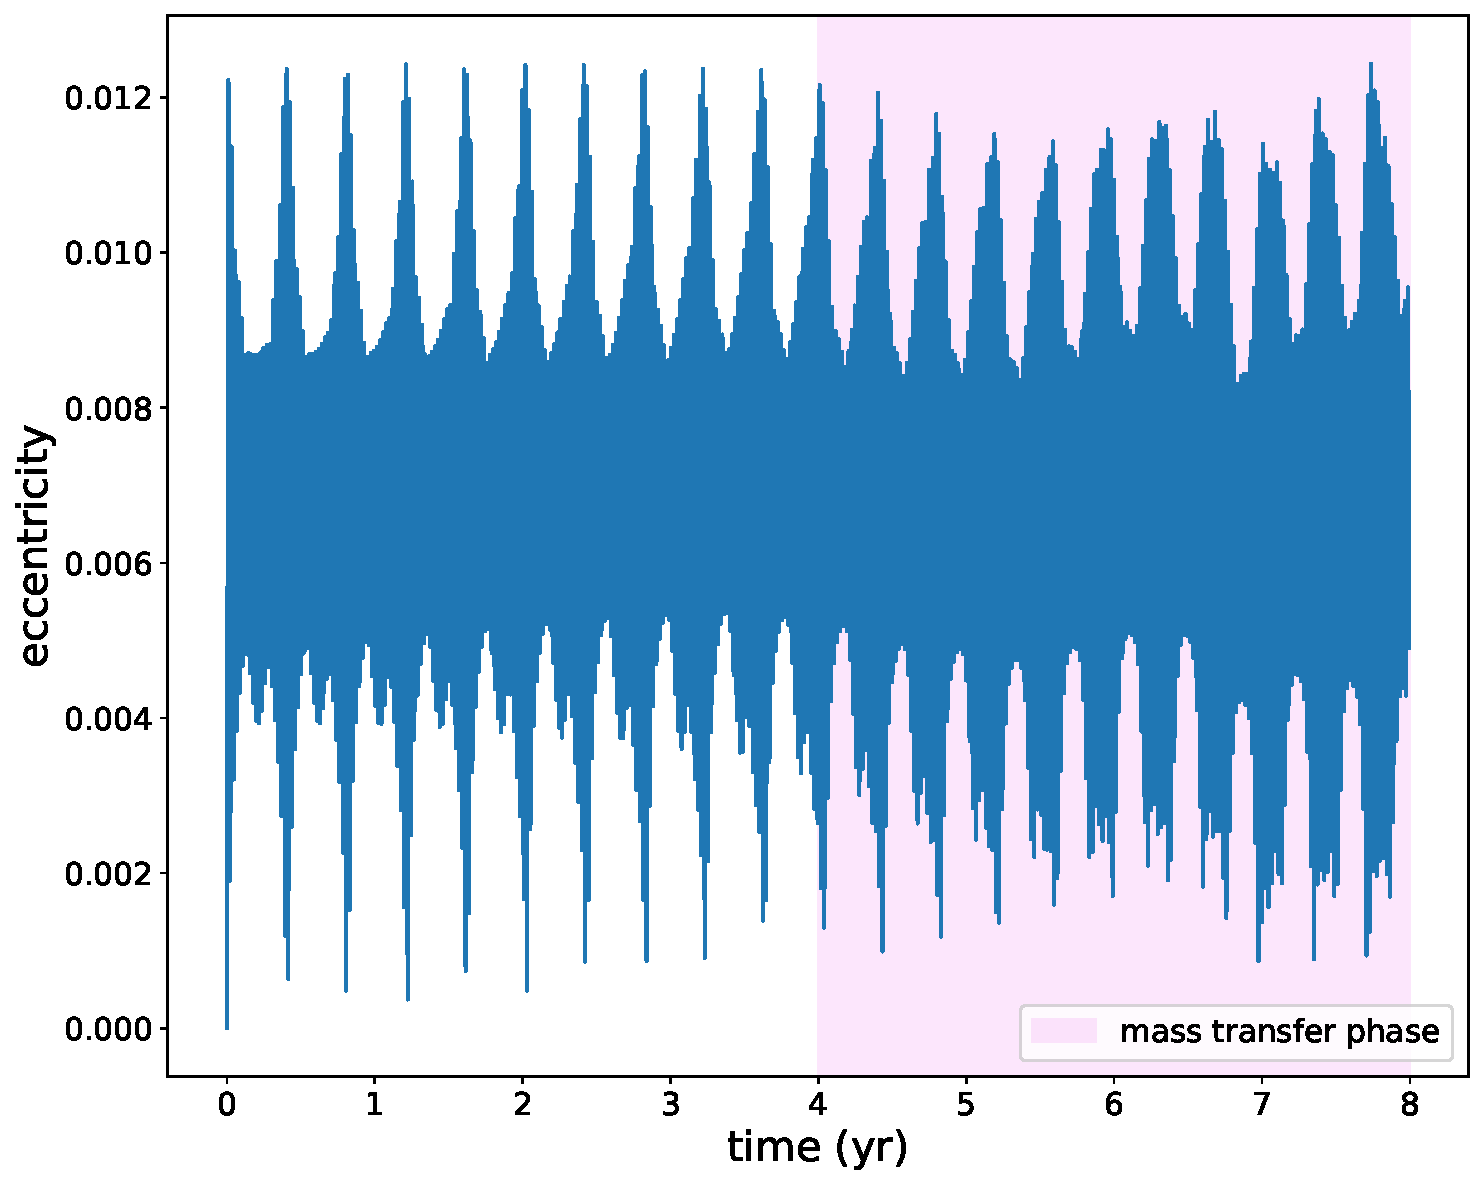
\includegraphics[width=0.9\textwidth]{Thesis/graphs/inc_00/accretion_inc_00_inner_ecc.pdf}
    \caption{Evolution of the eccentricity of the inner orbit.}
    \label{fig:accretion_inc_00_inner_ecc}
\end{figure}




\section{Resolution Benchmark}\label{sec:resolution}

In the general case of RLOF by an outer star towards an inner binary, the response of the latter's orbit may vary. \cite{zwart2019triple} investigate the case in which the incoming mass stream forms a circumbinary disk. They find that the details of the accretion can cause the inner orbit to shrink, a behavior that reverses though assuming a more massive donor. In the case where a common envelope-like structure is formed around the inner binary, the orbit is expected to shrink \citep{de2014evolution}. Given that the efficiency of the gas drag in shrinking the inner orbit must be strongly related to the density of the gas cloud surrounding the inner binary, I need to investigate whether the observed behavior, see \cref{fig:accretion_inc_00_inner_semimajor_axis}, is a physical result or the result of poor resolution (small number of SPH particles).

The smoothing length is determined by the number of SPH particles in a region of the computational domain, which in turn defines the simulation's resolution in that region, see \cref{sub:gadget2}. The latter is small in high-density regions and large in low-density regions. To correctly account for the influence of gas drag on the inner binary, the smoothing length of the particles interacting with it must be considerably smaller than the binary's size. In my simulations, $N=50000$ is used. 

A simulation's snapshot at $t \approx 7.5$ yr is illustrated in \cref{fig:resolution}, where the mass transfer is maximum. The x-axis represents the distance of each particle from the tertiary's center of mass, while the y-axis represents the smoothing length of each particle. The horizontal yellow line corresponds to the orbital separation of the inner binary components, i.e. the binary's size. Finally, the red area represents an approximation of the inner binary's close vicinity. More specifically, it corresponds to the position of the inner binary's center of mass $\pm$ the binary's size.
\begin{figure}[!htb]
    \centering
    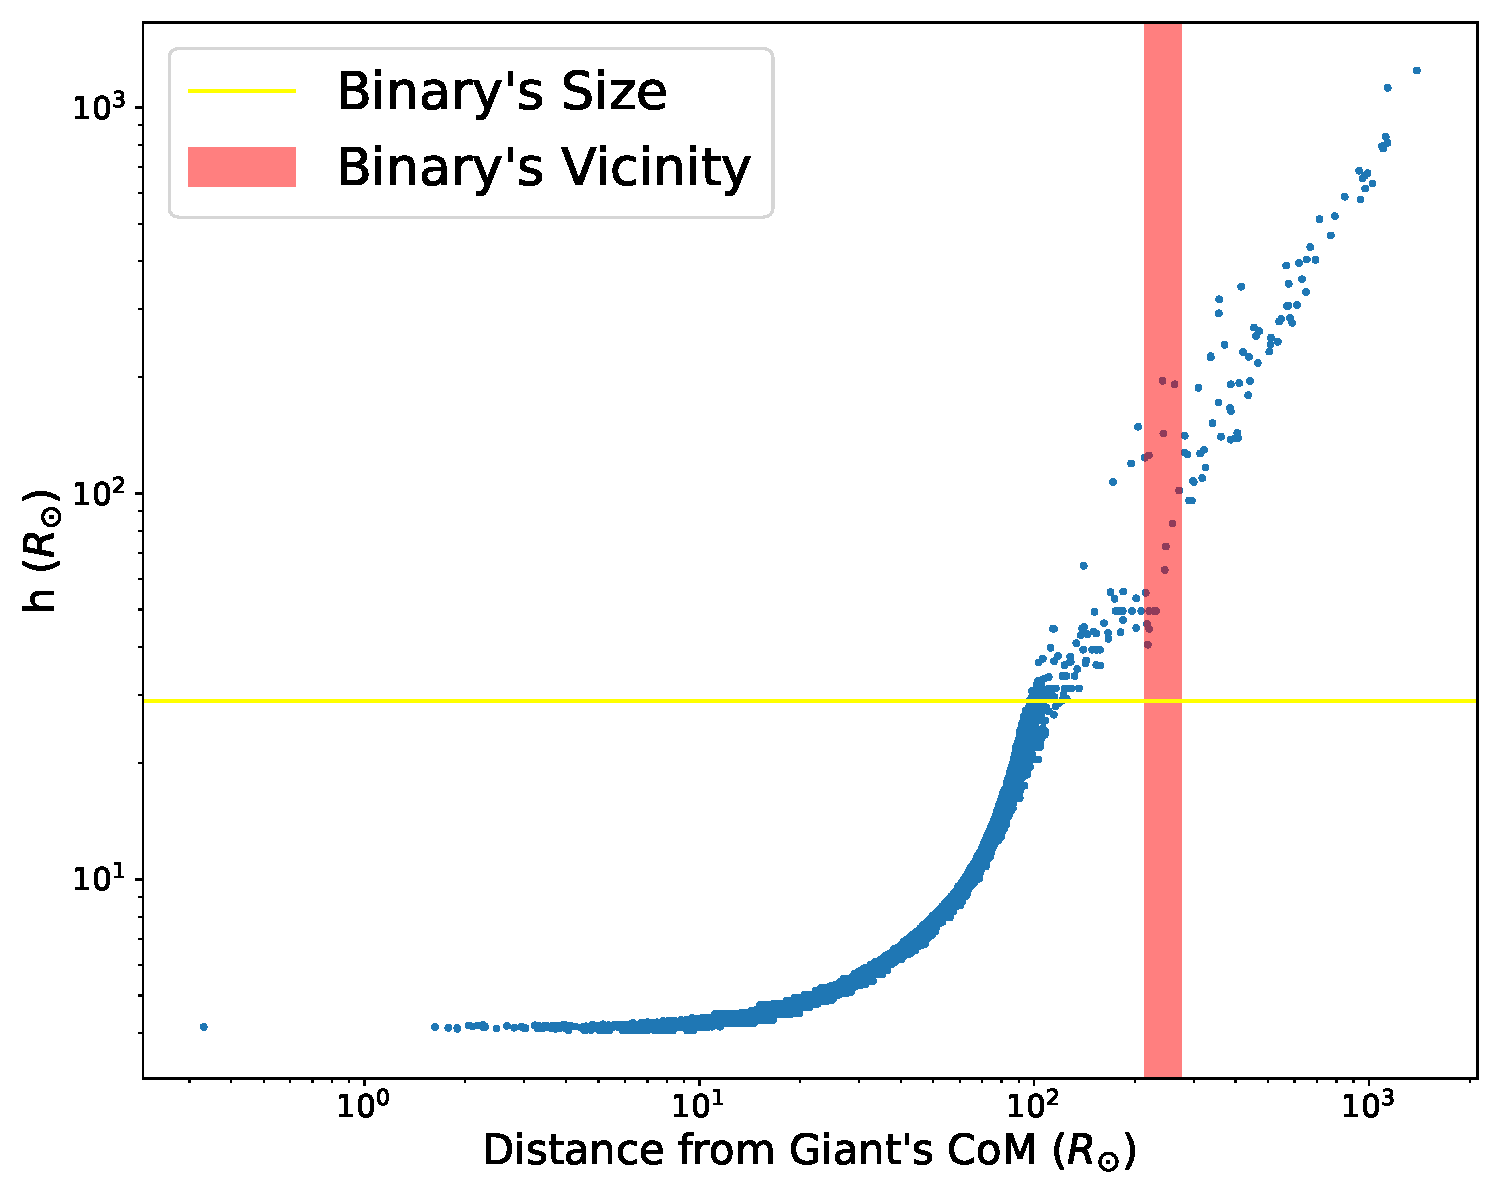
\includegraphics[width=0.9\textwidth]{Thesis/graphs/resolution_benchmark.pdf}
    \caption{Particles smoothing lengths in comparison to the binary's size at $t \approx 7.5$ yr, where the mass transfer is maximum.}
    \label{fig:resolution}
\end{figure}

Particles with smoothing lengths smaller than the binary's size, blue points bellow the yellow line, and close to the binary, blue points close/inside the red region, can influence hydrodynamically the inner orbit. At the current resolution, even when the mass transfer is maximum, the number of particles interacting with the binary is small (low-density mass stream), and thus their smoothing length is much larger than the size of the inner orbit, hence the present resolution probably underestimates the effect of gas drag. In conclusion, higher resolution simulations are required to safely estimate the evolution of the semi-major axis of the inner orbit.

Given the underestimation of gas drag and the resulting development depicted in \cref{fig:accretion_inc_00_inner_semimajor_axis}, I ran a test simulation in which the initial inner and outer orbital angular momentum vectors are antiparallel. In the parallel case, see orange line in \cref{fig:retro}, accretion and gravitational interactions between the stars and the incoming mass stream appears to work as a slingshot effect in favor of the stars. Whereas in the antiparalel scenario, it appears to act as a braking mechanism for the stars, see blue line in \cref{fig:retro}. The reason behind this behavior is the following: When a sink accretes a gas particle, its mass and momentum are added to the star. Because momentum is a vector, the acceleration or deceleration of the star must be determined by the relative vector of the star's and the particle's velocity. This implication explains the observed trend in \cref{fig:accretion_inc_00_inner_semimajor_axis} and it is further investigated in \cref{sec:inclination}.
\begin{figure}[!htb]
    \centering
    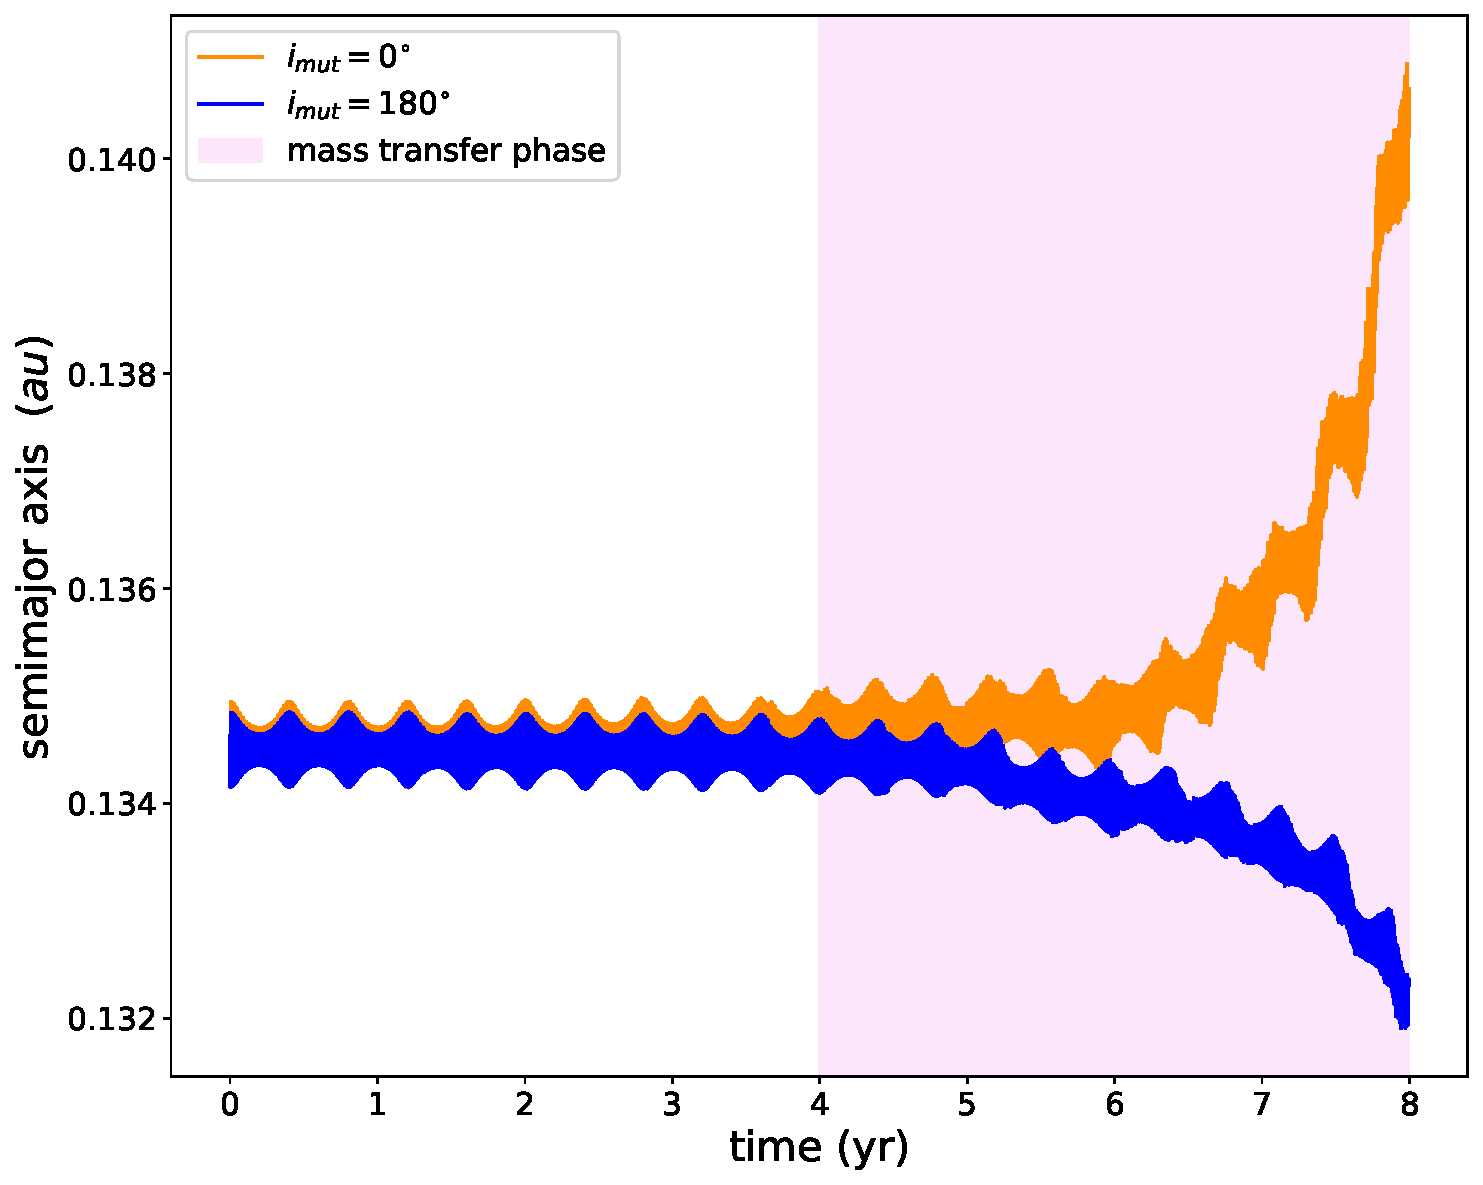
\includegraphics[width=0.9\textwidth]{Thesis/graphs/accretion_inc_00_retro_inner_semimajor_axis.pdf}
    \caption{Evolution of the semi-major axis of the inner orbit. The orbital angular momentum of the inner and outer orbit are parallel and antiparallel for the the orange and blue lines, respectively.}
    \label{fig:retro}
\end{figure}

Despite the fact that $N=50000$ is sufficient to initially resolve the giant at the moment of RLOF, see \cref{sec:1D_to_3D}, it is insufficient to accurately capture the gas drag on to the inner orbit. The fact that \cite{de2014evolution} use also $N=50000$ to examine mass transfer via RLOF by the outer star, for the same system was a motivation behind this particular choice. In their study, they employ a different SPH code. Nevertheless, both codes define the particles smoothing length in a similar fashion, thus it is a surprise that they are able to account for gas drag at seemingly the same resolution. 

To achieve higher resolution, I could simply increase the number of particles in my simulation. This is pretty straight forward in my code, however time restrictions require me to consider leaving this for future work. More specifically, with the available computational resources I obtain eight years of simulation in approximately five weeks of computational run time. Considering that the CPU time scales with the number of \ac{sph} particles as $NlogN$, increasing the number of particles by a factor of 5 results in several months of computational run time. 

In conclusion, with the current number of \ac{sph} particles the resolution of my simulations is probably insufficient to accurately capture the influence of the gas drag on the inner orbit. As a result, the gas drag is underestimated, while the models capture the gravitational interactions between the inner binary, the core of the tertiary, and its gaseous envelope. Regardless, I can still extract useful information about the evolution of the outer orbit and conjecture about the evolution of the inner orbit. 

\section{Impact of accretion}\label{sec:accretion}

In this section, I compare models  1 \& 4 listed in \cref{tab:simulations_settings}, which correspond to the maximum and minimum accretion case, respectively. Here, I examine the effects of accretion on the evolution of the system.

In \cref{sec:mass_transfer_RLOF}, I showed that periodic variations are naturally integrated in my models due to the outer orbit's eccentricity. The key point though, is that the timescale of this periodicity is equal to the period of the outer orbit. In the parent and next section, I focus on the global evolution of the orbital parameters. As a result, the presented graphs associated with the outer orbit, display not only the original output of my simulations, but also smoothed versions of it. A kernel of width equal to $3 \times P_{out}$ is used to smooth the data. The is for illustration purposes only, as it is easier for the reader to follow the comparison between the models listed in \cref{tab:simulations_settings}. 

\subsection{Outer orbit}

In \cref{fig:accretion_outer_semimajor_axis}, \cref{fig:accretion_outer_ecc} and \cref{fig:accretion_inc}, I display the evolution of the semi-major axis, eccentricity and the inclination of the outer orbit relative to the inner orbit, respectively.

For the minimum accretion case, the outer orbit decays faster, see \cref{fig:accretion_outer_semimajor_axis}. This behavior is expected, because more mass is lost from the system and the ejected mass carries away orbital angular momentum. Furthermore, as the tertiary approaches the inner binary, tidal effects between the two orbits become stronger. Tides tend to circularize and flatten the outer orbit. More specifically, in the equilibrium-tide model, the circularization timescale is $\propto \frac{R_{\star}}{\alpha}^{-8}$ and the faster decay of the orbit leads to a faster circularization too, see \cref{fig:accretion_outer_ecc}. Finally, in both cases, the outer orbit, which is already coplanar with the inner orbit, remains close to coplanarity, see \cref{fig:accretion_inc}.
\begin{figure}[H]
    \centering
    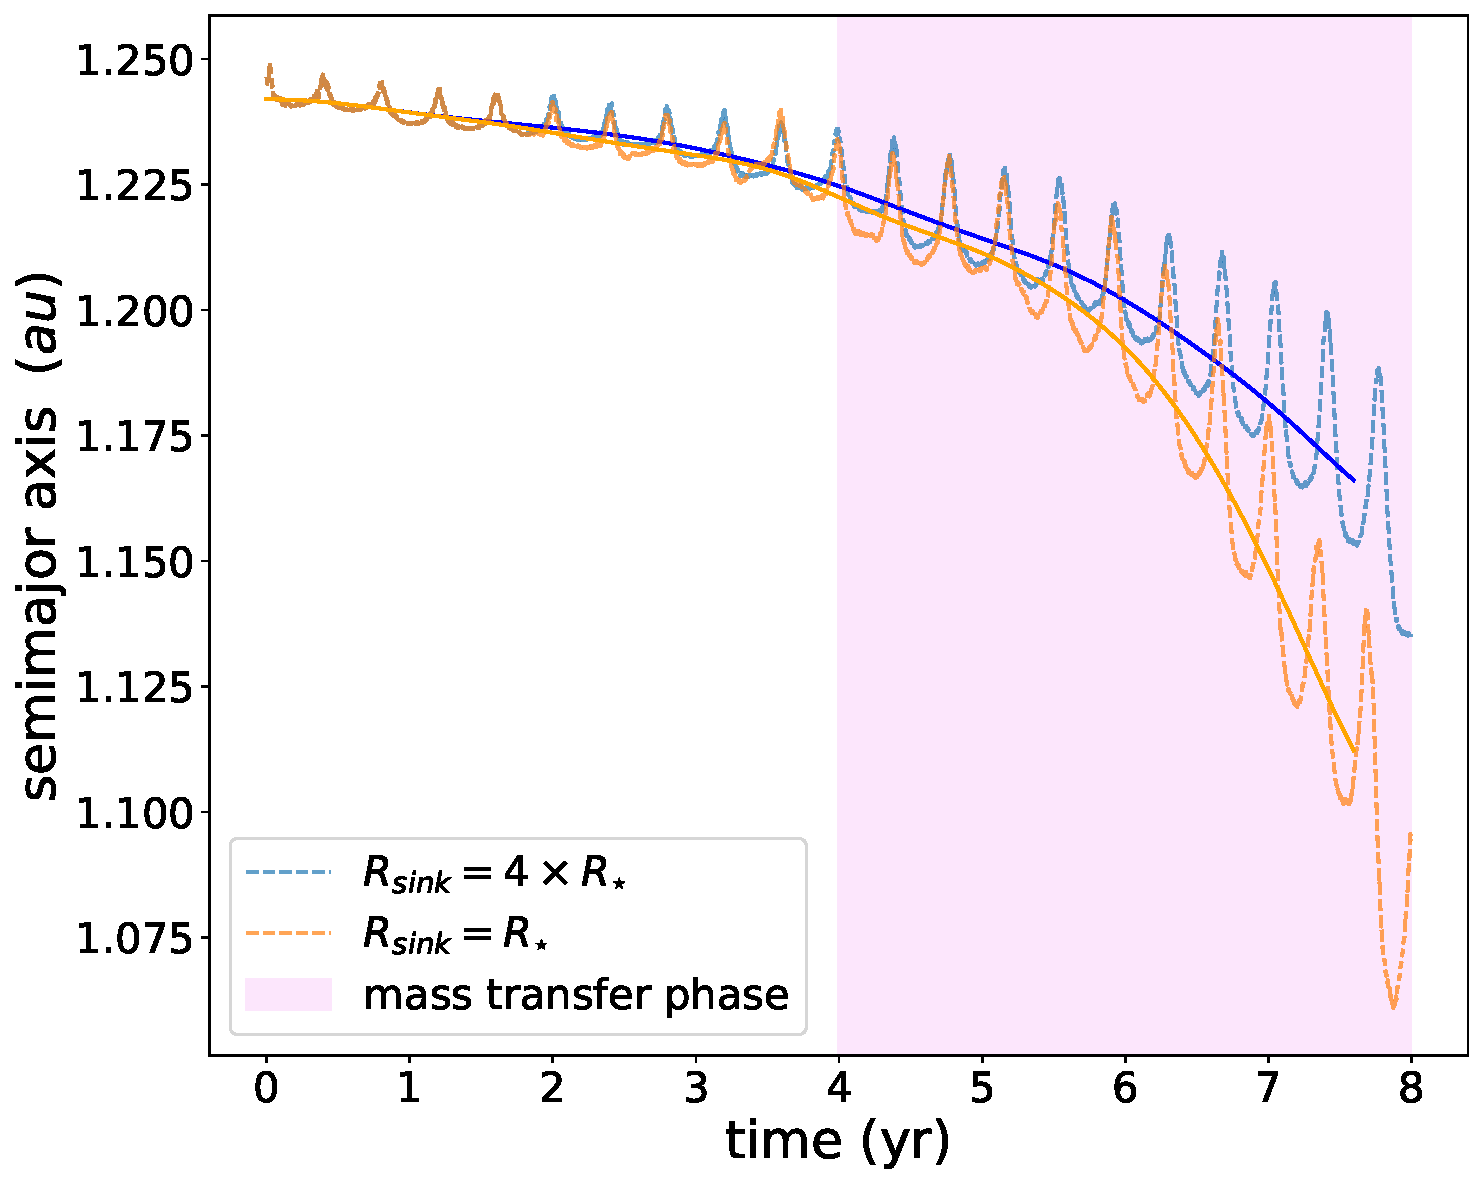
\includegraphics[width=0.9\textwidth]{Thesis/graphs/accretion_case/accretion_outer_semimajor_axis.pdf}
    \caption{Evolution of the semi-major axis of the outer orbit for the minimum and maximum accretion case. The simulated data is shown in dashed lines. The continues lines are smooth representations of the simulated data in their respective colors. The last three orbits are not included in the smoothed version, because the lack of data above $8$ yr will erroneously flatten the slopes.}
    \label{fig:accretion_outer_semimajor_axis}
\end{figure}
\begin{figure}[H]
    \centering
    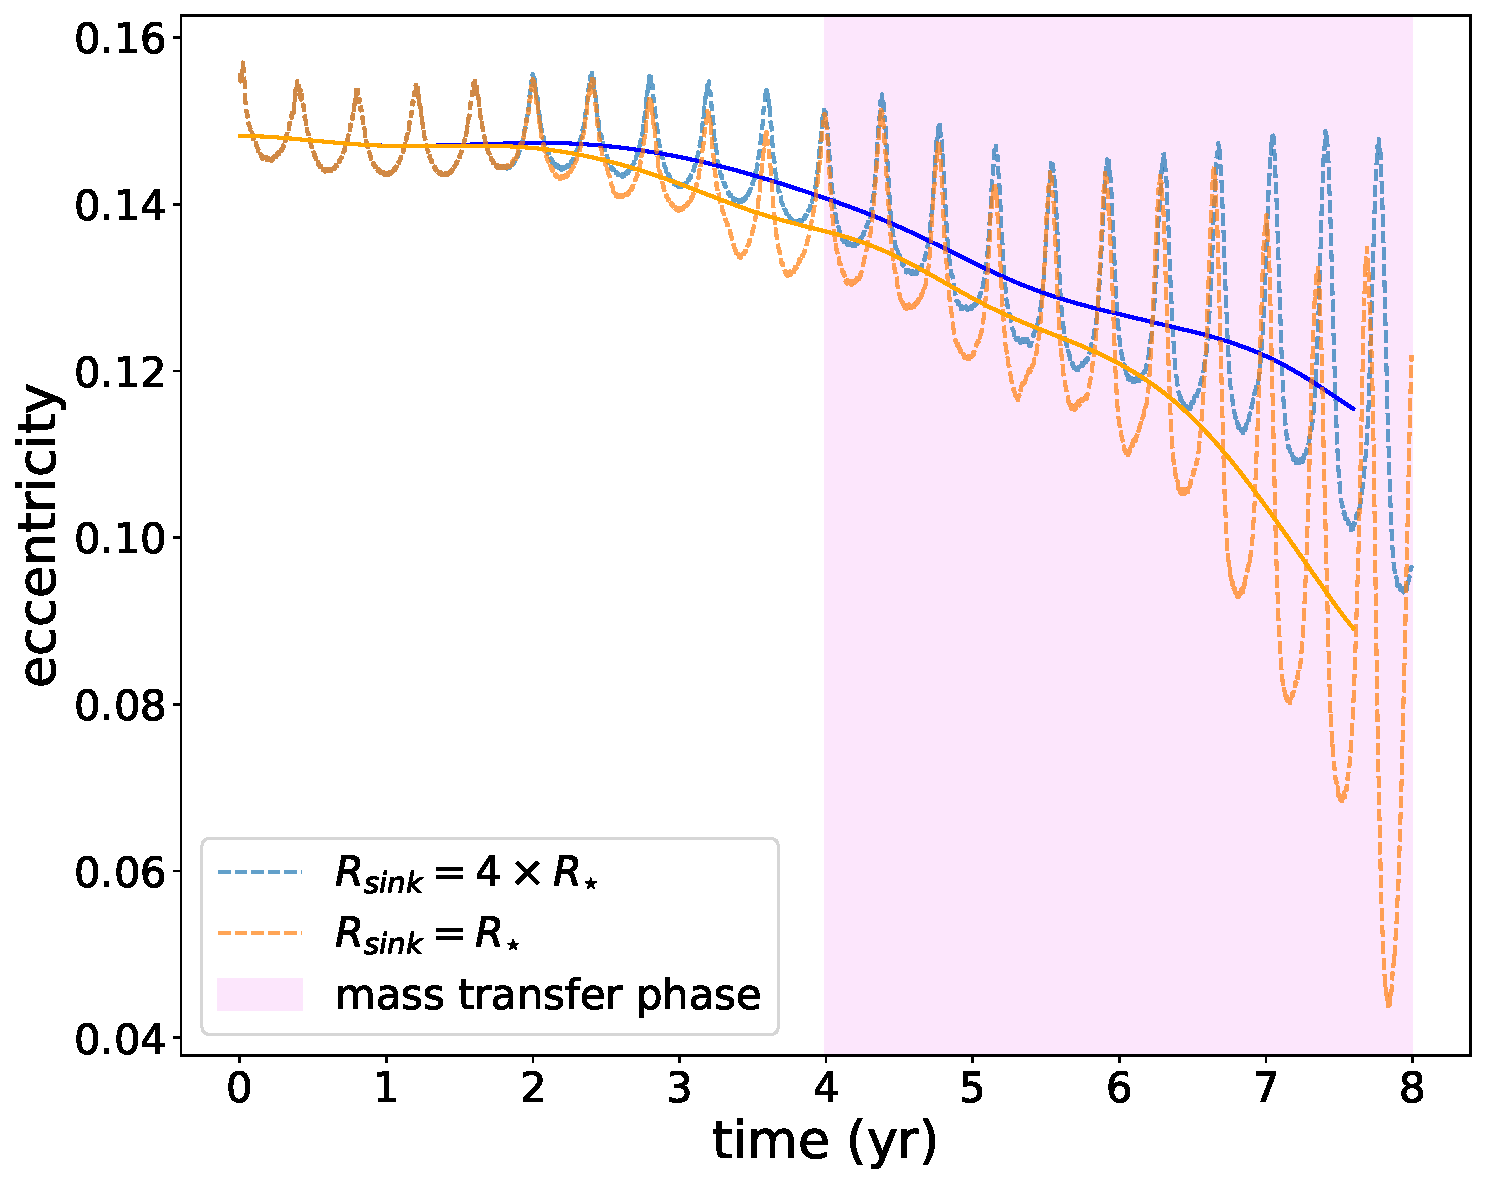
\includegraphics[width=0.76\textwidth]{Thesis/graphs/accretion_case/accretion_outer_ecc.pdf}
    \caption{Evolution of the eccentricity of the outer orbit for the minimum and maximum accretion case. The simulated data is shown in dashed lines. The continues lines are smooth representations of the simulated data in their respective colors. The last three orbits are not included in the smoothed version, because the lack of data above $8$ yr will erroneously flatten the slopes.}
    \label{fig:accretion_outer_ecc}
\end{figure}
\begin{comment}
\begin{figure}[H]
    \centering
    \begin{subfigure}{.5\textwidth}
    \centering
    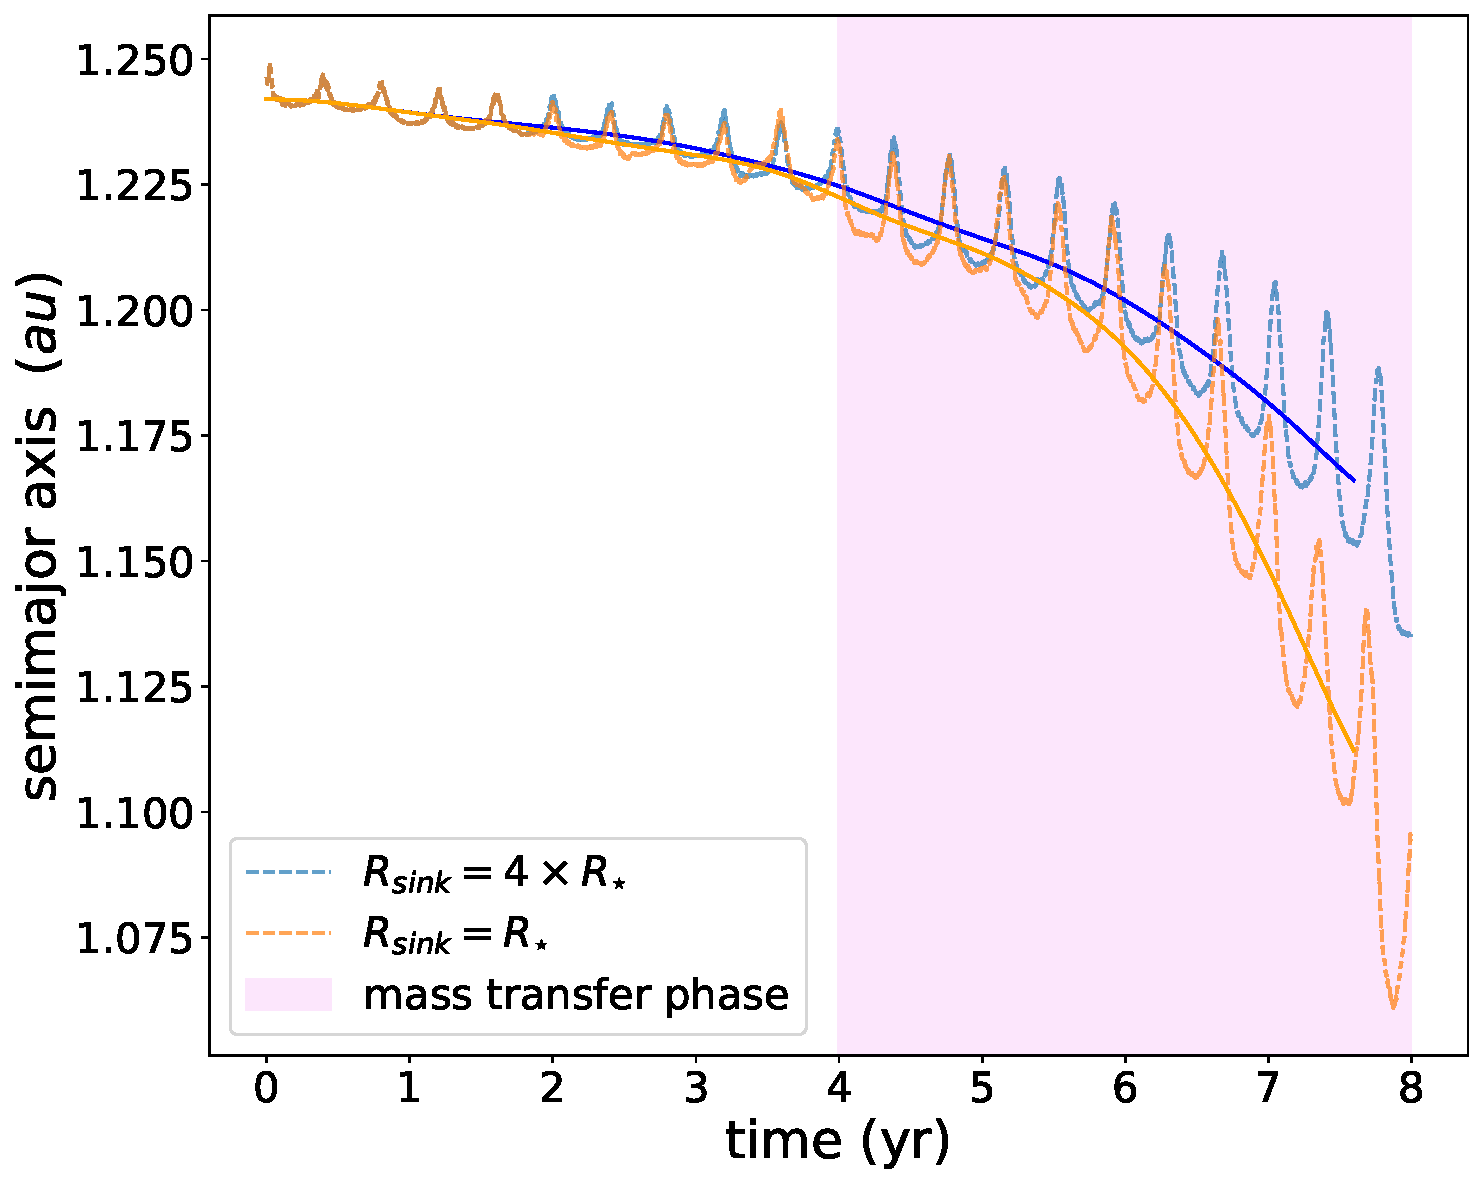
\includegraphics[width=0.9\textwidth]{Thesis/graphs/accretion_case/accretion_outer_semimajor_axis.pdf}
    \end{subfigure}%
    \begin{subfigure}{.5\textwidth}
    \centering
    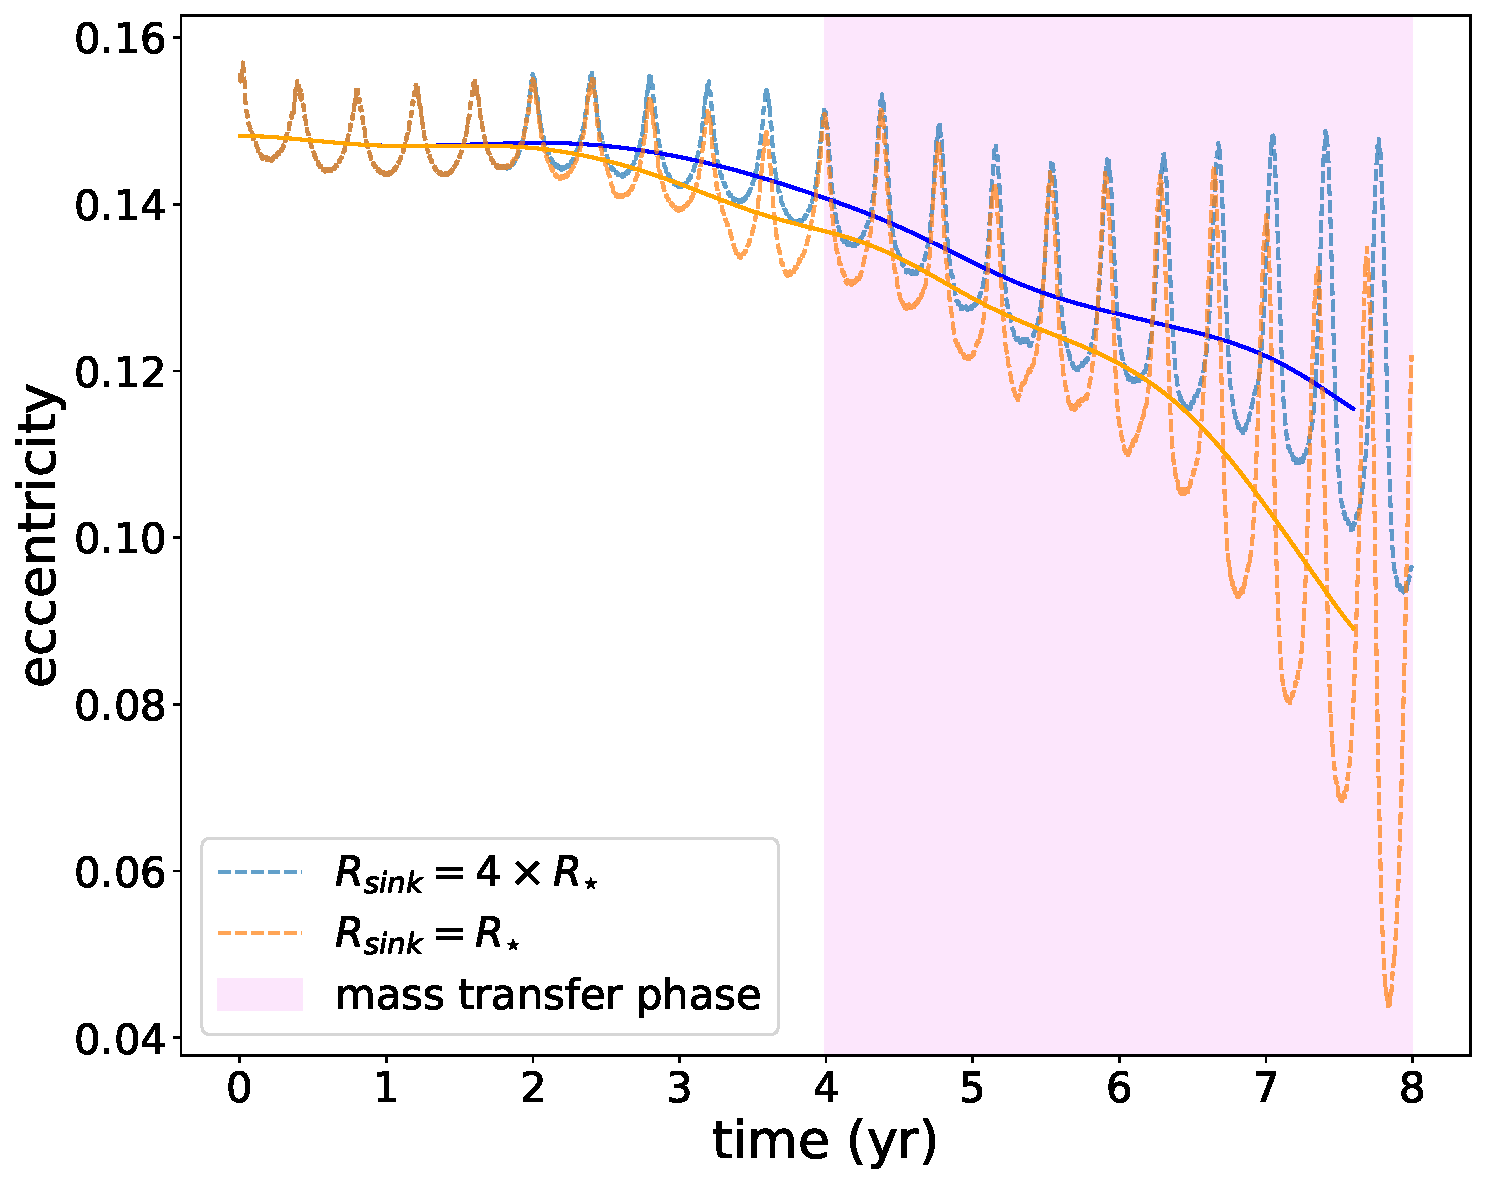
\includegraphics[width=0.9\textwidth]{Thesis/graphs/accretion_case/accretion_outer_ecc.pdf}
    \end{subfigure}
    \caption{ Evolution of the semi-major axis (left) and eccentricity (right) of the outer orbit}
    \label{fig:acc_outer_orbit}
\end{figure}
\end{comment}
\begin{figure}[!htb]
    \centering
    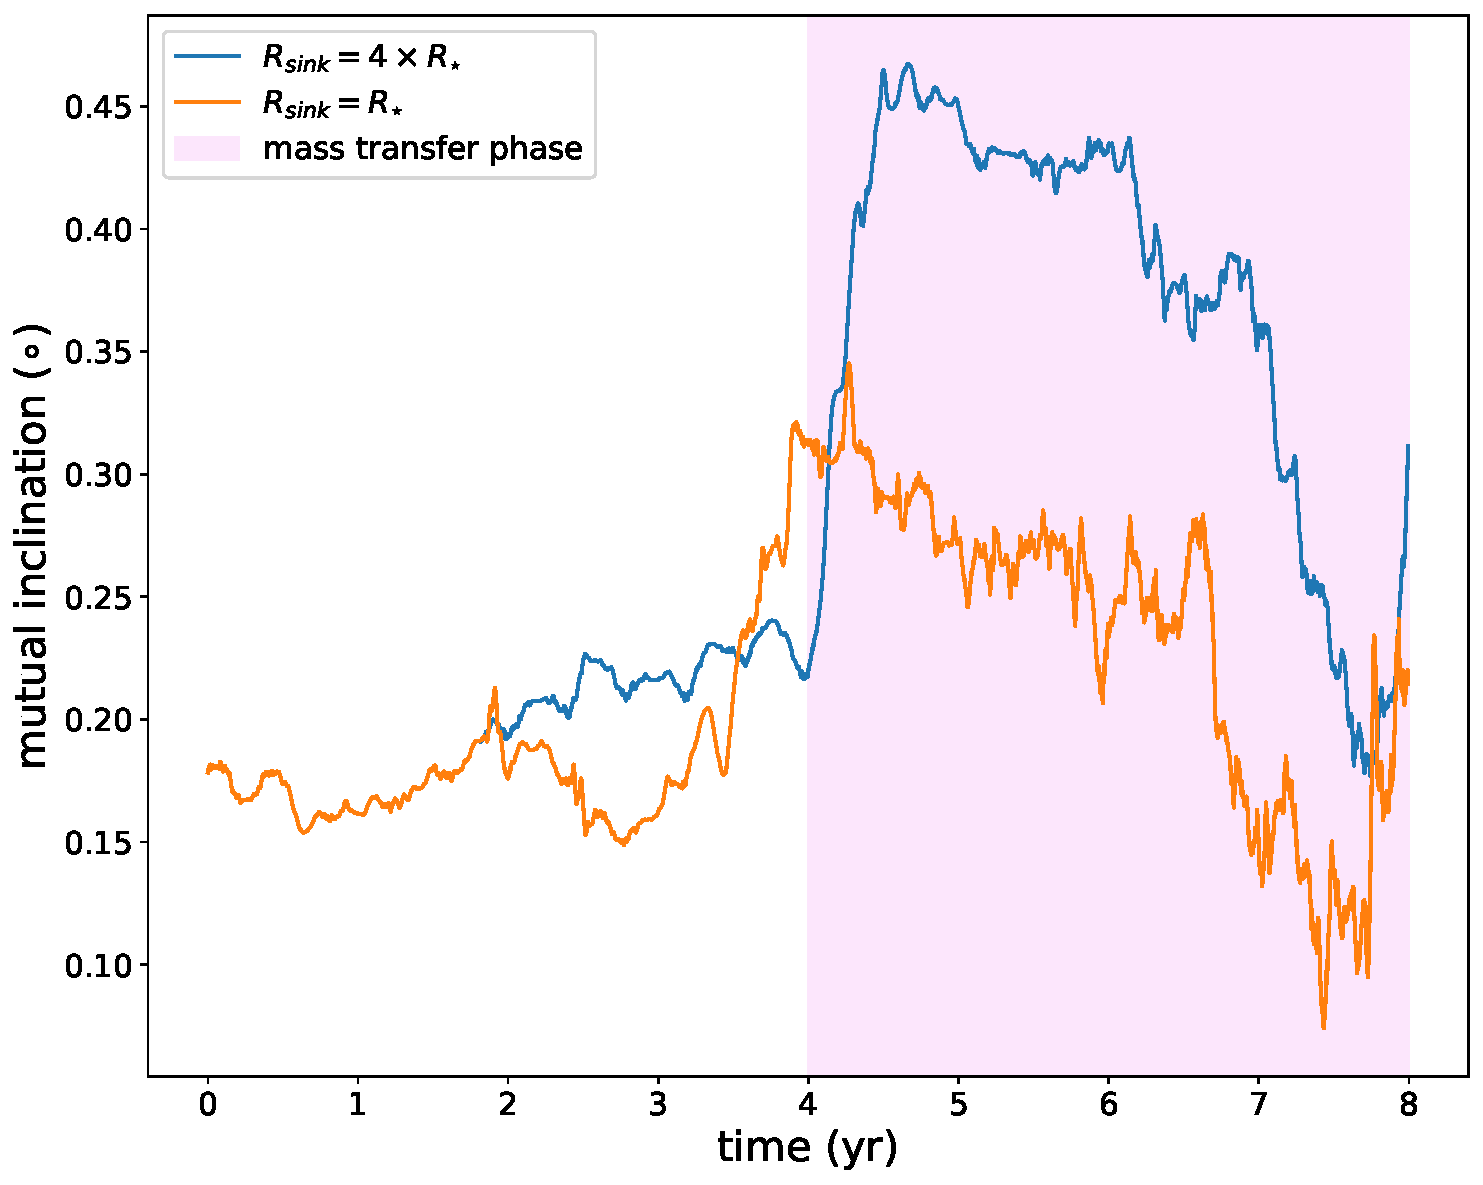
\includegraphics[width=0.76\textwidth]{Thesis/graphs/accretion_case/accretion_inc.pdf}
    \caption{Inclination of the outer orbit relative to the inner orbit.}
    \label{fig:accretion_inc}
\end{figure}
In \cref{fig:accretion_tertiary_mass}, I present the evolution of the tertiary's mass. The tertiary losses mass much faster in the minimum accretion case. The star's Roche lobe is proportional to its distance from the inner binary's center of mass; see \cref{eq:roche_lobe}, hence as the outer orbit decays faster, see \cref{fig:accretion_outer_semimajor_axis}, the tertiary's Roche lobe shrinks quicker. As a result, more and more gas overflows the Roche lobe and escapes towards the inner binary. To emphasize the difference in the mass evolution, I use central differentiation and provide mean mass loss rates for the simulated period, see \cref{fig:accretion_tertiary_mass}. The mass loss rates, should be taken with a grain of salt. Because the choice of $R_{\star} = 1.1 \times R_L$ significantly overestimates them, they should not be interpreted as average mass loss rates for RLOF, but they should be treated qualitatively. Despite that, it can not be ignored that the simulated values are in very good agreement with analytical ones calculated using \cref{eq:roche_lobe}.
\begin{figure}[H]
    \centering
    \begin{subfigure}{.5\textwidth}
    \centering
    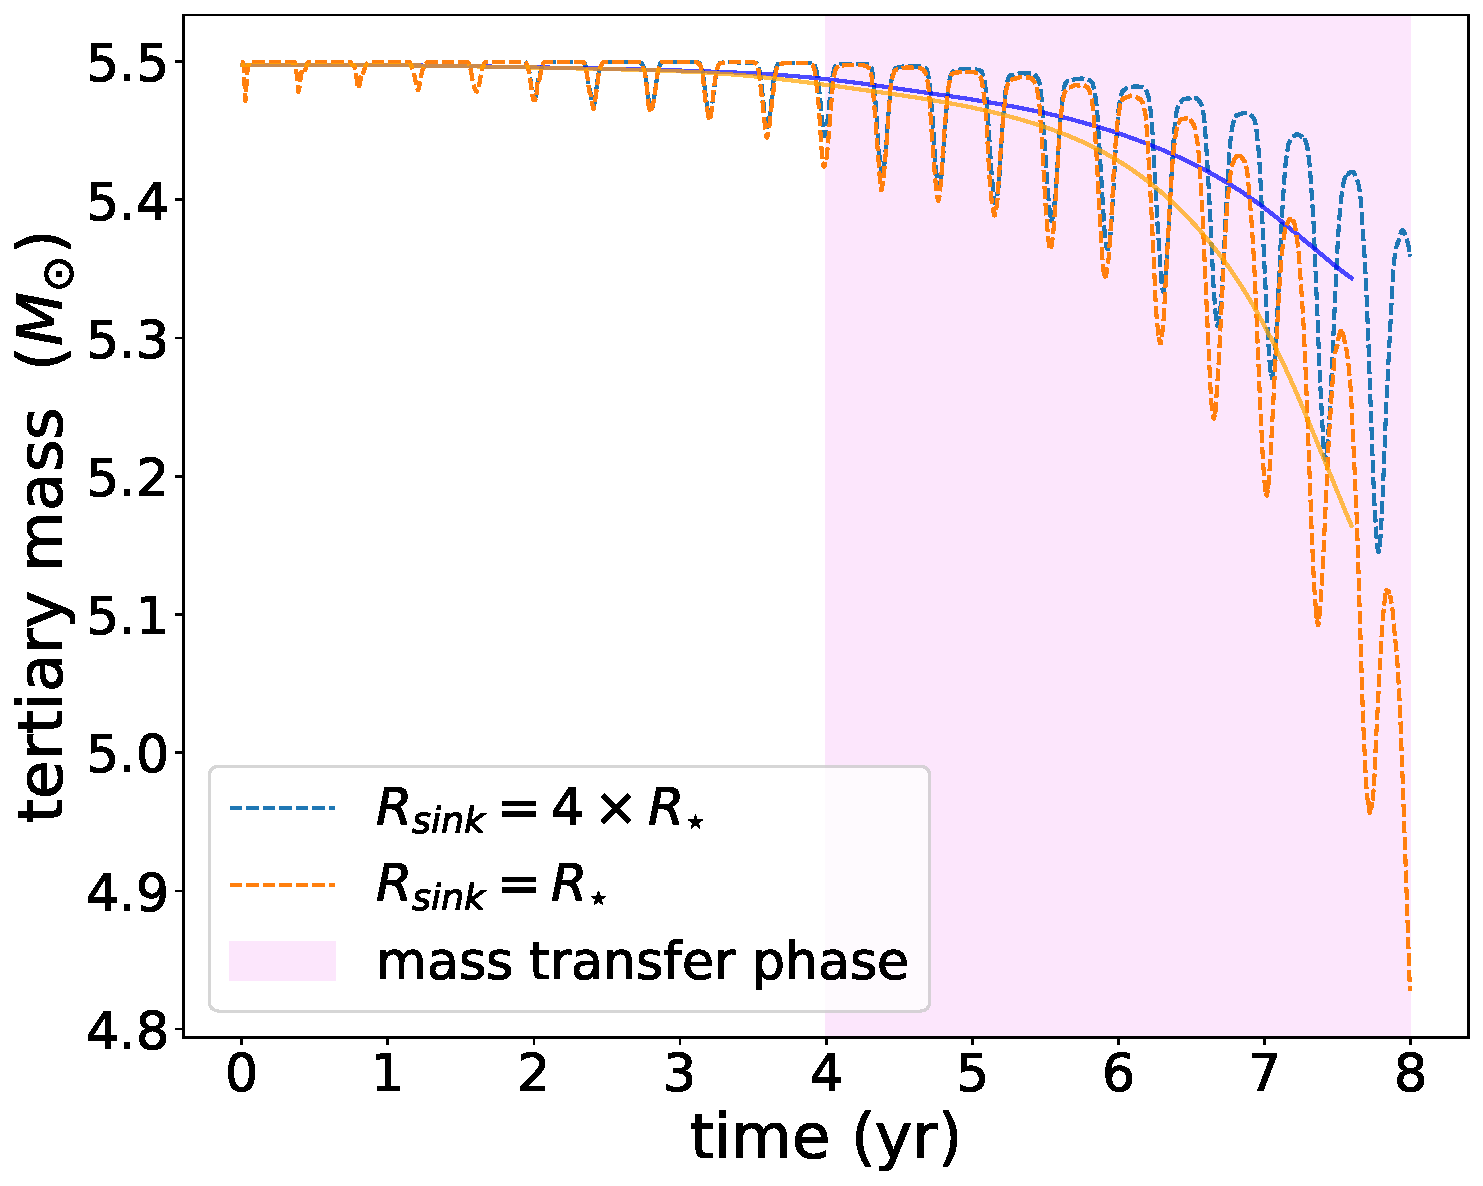
\includegraphics[width=0.9\textwidth]{Thesis/graphs/accretion_case/accretion_mass_loss.pdf}
    \end{subfigure}%
    \begin{subfigure}{.5\textwidth}
    \centering
    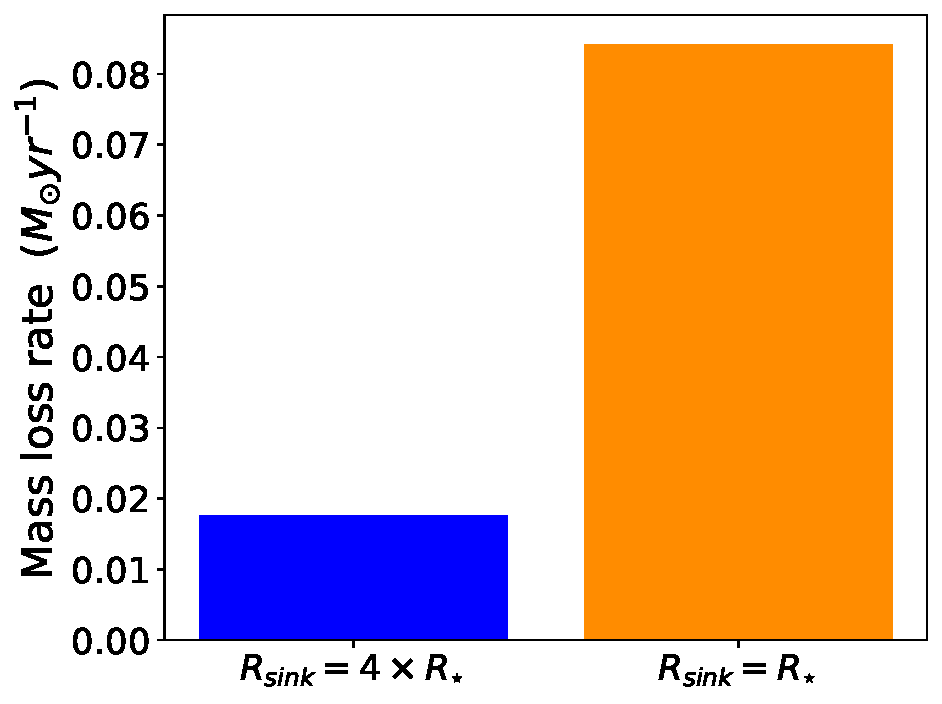
\includegraphics[width=0.9\textwidth]{Thesis/graphs/accretion_case/accretion_giant_mass_loss_rate.pdf}
    \end{subfigure}
    \caption{ The evolution of the tertiary's mass (left) for the minimum and maximum accretion case. The simulated data is shown in dashed lines. The continues lines are smooth representations of the simulated data in their respective colors. The last three orbits are not included in the smoothed version, because the lack of data above $8$ yr will erroneously flatten the slopes. The mean mass loss rates computed using central differentiation on the simulated data (right).}
    \label{fig:accretion_tertiary_mass}
\end{figure}


\subsection{Inner orbit}

In \cref{fig:accretion_inner_semimajor_axis} and \cref{fig:accretion_inner_ecc}, I present the evolution of the semi-major axis and eccentricity of the inner orbit, 
respectively. It is apparent that, the inner orbit widens in both the minimum and maximum accretion case. However, in the minimum accretion case, the orbit widens faster, see \cref{fig:accretion_inner_semimajor_axis}.
\begin{figure}[H]
    \centering
    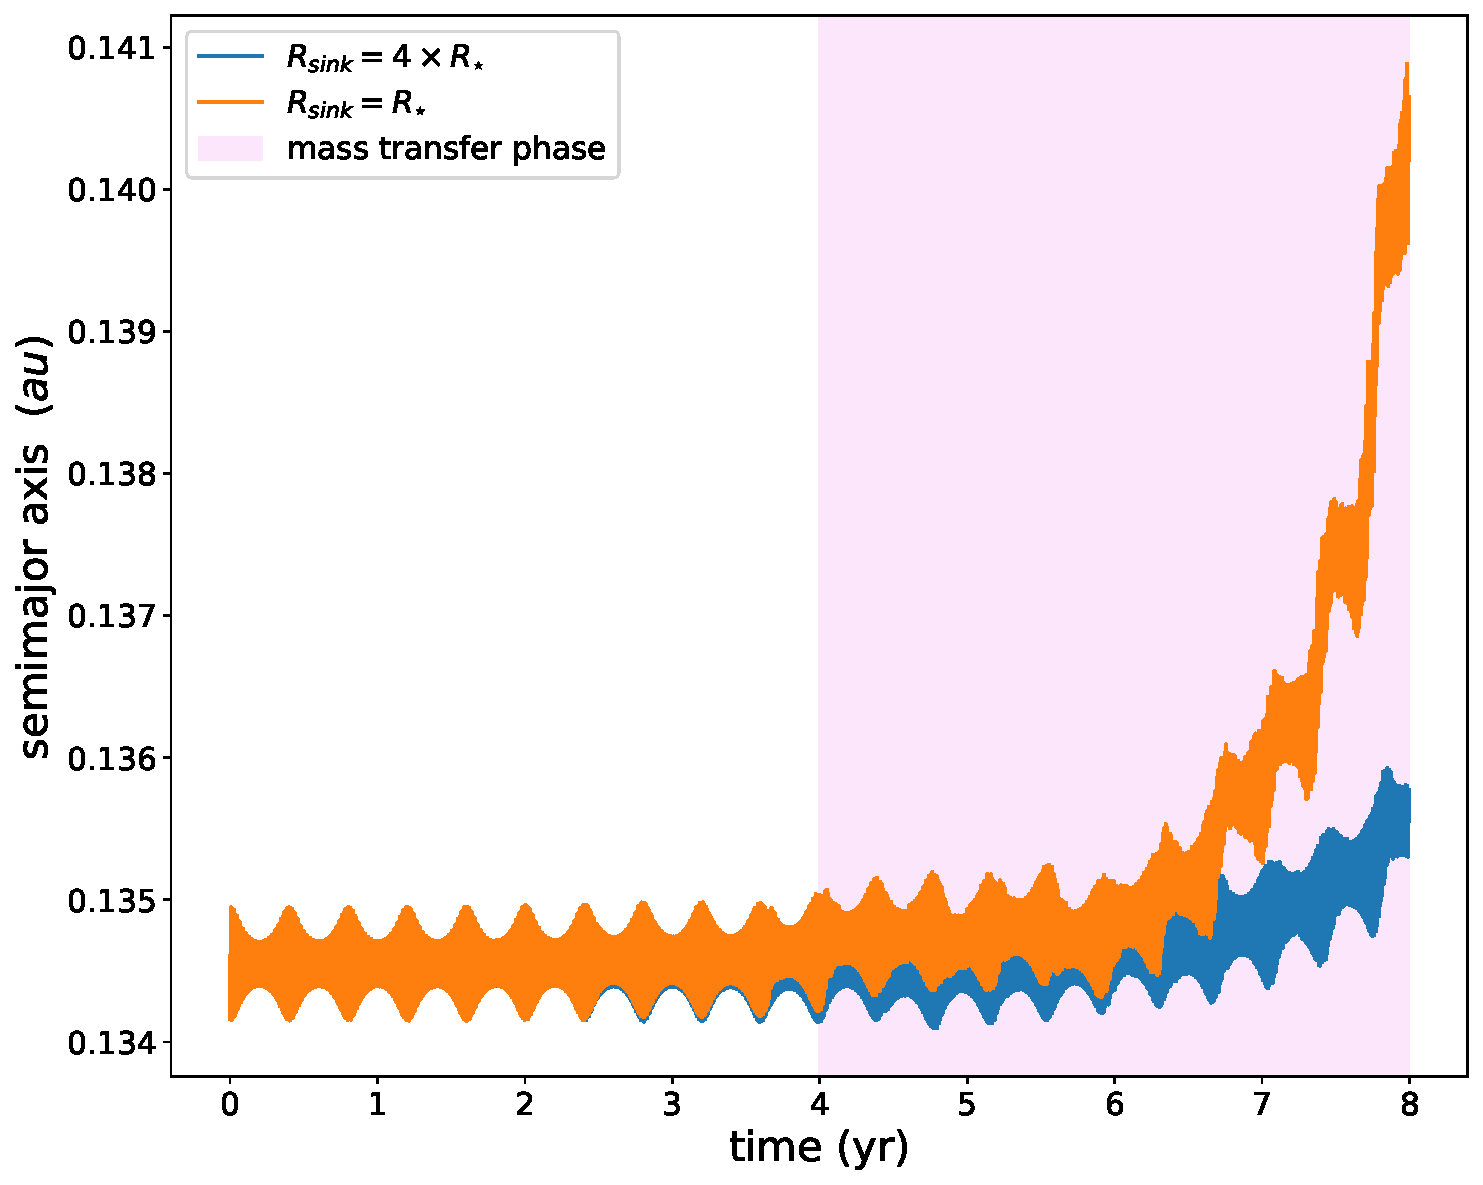
\includegraphics[width=0.9\textwidth]{Thesis/graphs/accretion_case/accretion_inner_semimajor_axis.pdf}
    \caption{Evolution of the semi-major axis of the inner orbit for the minimum and maximum accretion case.}
    \label{fig:accretion_inner_semimajor_axis}
\end{figure}
In the minimum accretion case, the tertiary's mass loss rate is much higher than the maximum accretion case, see \cref{fig:accretion_tertiary_mass} and the aforementioned trend is much more evident. Due to the underestimation of the effect of gas drag, the models are influenced by the gravitational interaction between the binary components and the incoming mass stream. The latter seems to result in a slingshot effect in favor of the the stars, see \cref{fig:retro} given that the orbital angular momentum of the inner and outer orbit are parallel. As more mass approaches the binary components, in the minimum accretion case, it can also approach them closer before it is being accreted, increasing the magnitude of the gravitational interactions. In conclusion, it is not possible to confidently draw conclusions about the impact of accretion on the inner orbit's semi-major axis given the current resolution. Finally, as expected, the effect of accretion on the eccentricity of the inner orbit is negligible. The orbit remains circular in both cases.
\begin{figure}[H]
    \centering
    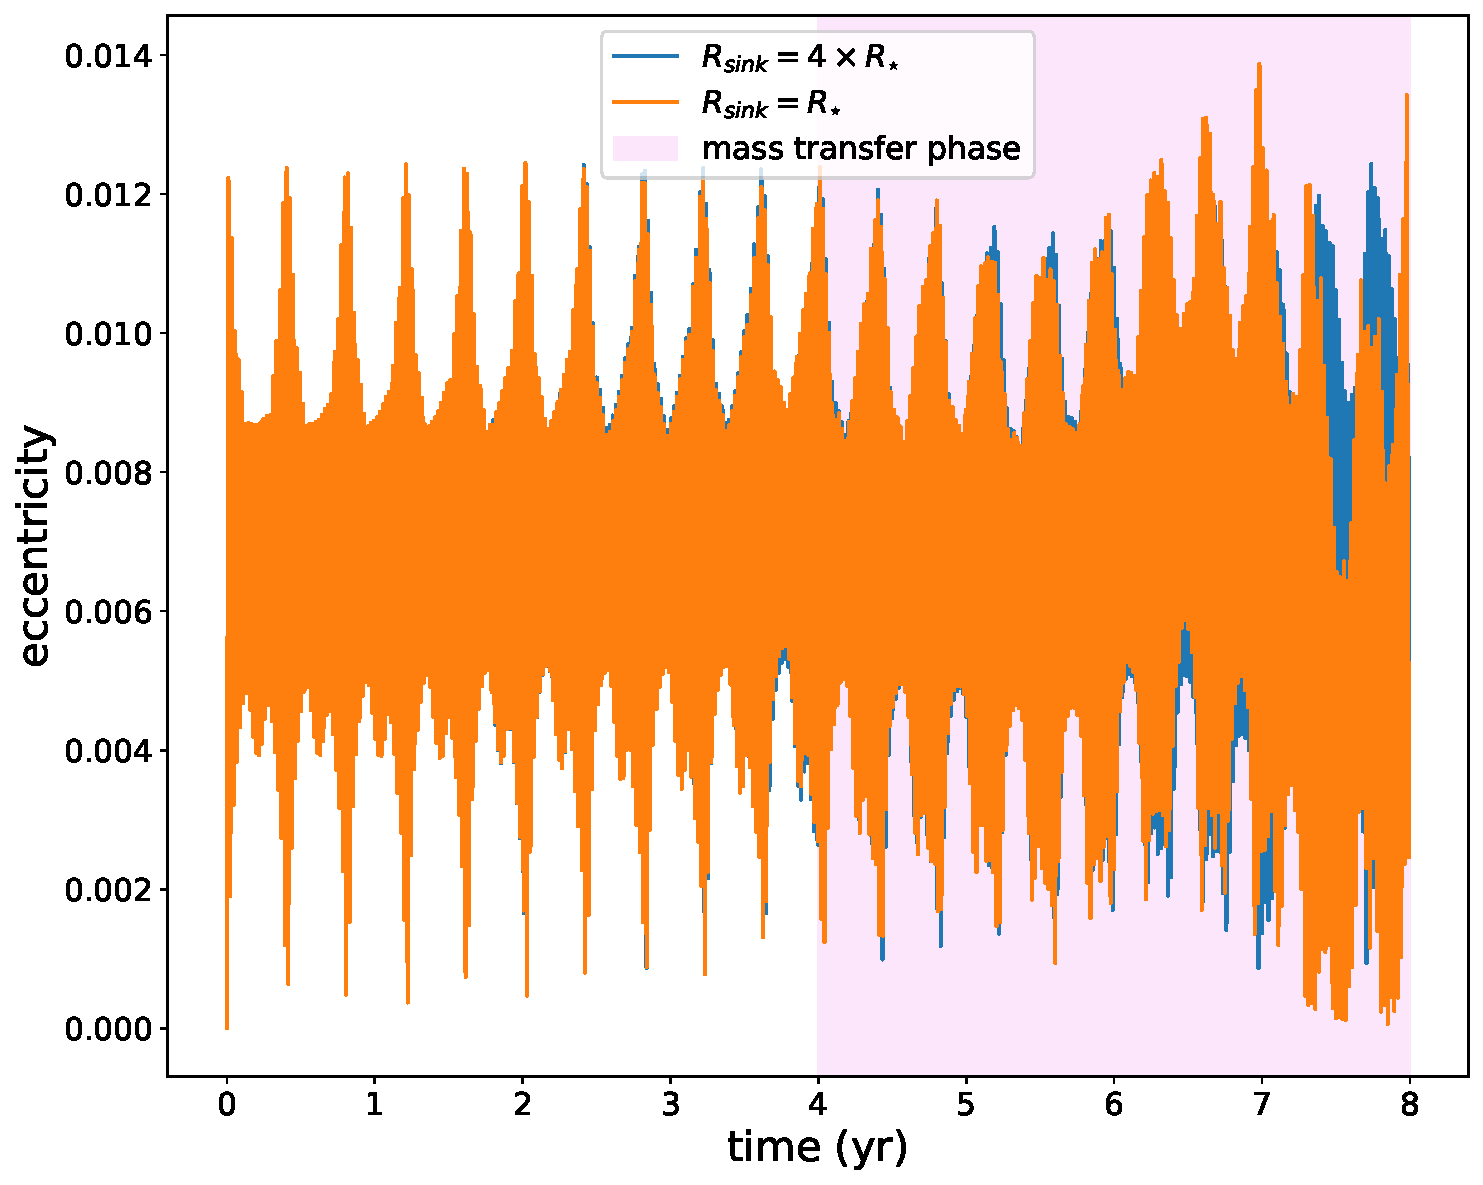
\includegraphics[width=0.9\textwidth]{Thesis/graphs/accretion_case/accretion_inner_ecc.pdf}
    \caption{Evolution of the eccentricity of the inner orbit for the minimum and maximum accretion case.}
    \label{fig:accretion_inner_ecc}
\end{figure}

\subsection{Analytical estimations}

During RLOF, matter from the outer donor star is either being accreted onto the inner binary stars, forms a disc around them, or is expelled from the triple system entirely. The orbits will change depending on what happens to the mass. This may be expressed in terms of the amount of angular momentum carried by the mass as it exits the donor star. On the one hand, the fraction of the accreted mass, $\beta$, and the amount of angular momentum that is carried away by the escaping mass are highly uncertain already in binary evolution studies. On the other hand, there are practically no theoretical predictions of the aforementioned quantities for mass transfer in hierarchical triples. More specifically, for the case of RLOF by an outer star towards the inner binary. 

In \cref{fig:accretion_eff_binary} I present an estimation of the accretion efficiency, $\beta$, for the maximum and minimum accretion case.
\begin{figure}[!htb]
    \centering
    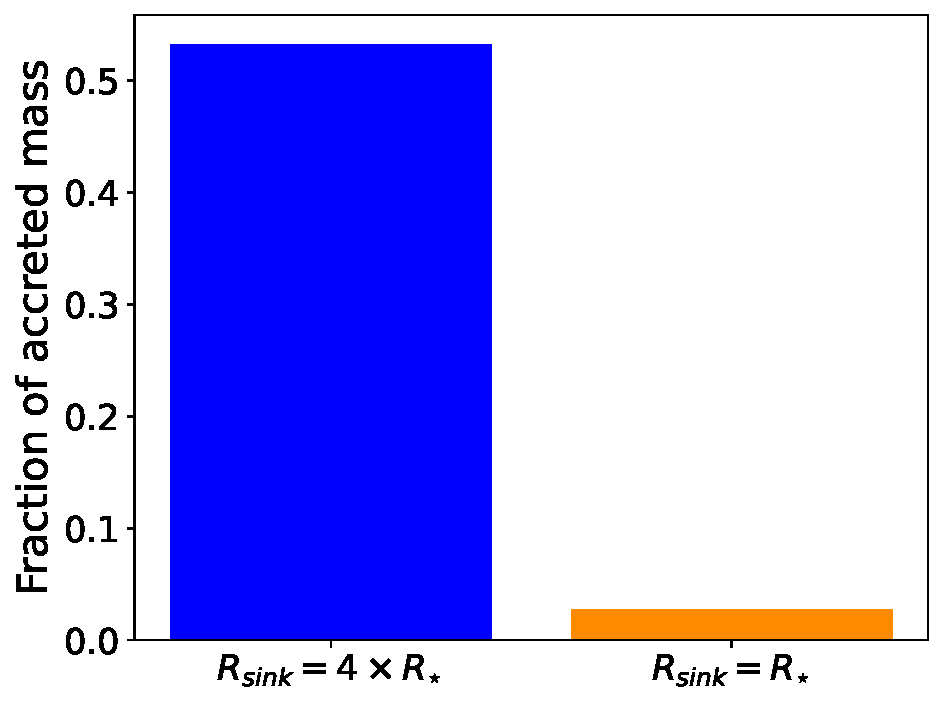
\includegraphics[width=0.9\textwidth]{Thesis/graphs/accretion_case/accretion_binary_acc_efficiency.pdf}
    \caption{Fraction of the accreted mass by the inner binary stars for the maximum and minim accretion cases.}
    \label{fig:accretion_eff_binary}
\end{figure}
In contrast to the concepts introduced in \cref{sub:orbit_evol_mass_loss}, $\beta$ corresponds to the fraction of mass being accreted by the inner binary. Nonetheless, $\beta = 0.53$ and $\beta = 0.03$ for the maximum and minimum accretion case, respectively. 

The absolute values presented, however, should be taken with a grain of salt. Higher resolution simulations are needed to examine the evolution of the inner semi-major axis, which may alter the details of the accretion process. Furthermore, the short period simulated here, can not capture additional parameters, which affect the fraction of accreted mass, $\beta$, such as the response of the accreting stars. The latter refers to the stars' envelope and rotational velocity response to the accreted mass. A more detailed discussion can be found in \cref{discussion}.

Despite the aforementioned uncertainties, the above outcome hints an intriguing possibility. The set up of the maximum accretion model intents to approach a conservative mass transfer scenario.
In \cite{zwart2019triple} study, the formation of a circumbinary disk leads to accretion efficiency up to $\beta \gtrsim 0.8$, despite the smaller accretion radii of the stars. In comparison, studies of conservative mass transfer in binaries report values of $\beta \geq 0.9$. As a result, it appears that, in the absence of a forming disk, the inner binary rotation makes accretion of incoming mass more difficult since part of it gets ejected via a slingshot effect. In conclusion, the accretion efficiency of the inner binary is most likely strongly related to whether or not a circumbinary disk forms. The absence of a forming disk suggests a highly non-conservative mass transfer.

On the one hand, the low resolution of the simulation and thus the underestimation of the gas drag does not allow for a direct comparison between analytical models and the evolution of the inner orbit's semi-major axis. On the other hand, the gas drag on the inner binary is mostly irrelevant for the evolution of the semi-major axis of the outer orbit, thus the amount of the lost angular momentum can be parameterized using analytical models.

In order to get an estimation about how much angular momentum is lost from the system, I compare the evolution of the semi-major axis of the outer orbit with the analytical model for non-conservative mass tranfer based on mass redistribution, see \cref{eq:semimajor_axis_no_cons}. The model assumes conservation of angular momentum despite the non-conservative case, similar to binaries as discussed by \cite{portegies1995formation}. Furthermore, it is assumed that the binary components are orbiting on the same plane, thus I compare the analytical model only with the models where $i_{mut}=0^{\circ}$, see \cref{tab:simulations_settings}.

Due to the fact that one component of the outer orbit is a binary system, the $M_a$ corresponds to its combined mass and $\eta$ is the specific angular momentum of the mass leaving the system as a proportion of the inner binary system's specific angular momentum. 
\begin{figure}[!htb]
    \centering
    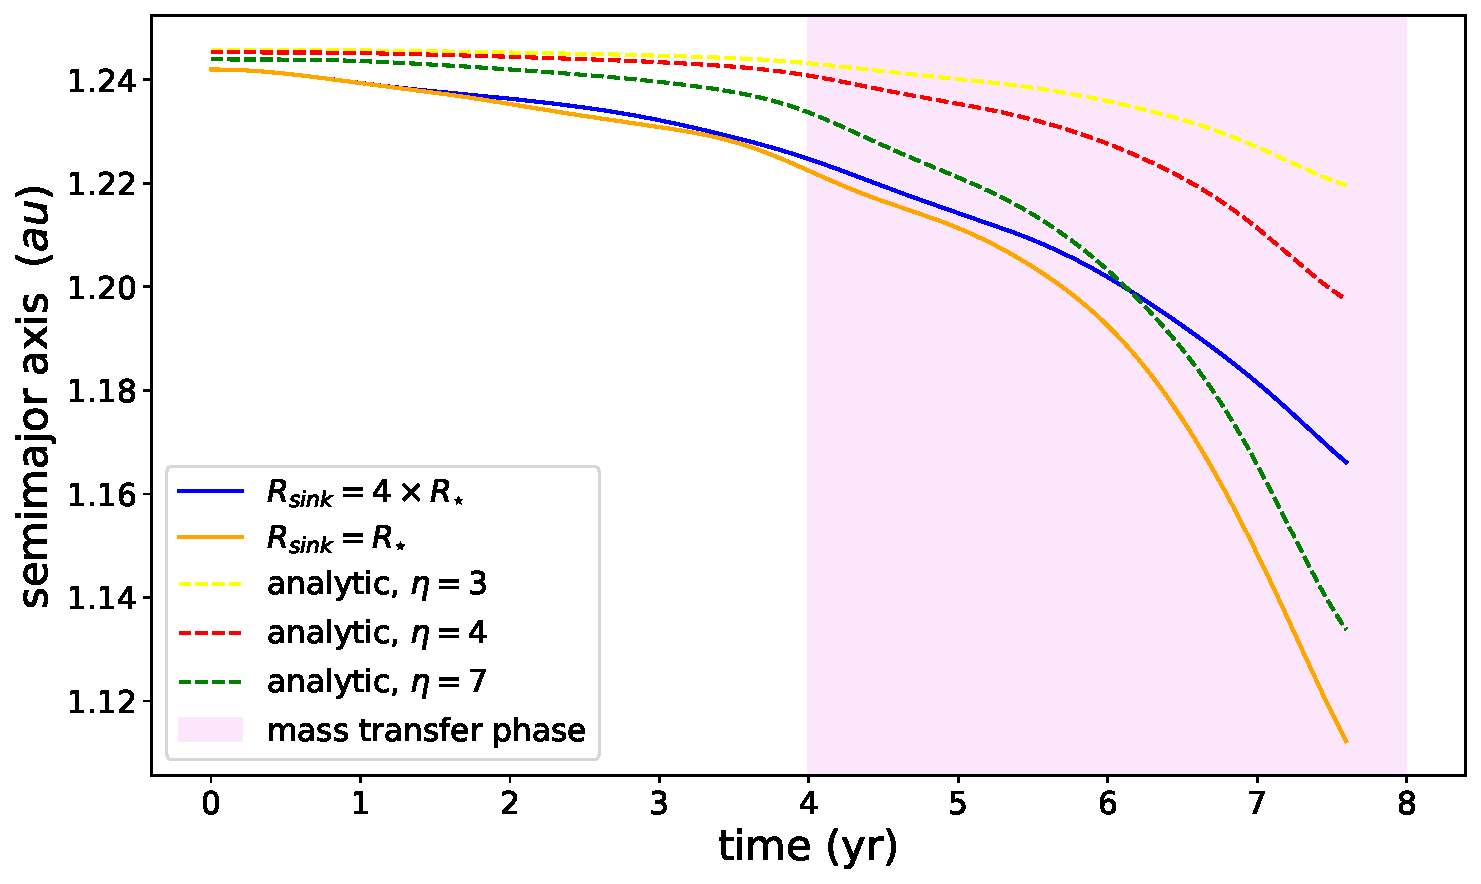
\includegraphics[width=0.85\textwidth]{Thesis/graphs/analytical_model.pdf}
    \caption{Evolution of the semi-major axis of the outer orbit for models number 1 and 4 listed in \cref{tab:simulations_settings}. The continues lines are representations of the simulated data, smoothed with a kernel with width $= 3 \times P_{out}$. The dashed lines correspond to analytical models in yellow, red, green and black, respectively.  The last three orbits are not included in the smoothed version, because the lack of data above $8$ yr will erroneously flatten the slopes.}
    \label{fig:comparison_analytical_model_max}
\end{figure}
In \cref{fig:comparison_analytical_model_max}, I present smoothed versions of the simulated data in blue and orange for the maximum and minimum accretion case, respectively. I also overplot four models, based on the maximum accretion case using \cref{eq:semi-major_axis}, for $\eta = 3,4,7,10$. Higher value of $\eta$ indicate that a higher amount of angular momentum is carried away by the ejected mass. During the mass transfer phase a model with $\eta \approx 4$ matches the slope of the orbital evolution for the maximum accretion case, while a model with $\eta \approx 7$ matches the minimum accretion case's orbital evolution slope. The graph indicates that in the maximum accretion case, given the same amount of ejected mass, the latter should carry significantly more angular momentum in order to match the minimum accretion case ($\eta = 7$). Hence, it is evident that the efficiency of the accretion process is vital for the timescale of the outer orbit's decay and consequently for the triple system's evolution.






\section{Impact of initial mutual inclination}\label{sec:inclination}


In this section, I investigate the importance of the initial mutual inclination on the evolution of the system. I present a comparison between simulations  1, 2 \& 3 listed in \cref{tab:simulations_settings}, which correspond to different initial inclination of the outer orbit relative to the inner orbit


\subsection{Outer orbit}

In \cref{fig:incliantion_tertiary_mass}, I present the evolution of the tertiary's mass for different initial mutual inclination. First, I would like to point out that the case of $i_{mut} = 69^{\circ}$ is not directly comparable to the other two cases. In order to place the tertiary initially at a higher inclination, the positions of all particles in the 3D model are corrected for the appropriate angle. Then the center of mass of the tertiary corresponds to the center of mass of all these particles. In this case, numerical rounding resulted into a shorter initial separation between the giant and the center of mass of the inner binary, see \cref{fig:inclination_outer_semimajor_axis}. More specifically, the tertiary was placed $\approx 0.01$ au ($\approx 2.15 R_{\odot}$) closer. This may seem as a small difference, but it has a significant impact on the mass loss rate. The smaller initial separation corresponds to higher fractional radius excess of the tertiary and considering \cref{eq:mass_loss_rate_anal}, the mass loss rate is highly overestimated in comparison with the other two models, see also \cref{fig:incliantion_tertiary_mass}.  As a result, the rate of decay of the outer orbit for the $i_{mut} = 69^{\circ}$ case is also overestimated compared to the other two models.
\begin{figure}[!htb]
    \centering
    \begin{subfigure}{.5\textwidth}
    \centering
    \includegraphics[width=0.9\textwidth]{Thesis/graphs/inclination_case/inclination_mass_loss.pdf}
    \end{subfigure}%
    \begin{subfigure}{.5\textwidth}
    \centering
    \includegraphics[width=0.9\textwidth]{Thesis/graphs/inclination_case/incliantion_giant_mass_loss_rate.pdf}
    \end{subfigure}
    \caption{ The evolution of the tertiary's mass (left) for of the outer orbit for different initial inclination of the outer orbit relative to the inner orbit. The simulated data is shown in dashed lines. The continues lines are smooth representations of the simulated data in their respective colors. The last three orbits are not included in the smoothed version, because the lack of data above $8$ yr will erroneously flatten the slopes. The mean mass loss rates computed using central differentiation on the simulated data (right).}
    \label{fig:incliantion_tertiary_mass}
\end{figure}

Keeping in mind that the mass loss rate for the case of $i_{mut} = 69^{\circ}$ is overestimated, I speculate that there is a trend: lower initial mutual inclination results to higher mass loss rate for the tertiary. This is not a surprise, as each of the inner binary stars can approach the giant closer for orbits that are nearly on the same plane. Additionally, the mass loss rate derived using central differentiation on the simulated data are in good agreement with the analytical ones calculated using \cref{eq:mass_loss_rate_anal}.
\begin{figure}[H]
    \centering
    \includegraphics[width=0.85\textwidth]{Thesis/graphs/inclination_case/inclination_outer_semimajor_axis.pdf}
    \caption{Evolution of the semi-major axis of the outer orbit for different initial inclination of the outer orbit relative to the inner orbit. The simulated data is shown in dashed lines. The continues lines are smooth representations of the simulated data in their respective colors. The last three orbits are not included in the smoothed version, because the lack of data above $8$ yr will erroneously flatten the slopes.}
    \label{fig:inclination_outer_semimajor_axis}
\end{figure}
In \cref{fig:inclination_outer_semimajor_axis}, I display the evolution of the semi-major axis for different initial mutual inclinations. Considering only the $i_{mut} = 0^{\circ} \; \&  \; 20^{\circ}$ cases, the outer orbit decays faster for lower initial mutual inclination, because more mass is transferred towards the inner binary carrying away orbital angular momentum. 

In \cref{fig:inclination_outer_ecc},  the evolution of the eccentricity for different initial mutual inclinations is illustrated. Furthermore, in \cref{fig:mutual_inclination}, I present the evolution of the mutual inclination between the inner and the outer orbit for initial $i_{mut} = 20^{\circ}, 69^{\circ}$. The $i_{mut} = 0^{\circ}$ case is already displayed in \cref{fig:accretion_inc}.  Tidal interactions, as predicted, tend to circularize the outer orbit and also bring it towards coplanarity with the inner orbit.
\begin{figure}[H]
    \centering
    \includegraphics[width=0.9\textwidth]{Thesis/graphs/inclination_case/inclination_outer_ecc.pdf}
    \caption{Evolution of the eccentricity of the outer orbit for different initial inclination of the outer orbit relative to the inner orbit. The simulated data is shown in dashed lines. The continues lines are smooth representations of the simulated data in their respective colors. The last three orbits are not included in the smoothed version, because the lack of data above $8$ yr will erroneously flatten the slopes.}
    \label{fig:inclination_outer_ecc}
\end{figure}
As the giant, approaches the inner binary, the outer orbit tends to be circular, see \cref{fig:inclination_outer_ecc}. The interesting point though comes from a comparison between $i_{mut} = 20^{\circ} \& 69^{\circ}$. Despite the fact that for $i_{mut} = 69^{\circ}$ the giant has a higher mass loss rate and is closer $\sim 0.05$ au to the center of mass of the inner binary, see \cref{fig:inclination_outer_semimajor_axis}, the orbit circularizes faster for $i_{mut} = 20^{\circ}$. The individual inner binary stars can approach the giant closer for orbits that are nearly on the same plane, hence tidal interactions are expected to be stronger. The decay of the mutual inclination seems to be equivalent in both cases. The conclusion is that the effect of the hydrodynamics on the decay of the eccentricity and mutual inclination of the outer orbit is probably negligible. Both parameters are mostly affected by tidal interactions between the two orbits.
\begin{figure}[H]
    \centering
    \begin{subfigure}{.5\textwidth}
    \centering
    \includegraphics[width=0.9\textwidth]{Thesis/graphs/inclination_case/inc_20.pdf}
    \end{subfigure}%
    \begin{subfigure}{.5\textwidth}
    \centering
    \includegraphics[width=0.9\textwidth]{Thesis/graphs/inclination_case/inc_69.pdf}
    \end{subfigure}
    \caption{ The evolution of the inclination of the outer orbit relative to the inner orbit for initial value: $i_{mut}=20^{\circ}$ (left) and $i_{mut}=69^{\circ}$ (right).}
    \label{fig:mutual_inclination}
\end{figure}

\subsection{Inner orbit}

In \cref{fig:inclination_inner_semimajor_axis} and \cref{fig:inclination_inner_ecc}, I present the evolution of the semi-major axis and eccentricity of the inner orbit for different initial mutual inclinations, respectively. The observed behavior for low inclinations, such as $i_{mut}=0^{\circ}, 20^{\circ}$, has already been described in \cref{sec:accretion}, but the case of $i_{mut}=69^{\circ}$ yields some intriguing results.

Despite underestimating the gas drag, it is evident that I can still extract some valuable insights regarding the evolution of the inner orbit. The inner orbit shrinks with the greatest initial mutual inclination. The reason for this behavior is that the mass stream can successfully cross the inner orbit at high angles, draining orbital angular momentum from the latter. Additionally, because gas drag always tends to shrink the orbit, the observed behavior is qualitatively accurate. The only difference is that including gas drag, the rate of the orbit's decay will be higher or in simple words the observed slope will be steeper. 
\begin{figure}[H]
    \centering
    \includegraphics[width=0.9\textwidth]{Thesis/graphs/inclination_case/inclination_inner_semimajor_axis.pdf}
    \caption{Evolution of the semi-major axis of the inner orbit for different initial mutual inclination.}
    \label{fig:inclination_inner_semimajor_axis}
\end{figure}
The $i_{mut}=69^{\circ}$ value was selected intentionally, to test the accuracy of the coupled solver. It is clear, that the latter can resolve Lidov-Kozai cycles. The $i_{mut}=69^{\circ}$ is well inside in the regime where the Lidov-Kozai cycles are expected to occur, see \cref{sub:lidov_kozai}. The eccentricity and mutual inclination are expected to vary periodically. As expected, as the eccentricity increases and the mutual inclination decreases, see \cref{fig:mutual_inclination} and \cref{fig:inclination_inner_semimajor_axis}.
\begin{figure}[!htb]
    \centering
    \includegraphics[width=0.9\textwidth]{Thesis/graphs/inclination_case/inclination_inner_ecc.pdf}
    \caption{Evolution of the semi-major axis of the inner orbit for different initial mutual inclination.}
    \label{fig:inclination_inner_ecc}
\end{figure}



\begin{comment}
    On one hand, on the current resolution the gas drag is considerably underestimated. On the other hand, the gravitational interactions of the mass stream with the inner binary seems to act like a scattering process, but in favor of the stars. 



Finally, it is important to mention that after analyzing my data, it became clear that the resolution of my simulations was insufficient to accurately capture the influence of the gas drag on the inner orbit. As a result, the gas drag is underestimated, while the models capture the gravitational interactions between the inner binary, the core of the tertiary, and its gaseous envelope.  A detailed discussion over the low resolution and the gas drag is provided in \cref{discussion}.
\end{comment}




.

\chapter{Discussion \& Conclusions}\label{discussion}










In this case, the angular momentum vectors of the inner binary and the inflowing gas are (almost) aligned, hence less angular momentum is required to accelerate the gas to the escape velocity. Furthermore, on the current resolution the gas drag is considerably underestimated.

Indeed, when the angular momentum vectors of the inner binary and the inflowing gas are (almost) aligned, less angular momentum needs to be transferred to speed up the gas to the escape velocity.







\section{Discussion}

In this section, I describe some crucial features of the modeling method that will assist the reader in interpreting the graphs, presented in the next sections. 

\appendix

\chapter*{Appendix}

The are a few ways to numerically approximate derivatives of functions and central differentiation is the most accurate one. My goal is to estimate the slope of a curve $f$ at a certain location $x = a$ using $f(a)$ and the value of $f$ at a neighboring point $x = a + h$. If $h$ is small enough, the shorter broken line in Figure 11 can be regarded of as an acceptable approximation to the requisite slope (indicated by the longer broken line).

\newpage

\bibliographystyle{plainnat}
\bibliography{refs}

%## IMPORTANT#############################################
\acuseall
%## IMPORTANT#############################################
\end{document}